% Options for packages loaded elsewhere
\PassOptionsToPackage{unicode}{hyperref}
\PassOptionsToPackage{hyphens}{url}
\PassOptionsToPackage{dvipsnames,svgnames,x11names}{xcolor}
%
\documentclass[
  letterpaper,
  DIV=11,
  numbers=noendperiod]{scrreprt}

\usepackage{amsmath,amssymb}
\usepackage{lmodern}
\usepackage{iftex}
\ifPDFTeX
  \usepackage[T1]{fontenc}
  \usepackage[utf8]{inputenc}
  \usepackage{textcomp} % provide euro and other symbols
\else % if luatex or xetex
  \usepackage{unicode-math}
  \defaultfontfeatures{Scale=MatchLowercase}
  \defaultfontfeatures[\rmfamily]{Ligatures=TeX,Scale=1}
\fi
% Use upquote if available, for straight quotes in verbatim environments
\IfFileExists{upquote.sty}{\usepackage{upquote}}{}
\IfFileExists{microtype.sty}{% use microtype if available
  \usepackage[]{microtype}
  \UseMicrotypeSet[protrusion]{basicmath} % disable protrusion for tt fonts
}{}
\makeatletter
\@ifundefined{KOMAClassName}{% if non-KOMA class
  \IfFileExists{parskip.sty}{%
    \usepackage{parskip}
  }{% else
    \setlength{\parindent}{0pt}
    \setlength{\parskip}{6pt plus 2pt minus 1pt}}
}{% if KOMA class
  \KOMAoptions{parskip=half}}
\makeatother
\usepackage{xcolor}
\setlength{\emergencystretch}{3em} % prevent overfull lines
\setcounter{secnumdepth}{5}
% Make \paragraph and \subparagraph free-standing
\ifx\paragraph\undefined\else
  \let\oldparagraph\paragraph
  \renewcommand{\paragraph}[1]{\oldparagraph{#1}\mbox{}}
\fi
\ifx\subparagraph\undefined\else
  \let\oldsubparagraph\subparagraph
  \renewcommand{\subparagraph}[1]{\oldsubparagraph{#1}\mbox{}}
\fi

\usepackage{color}
\usepackage{fancyvrb}
\newcommand{\VerbBar}{|}
\newcommand{\VERB}{\Verb[commandchars=\\\{\}]}
\DefineVerbatimEnvironment{Highlighting}{Verbatim}{commandchars=\\\{\}}
% Add ',fontsize=\small' for more characters per line
\usepackage{framed}
\definecolor{shadecolor}{RGB}{241,243,245}
\newenvironment{Shaded}{\begin{snugshade}}{\end{snugshade}}
\newcommand{\AlertTok}[1]{\textcolor[rgb]{0.68,0.00,0.00}{#1}}
\newcommand{\AnnotationTok}[1]{\textcolor[rgb]{0.37,0.37,0.37}{#1}}
\newcommand{\AttributeTok}[1]{\textcolor[rgb]{0.40,0.45,0.13}{#1}}
\newcommand{\BaseNTok}[1]{\textcolor[rgb]{0.68,0.00,0.00}{#1}}
\newcommand{\BuiltInTok}[1]{\textcolor[rgb]{0.00,0.23,0.31}{#1}}
\newcommand{\CharTok}[1]{\textcolor[rgb]{0.13,0.47,0.30}{#1}}
\newcommand{\CommentTok}[1]{\textcolor[rgb]{0.37,0.37,0.37}{#1}}
\newcommand{\CommentVarTok}[1]{\textcolor[rgb]{0.37,0.37,0.37}{\textit{#1}}}
\newcommand{\ConstantTok}[1]{\textcolor[rgb]{0.56,0.35,0.01}{#1}}
\newcommand{\ControlFlowTok}[1]{\textcolor[rgb]{0.00,0.23,0.31}{#1}}
\newcommand{\DataTypeTok}[1]{\textcolor[rgb]{0.68,0.00,0.00}{#1}}
\newcommand{\DecValTok}[1]{\textcolor[rgb]{0.68,0.00,0.00}{#1}}
\newcommand{\DocumentationTok}[1]{\textcolor[rgb]{0.37,0.37,0.37}{\textit{#1}}}
\newcommand{\ErrorTok}[1]{\textcolor[rgb]{0.68,0.00,0.00}{#1}}
\newcommand{\ExtensionTok}[1]{\textcolor[rgb]{0.00,0.23,0.31}{#1}}
\newcommand{\FloatTok}[1]{\textcolor[rgb]{0.68,0.00,0.00}{#1}}
\newcommand{\FunctionTok}[1]{\textcolor[rgb]{0.28,0.35,0.67}{#1}}
\newcommand{\ImportTok}[1]{\textcolor[rgb]{0.00,0.46,0.62}{#1}}
\newcommand{\InformationTok}[1]{\textcolor[rgb]{0.37,0.37,0.37}{#1}}
\newcommand{\KeywordTok}[1]{\textcolor[rgb]{0.00,0.23,0.31}{#1}}
\newcommand{\NormalTok}[1]{\textcolor[rgb]{0.00,0.23,0.31}{#1}}
\newcommand{\OperatorTok}[1]{\textcolor[rgb]{0.37,0.37,0.37}{#1}}
\newcommand{\OtherTok}[1]{\textcolor[rgb]{0.00,0.23,0.31}{#1}}
\newcommand{\PreprocessorTok}[1]{\textcolor[rgb]{0.68,0.00,0.00}{#1}}
\newcommand{\RegionMarkerTok}[1]{\textcolor[rgb]{0.00,0.23,0.31}{#1}}
\newcommand{\SpecialCharTok}[1]{\textcolor[rgb]{0.37,0.37,0.37}{#1}}
\newcommand{\SpecialStringTok}[1]{\textcolor[rgb]{0.13,0.47,0.30}{#1}}
\newcommand{\StringTok}[1]{\textcolor[rgb]{0.13,0.47,0.30}{#1}}
\newcommand{\VariableTok}[1]{\textcolor[rgb]{0.07,0.07,0.07}{#1}}
\newcommand{\VerbatimStringTok}[1]{\textcolor[rgb]{0.13,0.47,0.30}{#1}}
\newcommand{\WarningTok}[1]{\textcolor[rgb]{0.37,0.37,0.37}{\textit{#1}}}

\providecommand{\tightlist}{%
  \setlength{\itemsep}{0pt}\setlength{\parskip}{0pt}}\usepackage{longtable,booktabs,array}
\usepackage{calc} % for calculating minipage widths
% Correct order of tables after \paragraph or \subparagraph
\usepackage{etoolbox}
\makeatletter
\patchcmd\longtable{\par}{\if@noskipsec\mbox{}\fi\par}{}{}
\makeatother
% Allow footnotes in longtable head/foot
\IfFileExists{footnotehyper.sty}{\usepackage{footnotehyper}}{\usepackage{footnote}}
\makesavenoteenv{longtable}
\usepackage{graphicx}
\makeatletter
\def\maxwidth{\ifdim\Gin@nat@width>\linewidth\linewidth\else\Gin@nat@width\fi}
\def\maxheight{\ifdim\Gin@nat@height>\textheight\textheight\else\Gin@nat@height\fi}
\makeatother
% Scale images if necessary, so that they will not overflow the page
% margins by default, and it is still possible to overwrite the defaults
% using explicit options in \includegraphics[width, height, ...]{}
\setkeys{Gin}{width=\maxwidth,height=\maxheight,keepaspectratio}
% Set default figure placement to htbp
\makeatletter
\def\fps@figure{htbp}
\makeatother

\usepackage{makeidx}
\makeindex
\KOMAoption{captions}{tableheading}
\makeatletter
\makeatother
\makeatletter
\@ifpackageloaded{bookmark}{}{\usepackage{bookmark}}
\makeatother
\makeatletter
\@ifpackageloaded{caption}{}{\usepackage{caption}}
\AtBeginDocument{%
\ifdefined\contentsname
  \renewcommand*\contentsname{Table of contents}
\else
  \newcommand\contentsname{Table of contents}
\fi
\ifdefined\listfigurename
  \renewcommand*\listfigurename{List of Figures}
\else
  \newcommand\listfigurename{List of Figures}
\fi
\ifdefined\listtablename
  \renewcommand*\listtablename{List of Tables}
\else
  \newcommand\listtablename{List of Tables}
\fi
\ifdefined\figurename
  \renewcommand*\figurename{Figure}
\else
  \newcommand\figurename{Figure}
\fi
\ifdefined\tablename
  \renewcommand*\tablename{Table}
\else
  \newcommand\tablename{Table}
\fi
}
\@ifpackageloaded{float}{}{\usepackage{float}}
\floatstyle{ruled}
\@ifundefined{c@chapter}{\newfloat{codelisting}{h}{lop}}{\newfloat{codelisting}{h}{lop}[chapter]}
\floatname{codelisting}{Listing}
\newcommand*\listoflistings{\listof{codelisting}{List of Listings}}
\makeatother
\makeatletter
\@ifpackageloaded{caption}{}{\usepackage{caption}}
\@ifpackageloaded{subcaption}{}{\usepackage{subcaption}}
\makeatother
\makeatletter
\@ifpackageloaded{tcolorbox}{}{\usepackage[many]{tcolorbox}}
\makeatother
\makeatletter
\@ifundefined{shadecolor}{\definecolor{shadecolor}{rgb}{.97, .97, .97}}
\makeatother
\makeatletter
\makeatother
\ifLuaTeX
  \usepackage{selnolig}  % disable illegal ligatures
\fi
\IfFileExists{bookmark.sty}{\usepackage{bookmark}}{\usepackage{hyperref}}
\IfFileExists{xurl.sty}{\usepackage{xurl}}{} % add URL line breaks if available
\urlstyle{same} % disable monospaced font for URLs
\hypersetup{
  pdftitle={Introducción al análisis de datos con R},
  pdfauthor={Daniel Blanc},
  colorlinks=true,
  linkcolor={blue},
  filecolor={Maroon},
  citecolor={Blue},
  urlcolor={Blue},
  pdfcreator={LaTeX via pandoc}}

\title{Introducción al análisis de datos con R}
\author{Daniel Blanc}
\date{10/31/2022}

\begin{document}
\maketitle
\ifdefined\Shaded\renewenvironment{Shaded}{\begin{tcolorbox}[borderline west={3pt}{0pt}{shadecolor}, enhanced, boxrule=0pt, interior hidden, breakable, frame hidden, sharp corners]}{\end{tcolorbox}}\fi

\renewcommand*\contentsname{Table of contents}
{
\hypersetup{linkcolor=}
\setcounter{tocdepth}{2}
\tableofcontents
}
\bookmarksetup{startatroot}

\hypertarget{prefacio}{%
\chapter*{Prefacio}\label{prefacio}}
\addcontentsline{toc}{chapter}{Prefacio}

\hypertarget{sobre-este-ebook}{%
\section*{Sobre este ebook}\label{sobre-este-ebook}}
\addcontentsline{toc}{section}{Sobre este ebook}

El objetivo de este ebook es brindarle al lector una introducción
amigable pero completa sobre el manejo básico de R para el análisis de
datos. Se presupone que quien utilice este manual desde el comienzo, no
tenga conocimientos previos de R o de programación, por tanto, podrá
utilizar esta herramienta para dar sus primeros pasos en el mundo de la
ciencia de datos.

También puede ser de utilidad para quien tenga experiencia, en la medida
que cada tanto es de utilidad repasar los conceptos fundamentales,
especialmente si hace tiempo que no realizamos determinada tarea, o si
nunca se tuvo la necesidad de encarar determinado proyecto, por ejemplo,
una Shiny App.

El libro se divide en X capítulos:

\begin{enumerate}
\def\labelenumi{\arabic{enumi}.}
\item
  Introducción a R, funciones y RStudio
\item
  Importación de datos
\item
  Estructura de dataframes
\item
  Análisis de datos con R
\item
  Manipulación de datos
\item
  Visualización
\item
  Informes interactivos y automatizados
\item
  Dashboards interactivos
\end{enumerate}

\hypertarget{sobre-mi}{%
\section*{Sobre mi}\label{sobre-mi}}
\addcontentsline{toc}{section}{Sobre mi}

\begin{figure}

{\centering 
\includegraphics[width=4.16667in,height=\textheight]{./images/yo.jpg}

}

\end{figure}

Soy un analista de datos con experiencia en proyectos de analytics y
machine learning aplicado a negocios. Actualmente me desempeño como
analista de datos senior en el \href{https://www.ine.gub.uy/}{Instituto
Nacional de Estadística} y he colaborado en el desarrollo de modelos
predictivos para la consultora BCS y en la elaboración de dashboards
como consultor independiente. He sido docente de Python, R y Power BI en
\href{https://institutocpe.edu.uy/}{Instituto CPE} durante cuatro años,
donde también me desempeño como coordinador de proyectos. Finalmente,
también fui docente de desarrollo web para
\href{https://www.ceibal.edu.uy/es/jovenes-programar}{Plan Ceibal}.

\bookmarksetup{startatroot}

\hypertarget{introducciuxf3n}{%
\chapter{Introducción}\label{introducciuxf3n}}

Daniel Blanc

\hfill\break

\hypertarget{interacciuxf3n-con-r}{%
\section{Interacción con R}\label{interacciuxf3n-con-r}}

Como bien lo describe su página web,
\href{https://www.r-project.org/}{\textbf{R}} es un lenguaje
desarrollado para análisis matemático-estadístico. En 1995 evoluciona de
su antecesor, el lenguaje de programación S, y comienza su expansión por
el mundo académico, la cual hoy complementa con la ciencia de datos.
Junto con Python, es el más usado dentro del rubro.\footnote{Para ver
  más sobre la relación de R y Python ir a
  \href{https://www.linkedin.com/pulse/r-o-python-cu\%C3\%A1l-es-el-mejor-para-la-ciencia-de-datos-daniel-blanc/}{este
  artículo}.}

\begin{figure}

{\centering 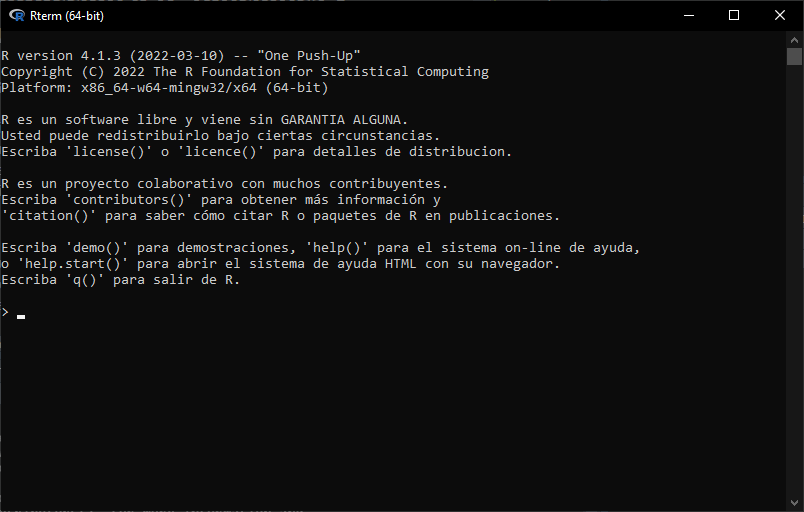
\includegraphics{chapters/images/paste-AC4C7ACA.png}

}

\end{figure}

Un lenguaje de programación interactúa con el usuario, generalmente, a
través de una consola, en donde el usuario ingresa ciertas ``ordenes''
al lenguaje, y éste devuelve un resultado. El ejemplo más sencillo es si
usáramos R como una calculadora.

\begin{Shaded}
\begin{Highlighting}[]
\DecValTok{4} \SpecialCharTok{+} \DecValTok{4}
\end{Highlighting}
\end{Shaded}

\begin{verbatim}
[1] 8
\end{verbatim}

Como puede apreciarse, yo envío una orden a R: que sume 2 + 2, y éste me
devuelve el resultado. Además de esto, podría haber almacenado dicho
resultado dentro de un objeto. Los objetos en R son básicamente
elementos que guardan información que nosotros les depositamos dentro, y
que tenemos que darles un nombre para luego referirnos a ellos. Por
ejemplo, guardaré el resultado de esta suma dentro de un objeto que se
llame ``resultado\_suma''.

\begin{Shaded}
\begin{Highlighting}[]
\NormalTok{resultado\_suma }\OtherTok{\textless{}{-}} \DecValTok{2} \SpecialCharTok{+} \DecValTok{2}
\end{Highlighting}
\end{Shaded}

Varias cosas: para empezar, puede apreciarse que para asignar un
resultado a un objeto, debemos utilizar el ``\textbf{\textless-}'', o
\emph{asignador}. Esto refiere a que básicamente todo lo que esté a la
derecha del símbolo será almacenado en el objeto de la izquierda. Por
otro lado, ¿por qué usé un guión bajo para nombrar a mi objeto? Es que
\textbf{R no permite espacios en nombres de objetos,} tampoco tildes ni
caracteres especiales fuera de los básicos como el guión bajo. Se
recomienda sustituir los espacios por guiones o mayúsculas. Finalmente
vemos que no ha devuelto nada la consola, eso es porque se ha guardado
el valor correctamente, \textbf{al almacenar valores la consola no
devuelve ningún resultado, para acceder al mismo hay que llamar al
objeto creado.}

\begin{Shaded}
\begin{Highlighting}[]
\NormalTok{resultado\_suma}
\end{Highlighting}
\end{Shaded}

\begin{verbatim}
[1] 4
\end{verbatim}

Finalmente, los objetos en R también inteactúan entre ellos. Podemos
generar distintos objetos y obtener resultados al generar su
interacción. Por ejemplo, a continuación tomaré el objeto ya existente
\emph{resultado\_suma}~y le aplicaré una serie de interacciones.

Primero, veremos cómo R permite seguir interactuando con los objetos
luego de haberlos creado.

\begin{Shaded}
\begin{Highlighting}[]
\NormalTok{resultado\_suma }\SpecialCharTok{+} \DecValTok{10}
\end{Highlighting}
\end{Shaded}

\begin{verbatim}
[1] 14
\end{verbatim}

Estas operaciones pueden almacenarse en un nuevo objeto o reescribir al
anterior. Esto podríamos haberlo hecho si al nuevo objeto lo hubiéramos
llamado \emph{resultado\_suma.} Esta acción habría eliminado el viejo
objeto, siendo suplantado por el nuevo, con un distinto valor.

\begin{Shaded}
\begin{Highlighting}[]
\NormalTok{nuevo\_objeto\_suma }\OtherTok{\textless{}{-}}\NormalTok{ resultado\_suma }\SpecialCharTok{+} \DecValTok{10}
\NormalTok{nuevo\_objeto\_suma}
\end{Highlighting}
\end{Shaded}

\begin{verbatim}
[1] 14
\end{verbatim}

Finalmente, se ve a los objetos interactuar entre ellos. El resultado
podría haberse guardado en un nuevo objeto a su vez.

\begin{Shaded}
\begin{Highlighting}[]
\NormalTok{nuevo\_objeto\_suma }\SpecialCharTok{{-}}\NormalTok{ resultado\_suma}
\end{Highlighting}
\end{Shaded}

\begin{verbatim}
[1] 10
\end{verbatim}

\hypertarget{rstudio-pronto-posit}{%
\section{RStudio (pronto POSIT)}\label{rstudio-pronto-posit}}

Programar vinculándose tan solo con la consola puede ser un poco contra
intuitivo. Felizmente hay herramientas que permiten hacerle la vida más
fácil al analista. En R, sin dudas la más popular es
\href{https://www.rstudio.com/}{RStudio}.

RStudio es el IDE principal de R. Un
\href{https://en.wikipedia.org/wiki/Integrated_development_environment}{IDE}
(Integrated Development Environment) es un programa pensado para
desarrollar software. En este caso, como R es un lenguaje utilizado para
el análisis de datos, está pensado específicamente para este fin.

Algunos IDE sirven para un lenguaje de programación específico, y otros
aceptan varios. El más famoso es
\href{https://code.visualstudio.com/}{VSCode}, de Microsoft, en donde
también se puede usar R, pero no es tan popular dentro de la comunidad.
RStudio admite varios lenguajes de programación además de R, entre ellos
Python, JavaScript y Julia.

Finalmente, RStudio se está convirtiendo en
\href{https://posit.co/}{posit}.

\begin{figure}

{\centering \includegraphics{chapters/images/rstudio2_gy2jzi.webp}

}

\end{figure}

RStudio tiene cuatro grandes secciones, tal como se muestra en la imagen
previa. A continuación se detallarán:

\begin{itemize}
\item
  \textbf{Script:} es el editor de texto dentro de RStudio, es donde se
  escriben los comandos que luego se enviarán a la consola para su
  ejecución. Permite al analista mantener ordenado y documentado todo lo
  que ha hecho en R y puede guardarse para luego o enviarse como
  cualquier documento. Es el principal socio del analista y puede
  trabajarse con varios a la vez. Por lo general, cuando abrimos RStudio
  no aparece, se debe abrir uno nuevo.
\item
  \textbf{Consola:} es donde R efectivamente trabaja y ejecuta los
  comandos que se le van enviando. Vendría a ser lo utilizado en el
  módulo anterior insertado dentro de una herramienta que permite más
  funciones.
\item
  \textbf{Enviroment:} es el listado de objetos que se van creando en R.
  En el caso de los ejemplos anteriores, aparecerían listados
  \emph{resultado\_suma} y \emph{nuevo objeto\_suma.} También aparecen
  los dataframes y las funciones creadas por el usuario.
\item
  \textbf{Output:} esta pestaña sirve para varias cuestiones. Para
  empezar, muestra los gráficos generados en R, tal como aparece en la
  imagen, pero también permite ver los archivos del proyecto de R, y los
  paquetes. También, cuando se requiera, aparecerá la documentación de
  ayuda de las funciones utilizadas.
\end{itemize}

\hypertarget{funciones}{%
\section{Funciones}\label{funciones}}

En R se programa. Aprender a programar es un proceso de largo aliento,
no es como una suite de bussines analytics como Power BI.\footnote{Ver
  artículo:
  \href{https://www.linkedin.com/pulse/la-santa-trinidad-del-an\%25C3\%25A1lisis-de-datos-daniel-blanc/?trackingId=gthGpbnJTJWapZz79uRNlQ\%3D\%3D}{La
  santa trinidad del análisis de datos}} Puede llevar meses sentirse a
gusto con la programación. Lo fundamental es la práctica. Felizmente, no
necesitamos ser expertos en programación para realizar análisis de
datos.

Una librería es una serie de funciones que podemos descargar y utilizar
para llevar a cabo nuestros propósitos en R (por ejemplo, importar un
archivo con datos).

Y\ldots{} qué es una función?

Una función es un bloque de código que permite que realice determinada
acción.

\begin{Shaded}
\begin{Highlighting}[]
\NormalTok{mi\_funcion }\OtherTok{\textless{}{-}} \ControlFlowTok{function}\NormalTok{() \{ }
  \FunctionTok{print}\NormalTok{(}\StringTok{"Hola chiques!"}\NormalTok{)}
\NormalTok{\}}
\end{Highlighting}
\end{Shaded}

\hypertarget{boom}{%
\section{BOOM!}\label{boom}}

\begin{Shaded}
\begin{Highlighting}[]
\FunctionTok{mi\_funcion}\NormalTok{()}
\end{Highlighting}
\end{Shaded}

\begin{verbatim}
[1] "Hola chiques!"
\end{verbatim}

\hypertarget{paruxe1metros}{%
\section{Parámetros}\label{paruxe1metros}}

Los parámetros son valores que se sustituirán por aquellos que
necesitemos al llamar a la función.

\begin{Shaded}
\begin{Highlighting}[]
\NormalTok{nombre\_completo }\OtherTok{\textless{}{-}} \ControlFlowTok{function}\NormalTok{(nombre, apellido) \{}
  \FunctionTok{paste}\NormalTok{(nombre, apellido)}
\NormalTok{\}}
\end{Highlighting}
\end{Shaded}

Suelen tener nombres que explicitan lo que hacen.

\begin{Shaded}
\begin{Highlighting}[]
\FunctionTok{nombre\_completo}\NormalTok{(}\StringTok{"Homero"}\NormalTok{, }\StringTok{"Simpson"}\NormalTok{)}
\end{Highlighting}
\end{Shaded}

\begin{verbatim}
[1] "Homero Simpson"
\end{verbatim}

\hypertarget{tuya-huxe9ctor}{%
\section{Tuya Héctor!}\label{tuya-huxe9ctor}}

Ahora les toca a ustedes:

Cree una función que tome dos números y devuelva la suma de ambos.

Cree una función que tome tres valores:

\begin{itemize}
\item
  Dos serán números
\item
  Y el tercero será la operación que querrá que ocurra entre los otros
  dos valores ingresados.
\item
  Debe poder: sumar, restar y multiplicar.
\item
  Debe realizar la operación solicitada y devolver el valor
\item
  Conviene googlear sobre condicionales en R ;)
\end{itemize}

\hypertarget{posibles-soluciones}{%
\section{Posibles soluciones}\label{posibles-soluciones}}

\begin{Shaded}
\begin{Highlighting}[]
\NormalTok{suma }\OtherTok{\textless{}{-}} \ControlFlowTok{function}\NormalTok{(numero\_1, numero\_2)\{}
  \FunctionTok{return}\NormalTok{(numero\_1 }\SpecialCharTok{+}\NormalTok{ numero\_2)}
\NormalTok{\}}

\FunctionTok{suma}\NormalTok{(}\DecValTok{250}\NormalTok{,}\DecValTok{50}\NormalTok{)}

\NormalTok{operacion }\OtherTok{\textless{}{-}} \ControlFlowTok{function}\NormalTok{(numero\_1, numero\_2, operacion)\{}
  \ControlFlowTok{if}\NormalTok{ (operacion }\SpecialCharTok{==} \StringTok{"sumar"}\NormalTok{)\{}
    \FunctionTok{return}\NormalTok{(numero\_1 }\SpecialCharTok{+}\NormalTok{ numero\_2)}
\NormalTok{  \} }\ControlFlowTok{else} \ControlFlowTok{if}\NormalTok{ (operacion }\SpecialCharTok{==} \StringTok{"restar"}\NormalTok{)\{}
    \FunctionTok{return}\NormalTok{(numero\_1 }\SpecialCharTok{{-}}\NormalTok{ numero\_2)}
\NormalTok{  \} }\ControlFlowTok{else} \ControlFlowTok{if}\NormalTok{ (operacion }\SpecialCharTok{==} \StringTok{"multiplicar"}\NormalTok{)\{}
    \FunctionTok{return}\NormalTok{(numero\_1 }\SpecialCharTok{*}\NormalTok{ numero\_2)}
\NormalTok{  \} }\ControlFlowTok{else}\NormalTok{ \{}
    \FunctionTok{return}\NormalTok{(}\StringTok{"Error"}\NormalTok{)}
\NormalTok{  \}}
\NormalTok{\}}

\FunctionTok{operacion}\NormalTok{(}\DecValTok{10}\NormalTok{,}\DecValTok{5}\NormalTok{, }\StringTok{"sumar"}\NormalTok{)}
\FunctionTok{operacion}\NormalTok{(}\DecValTok{10}\NormalTok{,}\DecValTok{5}\NormalTok{, }\StringTok{"restar"}\NormalTok{)}
\FunctionTok{operacion}\NormalTok{(}\DecValTok{10}\NormalTok{,}\DecValTok{5}\NormalTok{, }\StringTok{"multiplicar"}\NormalTok{)}
\FunctionTok{operacion}\NormalTok{(}\DecValTok{10}\NormalTok{,}\DecValTok{5}\NormalTok{, }\StringTok{"dividir"}\NormalTok{)}
\end{Highlighting}
\end{Shaded}

\bookmarksetup{startatroot}

\hypertarget{importaciuxf3n-de-datos}{%
\chapter{Importación de datos}\label{importaciuxf3n-de-datos}}

Daniel Blanc

\hfill\break

\hypertarget{funciones-buxe1sicas}{%
\subsection{Funciones básicas}\label{funciones-buxe1sicas}}

Cuando trabajamos con archivos de texto plano, lo mejor que podemos
hacer cuando pensamos en importarlo, es abrirlo con un bloc de notas (en
la medida que el tamaño lo permita).

La función más elemental para importar archivos de texto plano es
\emph{read.table.} Esta función tiene la particularidad que
prácticamente no toma ningun valor por defecto en sus parámetros y hay
que rellenarlos todos de modo de generar una importación.

\begin{Shaded}
\begin{Highlighting}[]
\NormalTok{data }\OtherTok{\textless{}{-}} \FunctionTok{read.table}\NormalTok{(}\StringTok{"../data/courseid\_3282\_participants.csv"}\NormalTok{)}
\NormalTok{data}
\end{Highlighting}
\end{Shaded}

La sentencia ejecutada anteriormente da el siguiente error:

\begin{quote}
Error in scan(file = file, what = what, sep = sep, quote = quote, dec =
dec, : line 2 did not have 3 elements
\end{quote}

Esto ocurre porque read.table no sabe qué hacer en el caso de que una
fila no contenga el mismo número de elementos que el resto. Para
solucionar esto podemos agregar el parámetro que lo aclare.

\begin{Shaded}
\begin{Highlighting}[]
\NormalTok{data }\OtherTok{\textless{}{-}} \FunctionTok{read.table}\NormalTok{(}\StringTok{"../data/courseid\_3282\_participants.csv"}\NormalTok{, }\AttributeTok{fill =} \ConstantTok{NA}\NormalTok{)}
\end{Highlighting}
\end{Shaded}

\begin{longtable}[]{@{}lll@{}}
\toprule()
V1 & V2 & V3 \\
\midrule()
\endhead
Nombre,Apellido(s),``Dirección & de & correo'' \\
CECILIA,CARPENA,mcarpena@msp.gub.uy & & \\
Marines,FIGUEROA,mfigueroa@msp.gub.uy & & \\
LUCA,AICARDI,maicardi@msp.gub.uy & & \\
MARCELA,CASTRO,mfcastro@msp.gub.uy & & \\
MARIA,MORATORIO,xmoratorio@msp.gub.uy & & \\
\bottomrule()
\end{longtable}

\textbf{Tenemos la tabla!} Aunque, realmente no es lo que esperábamos.
Para empezar, los nombres de las columnas no son correctos. Parece ser
que read.table por defecto no se da cuenta que la primera fila
corresponde a los encabezados de la tabla. Vamos a tener que aclarárselo
también.

\begin{Shaded}
\begin{Highlighting}[]
\NormalTok{data }\OtherTok{\textless{}{-}} \FunctionTok{read.table}\NormalTok{(}
  \AttributeTok{file =} \StringTok{"../data/courseid\_3282\_participants.csv"}\NormalTok{, }
  \AttributeTok{fill =} \ConstantTok{NA}\NormalTok{,}
  \AttributeTok{header =} \ConstantTok{TRUE}
\NormalTok{)}
\end{Highlighting}
\end{Shaded}

\begin{longtable}[]{@{}lll@{}}
\toprule()
Nombre.Apellido.s\ldots Dirección & de & correo. \\
\midrule()
\endhead
CECILIA,CARPENA,mcarpena@msp.gub.uy & NA & NA \\
Marines,FIGUEROA,mfigueroa@msp.gub.uy & NA & NA \\
LUCA,AICARDI,maicardi@msp.gub.uy & NA & NA \\
MARCELA,CASTRO,mfcastro@msp.gub.uy & NA & NA \\
MARIA,MORATORIO,xmoratorio@msp.gub.uy & NA & NA \\
Daniel,BLANC,dblanc@ine.gub.uy & NA & NA \\
\bottomrule()
\end{longtable}

\textbf{Corregimos los encabezados!} Pero aún parece que hay problemas:
notoriamente esta tabla debería tener tres columnas: nombre, apellido y
dirección de correo. Pero esto no ocurre.

El problema radica en que read.table toma por defecto que el separador
de los datos es un espacio en blanco. Es por esto que dirección de
correo está separado como si fueran tres columnas. Debemos especificarle
cuál es el separador correcto: la coma.

\begin{Shaded}
\begin{Highlighting}[]
\NormalTok{data }\OtherTok{\textless{}{-}} \FunctionTok{read.table}\NormalTok{(}
  \AttributeTok{file =} \StringTok{"../data/courseid\_3282\_participants.csv"}\NormalTok{, }
  \AttributeTok{fill =} \ConstantTok{NA}\NormalTok{,}
  \AttributeTok{header =} \ConstantTok{TRUE}\NormalTok{,}
  \AttributeTok{sep =} \StringTok{","}
\NormalTok{)}
\end{Highlighting}
\end{Shaded}

\begin{longtable}[]{@{}lll@{}}
\toprule()
Nombre & Apellido.s. & Dirección.de.correo \\
\midrule()
\endhead
CECILIA & CARPENA & mcarpena@msp.gub.uy \\
Marines & FIGUEROA & mfigueroa@msp.gub.uy \\
LUCA & AICARDI & maicardi@msp.gub.uy \\
MARCELA & CASTRO & mfcastro@msp.gub.uy \\
MARIA & MORATORIO & xmoratorio@msp.gub.uy \\
Daniel & BLANC & dblanc@ine.gub.uy \\
\bottomrule()
\end{longtable}

\textbf{Ya casi es nuestra tabla!} Pero siguen habiendo cuestiones a
pulir, y es que parece haber algún problema con los caracteres
especiales, tales como los paréntesis o tildes. Podemos solucionar esto
especificando el tipo de encoding que tiene el archivo. Para descubrir
el mismo, debemos mirar en la parte inferior derecha del archivo de
texto plano.

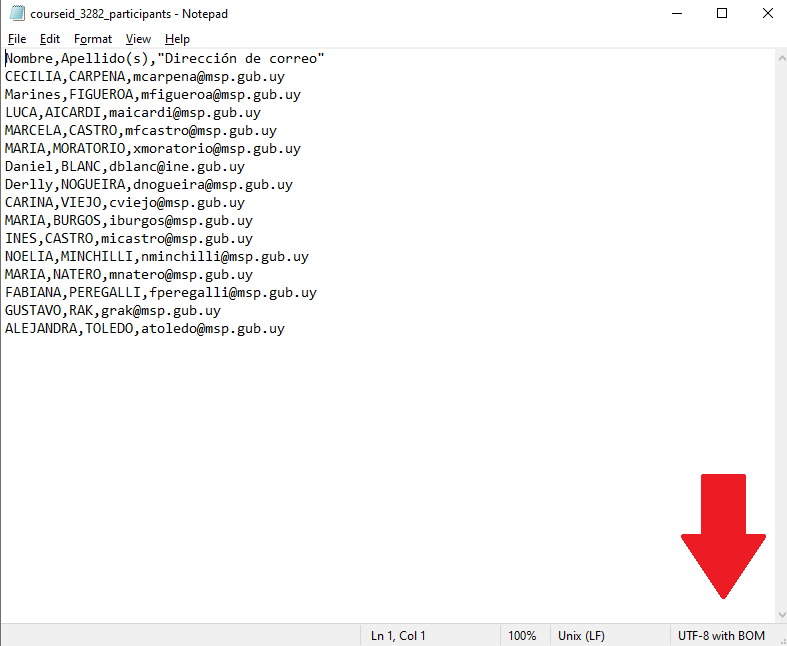
\includegraphics{chapters/images/encoding_2.png}

\begin{Shaded}
\begin{Highlighting}[]
\NormalTok{data }\OtherTok{\textless{}{-}} \FunctionTok{read.table}\NormalTok{(}
  \AttributeTok{file =} \StringTok{"../data/courseid\_3282\_participants.csv"}\NormalTok{, }
  \AttributeTok{fill =} \ConstantTok{NA}\NormalTok{,}
  \AttributeTok{header =} \ConstantTok{TRUE}\NormalTok{,}
  \AttributeTok{sep =} \StringTok{","}\NormalTok{,}
  \AttributeTok{fileEncoding =} \StringTok{\textquotesingle{}UTF{-}8{-}BOM\textquotesingle{}}
\NormalTok{)}
\end{Highlighting}
\end{Shaded}

\begin{longtable}[]{@{}lll@{}}
\toprule()
Nombre & Apellido.s. & Dirección.de.correo \\
\midrule()
\endhead
CECILIA & CARPENA & mcarpena@msp.gub.uy \\
Marines & FIGUEROA & mfigueroa@msp.gub.uy \\
LUCA & AICARDI & maicardi@msp.gub.uy \\
MARCELA & CASTRO & mfcastro@msp.gub.uy \\
MARIA & MORATORIO & xmoratorio@msp.gub.uy \\
Daniel & BLANC & dblanc@ine.gub.uy \\
\bottomrule()
\end{longtable}

\textbf{Ahora si tenemos nuestra tabla!} R no es amigo de los caracteres
especiales de ningún tipo. Está pensado para nombres funcionales e
informáticos, no para humanos. Por tanto, conviene darles los nombres
que nosotros queremos a los encabezados.

\begin{Shaded}
\begin{Highlighting}[]
\NormalTok{data }\OtherTok{\textless{}{-}} \FunctionTok{read.table}\NormalTok{(}
  \AttributeTok{file =} \StringTok{"../data/courseid\_3282\_participants.csv"}\NormalTok{, }
  \AttributeTok{fill =} \ConstantTok{NA}\NormalTok{,}
  \AttributeTok{header =} \ConstantTok{TRUE}\NormalTok{,}
  \AttributeTok{sep =} \StringTok{","}\NormalTok{,}
  \AttributeTok{fileEncoding =} \StringTok{\textquotesingle{}UTF{-}8{-}BOM\textquotesingle{}}\NormalTok{,}
  \AttributeTok{col.names =} \FunctionTok{c}\NormalTok{(}\StringTok{\textquotesingle{}nombre\textquotesingle{}}\NormalTok{, }\StringTok{\textquotesingle{}apellido\textquotesingle{}}\NormalTok{, }\StringTok{\textquotesingle{}direccion\_correo\textquotesingle{}}\NormalTok{)}
\NormalTok{)}
\end{Highlighting}
\end{Shaded}

\begin{longtable}[]{@{}lll@{}}
\toprule()
nombre & apellido & direccion\_correo \\
\midrule()
\endhead
CECILIA & CARPENA & mcarpena@msp.gub.uy \\
Marines & FIGUEROA & mfigueroa@msp.gub.uy \\
LUCA & AICARDI & maicardi@msp.gub.uy \\
MARCELA & CASTRO & mfcastro@msp.gub.uy \\
MARIA & MORATORIO & xmoratorio@msp.gub.uy \\
Daniel & BLANC & dblanc@ine.gub.uy \\
\bottomrule()
\end{longtable}

Como se ha visto, para importar una tabla de texto plano en R se deben
tomar en cuenta los siguientes elementos:

\begin{itemize}
\item
  Si el archivo tiene encabezados
\item
  Cuál es el separador de los datos
\item
  Si hay que rellenar espacios en blancos con NA
\item
  El encoding del archivo
\end{itemize}

Lo cierto es que \emph{read.table} es la versión más básica de una serie
de funciones que sirven para el mismo propósito. Si ya conocemos de
antemano el formato en que viene nuestro dataset, podemos usar funciones
que requieran menos trabajo para obtener la información.

Por ejemplo, si sabemos que nuestro archivo es un csv, podemos usar la
función \emph{read.csv}. Esta función ya da por hecho que el dataset
contiene los encabezados en la primera fila y que el separador es una
coma. Para alcanzar el mismo resultado que antes, solo debemos aclararle
el encoding y el nombre que queremos para las columnas.

\begin{Shaded}
\begin{Highlighting}[]
\NormalTok{data }\OtherTok{\textless{}{-}} \FunctionTok{read.csv}\NormalTok{(}
  \AttributeTok{file =} \StringTok{"../data/courseid\_3282\_participants.csv"}\NormalTok{,}
  \AttributeTok{fileEncoding =} \StringTok{\textquotesingle{}UTF{-}8{-}BOM\textquotesingle{}}\NormalTok{,}
  \AttributeTok{col.names =} \FunctionTok{c}\NormalTok{(}\StringTok{\textquotesingle{}nombre\textquotesingle{}}\NormalTok{, }\StringTok{\textquotesingle{}apellido\textquotesingle{}}\NormalTok{, }\StringTok{\textquotesingle{}direccion\_correo\textquotesingle{}}\NormalTok{)}
\NormalTok{)}
\end{Highlighting}
\end{Shaded}

\begin{longtable}[]{@{}lll@{}}
\toprule()
nombre & apellido & direccion\_correo \\
\midrule()
\endhead
CECILIA & CARPENA & mcarpena@msp.gub.uy \\
Marines & FIGUEROA & mfigueroa@msp.gub.uy \\
LUCA & AICARDI & maicardi@msp.gub.uy \\
MARCELA & CASTRO & mfcastro@msp.gub.uy \\
MARIA & MORATORIO & xmoratorio@msp.gub.uy \\
Daniel & BLANC & dblanc@ine.gub.uy \\
\bottomrule()
\end{longtable}

\begin{quote}
Tomar en cuenta que tanto \emph{read.csv, read.csv2, read.delim}, entre
muchas otras funciones, son de la misma ``familia'' que
\emph{read.table}. Funcionan prácticamente igual solo que cambian los
parámetros por defecto.
\end{quote}

Lo devuelto por estas funciones, es un \textbf{\emph{data frame}}, lo
cual es un objeto computacional diseñado para almacenar datos con forma
de tabla.

\hypertarget{funciones-inteligentes}{%
\subsection{Funciones inteligentes}\label{funciones-inteligentes}}

Adicionalmente, el paquete
\href{https://www.rdocumentation.org/packages/data.table/versions/1.14.2}{\emph{data.table}},
tiene una función llamada
\href{https://www.rdocumentation.org/packages/data.table/versions/1.14.2/topics/fread}{\emph{fread}}
que permite no solo ser más eficiente con la lectura de los datos, sino
que no requiere especificación de separador.

\begin{Shaded}
\begin{Highlighting}[]
\FunctionTok{library}\NormalTok{(data.table)}
\NormalTok{data }\OtherTok{\textless{}{-}} \FunctionTok{fread}\NormalTok{(}\StringTok{"../data/courseid\_3282\_participants.csv"}\NormalTok{)}
\end{Highlighting}
\end{Shaded}

\begin{longtable}[]{@{}lll@{}}
\toprule()
Nombre & Apellido(s) & Dirección de correo \\
\midrule()
\endhead
CECILIA & CARPENA & mcarpena@msp.gub.uy \\
Marines & FIGUEROA & mfigueroa@msp.gub.uy \\
LUCA & AICARDI & maicardi@msp.gub.uy \\
MARCELA & CASTRO & mfcastro@msp.gub.uy \\
MARIA & MORATORIO & xmoratorio@msp.gub.uy \\
Daniel & BLANC & dblanc@ine.gub.uy \\
\bottomrule()
\end{longtable}

El único inconveniente parece ser el encoding, pero aclarándoselo, la
función nos trae la información perfectamente.

\begin{Shaded}
\begin{Highlighting}[]
\NormalTok{data }\OtherTok{\textless{}{-}} \FunctionTok{fread}\NormalTok{(}
  \AttributeTok{file =} \StringTok{"../data/courseid\_3282\_participants.csv"}\NormalTok{,}
  \AttributeTok{encoding =} \StringTok{"UTF{-}8"}
\NormalTok{)}
\end{Highlighting}
\end{Shaded}

\begin{longtable}[]{@{}lll@{}}
\toprule()
Nombre & Apellido(s) & Dirección de correo \\
\midrule()
\endhead
CECILIA & CARPENA & mcarpena@msp.gub.uy \\
Marines & FIGUEROA & mfigueroa@msp.gub.uy \\
LUCA & AICARDI & maicardi@msp.gub.uy \\
MARCELA & CASTRO & mfcastro@msp.gub.uy \\
MARIA & MORATORIO & xmoratorio@msp.gub.uy \\
Daniel & BLANC & dblanc@ine.gub.uy \\
\bottomrule()
\end{longtable}

\hypertarget{funciones-muxe1s-eficientes}{%
\subsection{Funciones más
eficientes}\label{funciones-muxe1s-eficientes}}

Hay un paquete en R especializado en la lectura de archivos. Ese paquete
se llama
\href{https://www.rdocumentation.org/packages/readr/versions/2.1.2}{\emph{readr}}\emph{.}
El objetivo de este paquete es realizar una importación de datos más
veloz y eficiente. Además, nos ahorra tiempo en la medida que detecta
automáticamente el separador de los datos.

\begin{Shaded}
\begin{Highlighting}[]
\FunctionTok{library}\NormalTok{(readr)}
\NormalTok{data }\OtherTok{\textless{}{-}} \FunctionTok{read\_csv}\NormalTok{(}\StringTok{"../data/courseid\_3282\_participants.csv"}\NormalTok{)}
\end{Highlighting}
\end{Shaded}

\begin{verbatim}
Rows: 15 Columns: 3
-- Column specification --------------------------------------------------------
Delimiter: ","
chr (3): Nombre, Apellido(s), Dirección de correo

i Use `spec()` to retrieve the full column specification for this data.
i Specify the column types or set `show_col_types = FALSE` to quiet this message.
\end{verbatim}

\begin{longtable}[]{@{}lll@{}}
\toprule()
Nombre & Apellido(s) & Dirección de correo \\
\midrule()
\endhead
CECILIA & CARPENA & mcarpena@msp.gub.uy \\
Marines & FIGUEROA & mfigueroa@msp.gub.uy \\
LUCA & AICARDI & maicardi@msp.gub.uy \\
MARCELA & CASTRO & mfcastro@msp.gub.uy \\
MARIA & MORATORIO & xmoratorio@msp.gub.uy \\
Daniel & BLANC & dblanc@ine.gub.uy \\
\bottomrule()
\end{longtable}

Esta función no solo lee la información con mayor velocidad, sino que
también es más inteligente a la hora de resolver la cuestión del
encoding y el problema de los nombres de las columnas. También nos
brinda información sobre el dataset, como la cantidad de filas,
columnas, y el tipo de dato de ellas. Podemos acceder a mayor
información sobre esto último su complementamos con la función spec.

\begin{Shaded}
\begin{Highlighting}[]
\FunctionTok{spec}\NormalTok{(data)}
\end{Highlighting}
\end{Shaded}

\begin{verbatim}
cols(
  Nombre = col_character(),
  `Apellido(s)` = col_character(),
  `Dirección de correo` = col_character()
)
\end{verbatim}

El paquete readr permite también editar el tipo de las columnas en el
momento que se realiza la importación. De este modo, si tenemos que
hacer un cambio de tipo de dato, podemos hacerlo integrado a la función,
sin tener que dedicar tiempo a eso después.

\begin{Shaded}
\begin{Highlighting}[]
\NormalTok{data }\OtherTok{\textless{}{-}} \FunctionTok{read\_csv}\NormalTok{(}
  \AttributeTok{file =} \StringTok{"../data/courseid\_3282\_participants.csv"}\NormalTok{,}
  \AttributeTok{col\_names =} \FunctionTok{c}\NormalTok{(}\StringTok{"nombre"}\NormalTok{, }\StringTok{"apellido"}\NormalTok{, }\StringTok{"direccion\_correo"}\NormalTok{),}
  \AttributeTok{col\_types =} \FunctionTok{cols}\NormalTok{(}
    \AttributeTok{nombre =} \FunctionTok{col\_character}\NormalTok{(),}
    \AttributeTok{apellido =} \FunctionTok{col\_character}\NormalTok{(),}
    \AttributeTok{direccion\_correo =} \FunctionTok{col\_character}\NormalTok{()}
\NormalTok{  )}
\NormalTok{)}
\end{Highlighting}
\end{Shaded}

\begin{longtable}[]{@{}lll@{}}
\toprule()
nombre & apellido & direccion\_correo \\
\midrule()
\endhead
Nombre & Apellido(s) & Dirección de correo \\
CECILIA & CARPENA & mcarpena@msp.gub.uy \\
Marines & FIGUEROA & mfigueroa@msp.gub.uy \\
LUCA & AICARDI & maicardi@msp.gub.uy \\
MARCELA & CASTRO & mfcastro@msp.gub.uy \\
MARIA & MORATORIO & xmoratorio@msp.gub.uy \\
\bottomrule()
\end{longtable}

\begin{quote}
Como notarán, antes de asignarle un tipo de dato a las columnas, les
asigné el nombre, de modo que R supiera a cuál me estaba refieriendo en
cada caso. A veces cuando los encabezados tienen espacios o tildes, o
cuestiones de ese estilo, y no son solo letras y guiones, R puede
asignarles nombres inesperados.
\end{quote}

Sin embargo, esto nos trajo un problema, ya que parece que \emph{readr}
entiende que si le ponemos nombres a las columnas, es que en realidad no
tienen nombres, y la primera fila son datos y no encabezados. Por tanto,
para solucionar esto debemos pedirle que omita la primera fila. Para
ello, se usa el parámetro \emph{skip}.

\begin{Shaded}
\begin{Highlighting}[]
\NormalTok{data }\OtherTok{\textless{}{-}} \FunctionTok{read\_csv}\NormalTok{(}
  \AttributeTok{file =} \StringTok{"../data/courseid\_3282\_participants.csv"}\NormalTok{,}
  \AttributeTok{col\_names =} \FunctionTok{c}\NormalTok{(}\StringTok{"nombre"}\NormalTok{, }\StringTok{"apellido"}\NormalTok{, }\StringTok{"direccion\_correo"}\NormalTok{),}
  \AttributeTok{col\_types =} \FunctionTok{cols}\NormalTok{(}
    \AttributeTok{nombre =} \FunctionTok{col\_character}\NormalTok{(),}
    \AttributeTok{apellido =} \FunctionTok{col\_character}\NormalTok{(),}
    \AttributeTok{direccion\_correo =} \FunctionTok{col\_character}\NormalTok{()}
\NormalTok{  ),}
  \AttributeTok{skip =} \DecValTok{1}
\NormalTok{)}
\end{Highlighting}
\end{Shaded}

\begin{longtable}[]{@{}lll@{}}
\toprule()
nombre & apellido & direccion\_correo \\
\midrule()
\endhead
CECILIA & CARPENA & mcarpena@msp.gub.uy \\
Marines & FIGUEROA & mfigueroa@msp.gub.uy \\
LUCA & AICARDI & maicardi@msp.gub.uy \\
MARCELA & CASTRO & mfcastro@msp.gub.uy \\
MARIA & MORATORIO & xmoratorio@msp.gub.uy \\
Daniel & BLANC & dblanc@ine.gub.uy \\
\bottomrule()
\end{longtable}

\hypertarget{archivos-de-excel}{%
\section{Archivos de excel}\label{archivos-de-excel}}

Excel es otro clásico modo de almacenar información, aunque no en
grandes volúmenes. Para poder leer información de esta fuente, se puede
recurrir al paquete
\href{https://www.rdocumentation.org/packages/openxlsx/versions/4.2.5}{\emph{openxlsx}}.

\begin{Shaded}
\begin{Highlighting}[]
\FunctionTok{library}\NormalTok{(openxlsx)}
\NormalTok{data }\OtherTok{\textless{}{-}} \FunctionTok{read.xlsx}\NormalTok{(}\StringTok{"../data/ACV EFMA 2022.xlsx"}\NormalTok{)}
\end{Highlighting}
\end{Shaded}

\begin{longtable}[]{@{}
  >{\raggedleft\arraybackslash}p{(\columnwidth - 10\tabcolsep) * \real{0.0875}}
  >{\raggedright\arraybackslash}p{(\columnwidth - 10\tabcolsep) * \real{0.1500}}
  >{\raggedright\arraybackslash}p{(\columnwidth - 10\tabcolsep) * \real{0.0625}}
  >{\raggedleft\arraybackslash}p{(\columnwidth - 10\tabcolsep) * \real{0.2500}}
  >{\raggedleft\arraybackslash}p{(\columnwidth - 10\tabcolsep) * \real{0.1250}}
  >{\raggedright\arraybackslash}p{(\columnwidth - 10\tabcolsep) * \real{0.3250}}@{}}
\toprule()
\begin{minipage}[b]{\linewidth}\raggedleft
Codigo
\end{minipage} & \begin{minipage}[b]{\linewidth}\raggedright
Institucion
\end{minipage} & \begin{minipage}[b]{\linewidth}\raggedright
Sexo
\end{minipage} & \begin{minipage}[b]{\linewidth}\raggedleft
Fecha.de.nacimiento
\end{minipage} & \begin{minipage}[b]{\linewidth}\raggedleft
Fecha.ACV
\end{minipage} & \begin{minipage}[b]{\linewidth}\raggedright
Trombolisis.medicamentosa
\end{minipage} \\
\midrule()
\endhead
138 & AMDM & M & 15014 & 44565 & NO \\
138 & AMDM & M & 21693 & 44565 & NO \\
138 & AMDM & M & 16604 & 44566 & NO \\
138 & AMDM & M & 21545 & 44567 & NO \\
138 & AMDM & F & 19542 & 44568 & NO \\
138 & AMDM & F & 17541 & 44570 & NO \\
\bottomrule()
\end{longtable}

\begin{quote}
Obtener datos desde excel por lo general requiere poco trabajo, ya que
la información está delimitada en las propias celdas de excel y no
tenemos que aclararle mucho a la función. Lo único que nos puede dar
problema es la cuestión del \textbf{formato de las fechas}, ya que excel
almacena las fechas como números enteros.
\end{quote}

Para evitar que esto suceda, debemos utilizar el parámetro
correspondiente: detectDates.

\begin{Shaded}
\begin{Highlighting}[]
\NormalTok{data }\OtherTok{\textless{}{-}} \FunctionTok{read.xlsx}\NormalTok{(}
  \AttributeTok{xlsxFile =} \StringTok{"../data/ACV EFMA 2022.xlsx"}\NormalTok{,}
  \AttributeTok{detectDates =} \ConstantTok{TRUE}
\NormalTok{)}
\end{Highlighting}
\end{Shaded}

\begin{longtable}[]{@{}
  >{\raggedleft\arraybackslash}p{(\columnwidth - 10\tabcolsep) * \real{0.0864}}
  >{\raggedright\arraybackslash}p{(\columnwidth - 10\tabcolsep) * \real{0.1481}}
  >{\raggedright\arraybackslash}p{(\columnwidth - 10\tabcolsep) * \real{0.0617}}
  >{\raggedright\arraybackslash}p{(\columnwidth - 10\tabcolsep) * \real{0.2469}}
  >{\raggedright\arraybackslash}p{(\columnwidth - 10\tabcolsep) * \real{0.1358}}
  >{\raggedright\arraybackslash}p{(\columnwidth - 10\tabcolsep) * \real{0.3210}}@{}}
\toprule()
\begin{minipage}[b]{\linewidth}\raggedleft
Codigo
\end{minipage} & \begin{minipage}[b]{\linewidth}\raggedright
Institucion
\end{minipage} & \begin{minipage}[b]{\linewidth}\raggedright
Sexo
\end{minipage} & \begin{minipage}[b]{\linewidth}\raggedright
Fecha.de.nacimiento
\end{minipage} & \begin{minipage}[b]{\linewidth}\raggedright
Fecha.ACV
\end{minipage} & \begin{minipage}[b]{\linewidth}\raggedright
Trombolisis.medicamentosa
\end{minipage} \\
\midrule()
\endhead
138 & AMDM & M & 1941-02-07 & 2022-01-04 & NO \\
138 & AMDM & M & 1959-05-23 & 2022-01-04 & NO \\
138 & AMDM & M & 1945-06-16 & 2022-01-05 & NO \\
138 & AMDM & M & 1958-12-26 & 2022-01-06 & NO \\
138 & AMDM & F & 1953-07-02 & 2022-01-07 & NO \\
138 & AMDM & F & 1948-01-09 & 2022-01-09 & NO \\
\bottomrule()
\end{longtable}

También se puede seleccionar de qué hoja del libro hacer la lectura,
entre otras cuestiones. Para seleccionar la hoja, se puede poner tanto
el nombre de la hoja, como el número.

\begin{Shaded}
\begin{Highlighting}[]
\NormalTok{data }\OtherTok{\textless{}{-}} \FunctionTok{read.xlsx}\NormalTok{(}
  \AttributeTok{xlsxFile =} \StringTok{"../data/ACV EFMA 2022.xlsx"}\NormalTok{,}
  \AttributeTok{detectDates =} \ConstantTok{TRUE}\NormalTok{,}
  \AttributeTok{sheet =} \DecValTok{2}
\NormalTok{)}
\end{Highlighting}
\end{Shaded}

\begin{longtable}[]{@{}lll@{}}
\toprule()
Nombre & Apellido(s) & Dirección.de.correo \\
\midrule()
\endhead
CECILIA & CARPENA & mcarpena@msp.gub.uy \\
Marines & FIGUEROA & mfigueroa@msp.gub.uy \\
LUCA & AICARDI & maicardi@msp.gub.uy \\
MARCELA & CASTRO & mfcastro@msp.gub.uy \\
MARIA & MORATORIO & xmoratorio@msp.gub.uy \\
Daniel & BLANC & dblanc@ine.gub.uy \\
\bottomrule()
\end{longtable}

\hypertarget{archivos-de-spss}{%
\section{Archivos de SPSS}\label{archivos-de-spss}}

Es muy común migrar de SPSS a R, y por tanto, hay un paquete que tenemos
que tener presente para acceder a archivos creados a partir de esa
herramienta, y es el
\href{https://www.rdocumentation.org/packages/haven/versions/2.5.0}{\emph{haven}}.
Dentro de ese paquete, tenemos una función denominada \emph{read\_sav},
que sirve para acceder a acceder a archivos de este estilo.

\begin{Shaded}
\begin{Highlighting}[]
\FunctionTok{library}\NormalTok{(haven)}
\NormalTok{data }\OtherTok{\textless{}{-}} \FunctionTok{read\_sav}\NormalTok{(}\StringTok{"../data/Natalidad2021\_ENAP\_CursoR.sav"}\NormalTok{)}
\end{Highlighting}
\end{Shaded}

\begin{longtable}[]{@{}
  >{\raggedleft\arraybackslash}p{(\columnwidth - 34\tabcolsep) * \real{0.0448}}
  >{\raggedleft\arraybackslash}p{(\columnwidth - 34\tabcolsep) * \real{0.0448}}
  >{\raggedleft\arraybackslash}p{(\columnwidth - 34\tabcolsep) * \real{0.0448}}
  >{\raggedleft\arraybackslash}p{(\columnwidth - 34\tabcolsep) * \real{0.0448}}
  >{\raggedleft\arraybackslash}p{(\columnwidth - 34\tabcolsep) * \real{0.0672}}
  >{\raggedleft\arraybackslash}p{(\columnwidth - 34\tabcolsep) * \real{0.0597}}
  >{\raggedleft\arraybackslash}p{(\columnwidth - 34\tabcolsep) * \real{0.0597}}
  >{\raggedleft\arraybackslash}p{(\columnwidth - 34\tabcolsep) * \real{0.0597}}
  >{\raggedleft\arraybackslash}p{(\columnwidth - 34\tabcolsep) * \real{0.0597}}
  >{\raggedleft\arraybackslash}p{(\columnwidth - 34\tabcolsep) * \real{0.0597}}
  >{\raggedleft\arraybackslash}p{(\columnwidth - 34\tabcolsep) * \real{0.0522}}
  >{\raggedleft\arraybackslash}p{(\columnwidth - 34\tabcolsep) * \real{0.1045}}
  >{\raggedleft\arraybackslash}p{(\columnwidth - 34\tabcolsep) * \real{0.0373}}
  >{\raggedleft\arraybackslash}p{(\columnwidth - 34\tabcolsep) * \real{0.0373}}
  >{\raggedleft\arraybackslash}p{(\columnwidth - 34\tabcolsep) * \real{0.0597}}
  >{\raggedleft\arraybackslash}p{(\columnwidth - 34\tabcolsep) * \real{0.0597}}
  >{\raggedleft\arraybackslash}p{(\columnwidth - 34\tabcolsep) * \real{0.0597}}
  >{\raggedleft\arraybackslash}p{(\columnwidth - 34\tabcolsep) * \real{0.0448}}@{}}
\toprule()
\begin{minipage}[b]{\linewidth}\raggedleft
edadm
\end{minipage} & \begin{minipage}[b]{\linewidth}\raggedleft
paism
\end{minipage} & \begin{minipage}[b]{\linewidth}\raggedleft
depar
\end{minipage} & \begin{minipage}[b]{\linewidth}\raggedleft
codep
\end{minipage} & \begin{minipage}[b]{\linewidth}\raggedleft
numemban
\end{minipage} & \begin{minipage}[b]{\linewidth}\raggedleft
semprim
\end{minipage} & \begin{minipage}[b]{\linewidth}\raggedleft
totcons
\end{minipage} & \begin{minipage}[b]{\linewidth}\raggedleft
atendio
\end{minipage} & \begin{minipage}[b]{\linewidth}\raggedleft
cesopar
\end{minipage} & \begin{minipage}[b]{\linewidth}\raggedleft
tipoces
\end{minipage} & \begin{minipage}[b]{\linewidth}\raggedleft
esmult
\end{minipage} & \begin{minipage}[b]{\linewidth}\raggedleft
multiplicidad
\end{minipage} & \begin{minipage}[b]{\linewidth}\raggedleft
sexo
\end{minipage} & \begin{minipage}[b]{\linewidth}\raggedleft
peso
\end{minipage} & \begin{minipage}[b]{\linewidth}\raggedleft
semgest
\end{minipage} & \begin{minipage}[b]{\linewidth}\raggedleft
partlug
\end{minipage} & \begin{minipage}[b]{\linewidth}\raggedleft
mestciv
\end{minipage} & \begin{minipage}[b]{\linewidth}\raggedleft
estab
\end{minipage} \\
\midrule()
\endhead
35 & 1 & 18 & 10 & 0 & 8 & 11 & 1 & 2 & 1 & 2 & 3 & 2 & 800 & 32 & 1 & 2
& 103 \\
35 & 1 & 18 & 10 & 0 & 8 & 11 & 1 & 2 & 1 & 2 & 3 & 2 & 800 & 32 & 1 & 2
& 103 \\
35 & 1 & 18 & 10 & 0 & 8 & 11 & 1 & 2 & 1 & 2 & 3 & 2 & 1580 & 32 & 1 &
2 & 103 \\
35 & 2 & 10 & 10 & 0 & 7 & 10 & 1 & 2 & 1 & 2 & 3 & 1 & 2080 & 34 & 1 &
1 & 78 \\
35 & 2 & 10 & 10 & 0 & 7 & 10 & 1 & 2 & 1 & 2 & 3 & 1 & 2430 & 34 & 1 &
1 & 78 \\
35 & 2 & 10 & 10 & 0 & 7 & 10 & 1 & 2 & 1 & 2 & 3 & 2 & 1920 & 34 & 1 &
1 & 78 \\
\bottomrule()
\end{longtable}

\hypertarget{otros-muxe9todos}{%
\section{Otros métodos}\label{otros-muxe9todos}}

Además de usar estas funciones, es posible importar la información desde
comandos del RStudio. Lo que esto permite es generar el código de la
función sin tener que escribirlo. Se puede hacer seleccionando el botón
import en la parte superior de la pestaña de Environment.

\includegraphics{chapters/imp.png}

Si queremos subir datos de forma rápida en R, podemos usar la función
\emph{read.clipboard}, que convierte en dataframe lo que tengamos
seleccionado.

\hypertarget{exportaciuxf3n-de-archivos}{%
\section{Exportación de archivos}\label{exportaciuxf3n-de-archivos}}

Además de importar archivos a R, podemos exportarlos, y para eso usamos
las funciones \emph{write}, en lugar de las \emph{read}. Para esto,
suele ser suficiente utilizar las funciones básicas de R, ya que por lo
general esto no requiere mucha sofisticación.

Al igual que como sucede con la importación, en la exportación debemos
considerar además del nombre del archivo, los mismos elementos que al
importar: con qué elemento se van a separar los valores, el encoding del
archivo, etc.

\begin{quote}
No debemos olvidar colocar la terminación al final del nombre del
archivo.
\end{quote}

\begin{Shaded}
\begin{Highlighting}[]
\FunctionTok{write.csv}\NormalTok{(}
  \AttributeTok{x =}\NormalTok{ data,}
  \AttributeTok{file =} \StringTok{"data\_exportada.csv"}\NormalTok{,}
  \AttributeTok{row.names =} \ConstantTok{FALSE}\NormalTok{,}
  \AttributeTok{fileEncoding =} \StringTok{\textquotesingle{}UTF{-}8\textquotesingle{}}
\NormalTok{)}
\end{Highlighting}
\end{Shaded}

\begin{Shaded}
\begin{Highlighting}[]
\FunctionTok{write.xlsx}\NormalTok{(}
  \AttributeTok{x =}\NormalTok{ data,}
  \AttributeTok{file =} \StringTok{"data\_exportada.xlsx"}
\NormalTok{)}
\end{Highlighting}
\end{Shaded}

\bookmarksetup{startatroot}

\hypertarget{estructura-de-data-frames}{%
\chapter{Estructura de data frames}\label{estructura-de-data-frames}}

Daniel Blanc

\hfill\break

En el laboratorio anterior se vio cómo obtener los datos proveenientes
de distintos tipos de archivos. En esa tarea uno conoce el formato y
estructura básica de un dataset, mas a partir de ahora es necesario
concentrarse en los componentes estadísticos del dataset.

\hypertarget{tipos-de-datos-en-r}{%
\subsection{Tipos de datos en R}\label{tipos-de-datos-en-r}}

Cuando almacenamos una tabla, esta se convierte en un data frame, que es
un objeto de R pensado para almacenar información. Podemos encontrar el
tipo de objeto de cualquier elemento en R utilizando la función
\emph{class}.

Esto ocurre también para los vectores, los cuales adquieren un tipo de
dato. Los tipos de dato más habituales son los character, las números y
los factores. Los factores son un método de guardado de R que sirve para
incorporar valores categóricos que se repiten mucho, por ejemplo el
sexo, mientras que no es tan útil para los nombres.

\begin{Shaded}
\begin{Highlighting}[]
\NormalTok{nombres }\OtherTok{\textless{}{-}} \FunctionTok{c}\NormalTok{(}\StringTok{\textquotesingle{}Daniel\textquotesingle{}}\NormalTok{, }\StringTok{\textquotesingle{}Nicolás\textquotesingle{}}\NormalTok{, }\StringTok{\textquotesingle{}Andrea\textquotesingle{}}\NormalTok{)}
\FunctionTok{class}\NormalTok{(nombres)}
\end{Highlighting}
\end{Shaded}

\begin{verbatim}
[1] "character"
\end{verbatim}

\begin{Shaded}
\begin{Highlighting}[]
\NormalTok{edades }\OtherTok{\textless{}{-}} \FunctionTok{c}\NormalTok{(}\DecValTok{30}\NormalTok{,}\DecValTok{42}\NormalTok{,}\DecValTok{28}\NormalTok{)}
\FunctionTok{class}\NormalTok{(edades)}
\end{Highlighting}
\end{Shaded}

\begin{verbatim}
[1] "numeric"
\end{verbatim}

Estos tipos de datos son los que tendrán las columnas de nuestros
dataframes. Los dataframes están compuestos por una serie de vectores de
similar longitud.

\begin{Shaded}
\begin{Highlighting}[]
\NormalTok{df }\OtherTok{\textless{}{-}} \FunctionTok{data.frame}\NormalTok{(nombres, edades)}
\NormalTok{df}
\end{Highlighting}
\end{Shaded}

\begin{verbatim}
  nombres edades
1  Daniel     30
2 Nicolás     42
3  Andrea     28
\end{verbatim}

Un dataframe se muestra con un número de fila incremental a la
izquierda, mientras que toma el nombre de los vectores como encabezados
para las columnas, y los valores de los mismos como el contenido.

\begin{Shaded}
\begin{Highlighting}[]
\FunctionTok{class}\NormalTok{(df)}
\end{Highlighting}
\end{Shaded}

\begin{verbatim}
[1] "data.frame"
\end{verbatim}

\hypertarget{seleccionando-en-el-dataset}{%
\subsection{Seleccionando en el
dataset}\label{seleccionando-en-el-dataset}}

Al considerar un dataframe, debe verse como un elemento de dos entradas:
filas y columnas. Si el objetivo es acceder a un determinado valor, se
deben dar instrucciones de cómo llegar al dato. Por ejemplo, si se
quiere acceder a la edad de Nicolás, debemos indicarle en qué fila y
columna se encuentra.

\begin{Shaded}
\begin{Highlighting}[]
\NormalTok{df[}\DecValTok{2}\NormalTok{,}\DecValTok{2}\NormalTok{]}
\end{Highlighting}
\end{Shaded}

\begin{verbatim}
[1] 42
\end{verbatim}

Para especificar esta cuestión, es necesario abrir paréntesis rectos
luego del nombre de la tabla, y específicar el número de fila previo a
la coma, y el número de columna posterior a la coma.

Si quisiéramos obtener más información, podemos incorporar varias filas
o columnas, ya sea seleccionándolas manualmente o si están de corrido,
utilizar un slicing.

\begin{Shaded}
\begin{Highlighting}[]
\NormalTok{df[}\DecValTok{2}\NormalTok{,}\FunctionTok{c}\NormalTok{(}\DecValTok{1}\NormalTok{,}\DecValTok{2}\NormalTok{)]}
\end{Highlighting}
\end{Shaded}

\begin{verbatim}
  nombres edades
2 Nicolás     42
\end{verbatim}

\begin{Shaded}
\begin{Highlighting}[]
\NormalTok{df[}\DecValTok{2}\NormalTok{,}\DecValTok{1}\SpecialCharTok{:}\DecValTok{2}\NormalTok{]}
\end{Highlighting}
\end{Shaded}

\begin{verbatim}
  nombres edades
2 Nicolás     42
\end{verbatim}

Cuando se trae más información, se despliegan los nombres de las
columnas y el número de fila. Estos métodos se pueden utilizar para
filtrar un dataset, mas no es el método más conveniente en general.

\begin{Shaded}
\begin{Highlighting}[]
\NormalTok{df2 }\OtherTok{\textless{}{-}}\NormalTok{ df[}\DecValTok{1}\SpecialCharTok{:}\DecValTok{2}\NormalTok{,}\DecValTok{1}\SpecialCharTok{:}\DecValTok{2}\NormalTok{]}
\NormalTok{df2}
\end{Highlighting}
\end{Shaded}

\begin{verbatim}
  nombres edades
1  Daniel     30
2 Nicolás     42
\end{verbatim}

Resulta más conveniente brindar una condición por la cual filtrar el
dataset, ya que esto no varía luego según la cantidad de filas u otros
cambios. Se verá este tipo de cuestión con un dataset de ejemplo.

\hypertarget{explorando-un-dataset}{%
\section{Explorando un dataset}\label{explorando-un-dataset}}

Lo primero que debemos hacer es obtener un dataset. Siempre es
conveniente ver las primeras filas de la tabla para ver en qué formato
llegaron. Esto puede hacerse con la función \emph{head.}

\begin{Shaded}
\begin{Highlighting}[]
\FunctionTok{library}\NormalTok{(openxlsx)}
\NormalTok{data }\OtherTok{\textless{}{-}} \FunctionTok{read.xlsx}\NormalTok{(}
  \AttributeTok{xlsxFile =} \StringTok{"../data/ACV EFMA 2022.xlsx"}\NormalTok{,}
  \AttributeTok{detectDates =} \ConstantTok{TRUE}
\NormalTok{)}
\FunctionTok{head}\NormalTok{(data)}
\end{Highlighting}
\end{Shaded}

\begin{verbatim}
  Codigo Institucion Sexo Fecha.de.nacimiento  Fecha.ACV
1    138        AMDM    M          1941-02-07 2022-01-04
2    138        AMDM    M          1959-05-23 2022-01-04
3    138        AMDM    M          1945-06-16 2022-01-05
4    138        AMDM    M          1958-12-26 2022-01-06
5    138        AMDM    F          1953-07-02 2022-01-07
6    138        AMDM    F          1948-01-09 2022-01-09
  Trombolisis.medicamentosa
1                        NO
2                        NO
3                        NO
4                        NO
5                        NO
6                        NO
\end{verbatim}

La función clásica para comprender el estructura de un dataset, es
justamente \emph{str}. Esto nos permite ver el tipo de dato de cada
variable, junto con la cantidad de variables y observaciones.

\begin{Shaded}
\begin{Highlighting}[]
\FunctionTok{str}\NormalTok{(data)}
\end{Highlighting}
\end{Shaded}

\begin{verbatim}
'data.frame':   836 obs. of  6 variables:
 $ Codigo                   : num  138 138 138 138 138 138 138 138 138 138 ...
 $ Institucion              : chr  "AMDM" "AMDM" "AMDM" "AMDM" ...
 $ Sexo                     : chr  "M" "M" "M" "M" ...
 $ Fecha.de.nacimiento      : Date, format: "1941-02-07" "1959-05-23" ...
 $ Fecha.ACV                : Date, format: "2022-01-04" "2022-01-04" ...
 $ Trombolisis.medicamentosa: chr  "NO" "NO" "NO" "NO" ...
\end{verbatim}

Este dataset tiene una sola variable numérica, junto a tres variables de
texto y dos de fecha. Si tuvieramos más variables numéricas podríamos
usar la función \emph{summary,} que sirve para brindar una serie de
elementos estadísticos sobre las variables. Usaremos un dataset nativo
de R llamado Iris para poder aplicarlo.

\begin{Shaded}
\begin{Highlighting}[]
\NormalTok{iris }\OtherTok{\textless{}{-}}\NormalTok{ iris}
\FunctionTok{head}\NormalTok{(iris)}
\end{Highlighting}
\end{Shaded}

\begin{verbatim}
  Sepal.Length Sepal.Width Petal.Length Petal.Width Species
1          5.1         3.5          1.4         0.2  setosa
2          4.9         3.0          1.4         0.2  setosa
3          4.7         3.2          1.3         0.2  setosa
4          4.6         3.1          1.5         0.2  setosa
5          5.0         3.6          1.4         0.2  setosa
6          5.4         3.9          1.7         0.4  setosa
\end{verbatim}

\begin{Shaded}
\begin{Highlighting}[]
\FunctionTok{summary}\NormalTok{(iris)}
\end{Highlighting}
\end{Shaded}

\begin{verbatim}
  Sepal.Length    Sepal.Width     Petal.Length    Petal.Width   
 Min.   :4.300   Min.   :2.000   Min.   :1.000   Min.   :0.100  
 1st Qu.:5.100   1st Qu.:2.800   1st Qu.:1.600   1st Qu.:0.300  
 Median :5.800   Median :3.000   Median :4.350   Median :1.300  
 Mean   :5.843   Mean   :3.057   Mean   :3.758   Mean   :1.199  
 3rd Qu.:6.400   3rd Qu.:3.300   3rd Qu.:5.100   3rd Qu.:1.800  
 Max.   :7.900   Max.   :4.400   Max.   :6.900   Max.   :2.500  
       Species  
 setosa    :50  
 versicolor:50  
 virginica :50  
                
                
                
\end{verbatim}

Como puede apreciarse, el \emph{summary} trae información estadística de
las variables numéricas, e ignora a las de otro tipo de dato. Este tipo
de funciones son muy útiles para comprobar que el dataset se importó
correctamente y que las variables tienen el valor deseado. Por lo
general una cuestión que esto revela es si el indicador de decimal es el
correcto, por definición R considera el ``.'' como separador decimal,
pero en el idioma español se utiliza por lo general la ``,''.

Volviendo a nuestro dataset, en caso de querer conocer, por ejemplo, la
frecuencia de valores de una variable categórica, se puede usar la
función \emph{table.} Para indicarle a R que queremos acceder a una
columna del dataframe, debemos utilizar el \$ antes del nombre de la
columna.

\begin{Shaded}
\begin{Highlighting}[]
\FunctionTok{table}\NormalTok{(data}\SpecialCharTok{$}\NormalTok{Sexo)}
\end{Highlighting}
\end{Shaded}

\begin{verbatim}

  F   M 
435 401 
\end{verbatim}

También se puede acceder a la cantidad relativa.

\begin{Shaded}
\begin{Highlighting}[]
\FunctionTok{prop.table}\NormalTok{(}\FunctionTok{table}\NormalTok{(data}\SpecialCharTok{$}\NormalTok{Sexo))}
\end{Highlighting}
\end{Shaded}

\begin{verbatim}

        F         M 
0.5203349 0.4796651 
\end{verbatim}

Se puede hacer esto combinando las variables

\begin{Shaded}
\begin{Highlighting}[]
\FunctionTok{table}\NormalTok{(data}\SpecialCharTok{$}\NormalTok{Sexo, data}\SpecialCharTok{$}\NormalTok{Trombolisis.medicamentosa)}
\end{Highlighting}
\end{Shaded}

\begin{verbatim}
   
     NO  SI
  F 398  37
  M 361  40
\end{verbatim}

\begin{Shaded}
\begin{Highlighting}[]
\FunctionTok{prop.table}\NormalTok{(}
  \FunctionTok{table}\NormalTok{(}
\NormalTok{    data}\SpecialCharTok{$}\NormalTok{Sexo,}
\NormalTok{    data}\SpecialCharTok{$}\NormalTok{Trombolisis.medicamentosa}
\NormalTok{  ),}
  \AttributeTok{margin =} \DecValTok{2}
\NormalTok{)}
\end{Highlighting}
\end{Shaded}

\begin{verbatim}
   
           NO        SI
  F 0.5243742 0.4805195
  M 0.4756258 0.5194805
\end{verbatim}

\begin{Shaded}
\begin{Highlighting}[]
\FunctionTok{prop.table}\NormalTok{(}
  \FunctionTok{table}\NormalTok{(}
\NormalTok{    data}\SpecialCharTok{$}\NormalTok{Sexo,}
\NormalTok{    data}\SpecialCharTok{$}\NormalTok{Trombolisis.medicamentosa}
\NormalTok{  ),}
  \AttributeTok{margin =} \DecValTok{1}
\NormalTok{)}
\end{Highlighting}
\end{Shaded}

\begin{verbatim}
   
            NO         SI
  F 0.91494253 0.08505747
  M 0.90024938 0.09975062
\end{verbatim}

\hypertarget{modificaciuxf3n-de-tipos-de-datos}{%
\subsection{Modificación de tipos de
datos}\label{modificaciuxf3n-de-tipos-de-datos}}

Las columnas de los dataset tienen tipos de datos asignados, pero estos
pueden ser modificables, siempre y cuando sea coherente. Por ejemplo,
podemos almacenar un ``2'' como un texto, pero no almacenar un ``hola''
como un número. Para transformar los tipos de datos podemos utilizar
varios métodos, uno como ya vimos es hacerlo durante la importación,
otro es usando las funciones \emph{as.type}

\begin{Shaded}
\begin{Highlighting}[]
\NormalTok{data}\SpecialCharTok{$}\NormalTok{Sexo }\OtherTok{\textless{}{-}} \FunctionTok{as.factor}\NormalTok{(data}\SpecialCharTok{$}\NormalTok{Sexo)}
\NormalTok{data}\SpecialCharTok{$}\NormalTok{Trombolisis.medicamentosa }\OtherTok{\textless{}{-}} \FunctionTok{as.factor}\NormalTok{(data}\SpecialCharTok{$}\NormalTok{Trombolisis.medicamentosa)}
\NormalTok{data}\SpecialCharTok{$}\NormalTok{Institucion }\OtherTok{\textless{}{-}} \FunctionTok{as.factor}\NormalTok{(data}\SpecialCharTok{$}\NormalTok{Institucion)}
\NormalTok{data}\SpecialCharTok{$}\NormalTok{Codigo }\OtherTok{\textless{}{-}} \FunctionTok{as.character}\NormalTok{(data}\SpecialCharTok{$}\NormalTok{Codigo)}
\end{Highlighting}
\end{Shaded}

¿Se acuerdan de \emph{summary?} Con los factores funciona también.

\begin{Shaded}
\begin{Highlighting}[]
\FunctionTok{summary}\NormalTok{(data)}
\end{Highlighting}
\end{Shaded}

\begin{verbatim}
    Codigo                       Institucion  Sexo    Fecha.de.nacimiento 
 Length:836         ASSE               :274   F:435   Min.   :1922-01-06  
 Class :character   ASOCIACION ESPAÑOLA: 89   M:401   1st Qu.:1940-04-20  
 Mode  :character   MEDICA URUGUAYA    : 87           Median :1948-05-31  
                    SMQS               : 34           Mean   :1950-04-27  
                    SMI                : 32           3rd Qu.:1958-10-13  
                    COMERO             : 28           Max.   :2021-09-06  
                    (Other)            :292                               
   Fecha.ACV          Trombolisis.medicamentosa
 Min.   :2022-01-01   NO:759                   
 1st Qu.:2022-01-31   SI: 77                   
 Median :2022-03-02                            
 Mean   :2022-02-28                            
 3rd Qu.:2022-03-28                            
 Max.   :2022-04-30                            
                                               
\end{verbatim}

\bookmarksetup{startatroot}

\hypertarget{anuxe1lisis-de-datos-con-r}{%
\chapter{Análisis de datos con R}\label{anuxe1lisis-de-datos-con-r}}

Daniel Blanc

\hfill\break

El paquete por excelencia para realizar análisis de datos con R se
denomina \emph{tidyverse.} Este paquete no es un paquete en si mismo,
sino una colección de múltiples paquetes que comparten el objetivo:
realizar análisis de datos.

Al ser muchos paquetes, tarda un poco en instalar.

\begin{Shaded}
\begin{Highlighting}[]
\FunctionTok{install.packages}\NormalTok{(}\StringTok{\textquotesingle{}tidyverse\textquotesingle{}}\NormalTok{)}
\end{Highlighting}
\end{Shaded}

\begin{Shaded}
\begin{Highlighting}[]
\FunctionTok{library}\NormalTok{(tidyverse)}
\end{Highlighting}
\end{Shaded}

\hypertarget{manipulaciuxf3n-del-dataframe}{%
\subsection{Manipulación del
dataframe}\label{manipulaciuxf3n-del-dataframe}}

Para obtener los datos, podemos utilizar algunas de las funciones que
hemos visto en el curso.

\begin{Shaded}
\begin{Highlighting}[]
\NormalTok{sips }\OtherTok{\textless{}{-}} \FunctionTok{read\_delim}\NormalTok{(}\StringTok{"../data/Sips\_febrero22.csv"}\NormalTok{,}\AttributeTok{delim =} \StringTok{";"}\NormalTok{)}
\end{Highlighting}
\end{Shaded}

\begin{Shaded}
\begin{Highlighting}[]
\FunctionTok{glimpse}\NormalTok{(sips)}
\end{Highlighting}
\end{Shaded}

\begin{verbatim}
Rows: 70,273
Columns: 445
$ inscod                <dbl> 153, 153, 153, 153, 153, 153, 153, 153, 153, 153~
$ insnom                <chr> "CAMCEL", "CAMCEL", "CAMCEL", "CAMCEL", "CAMCEL"~
$ anio                  <dbl> 2022, 2022, 2022, 2022, 2022, 2022, 2022, 2022, ~
$ mes                   <dbl> 2, 2, 2, 2, 2, 2, 2, 2, 2, 2, 2, 2, 2, 2, 2, 2, ~
$ cod_persona           <dbl> 22690963, 24551323, 25045641, 25045641, 25283285~
$ sexo                  <dbl> 1, 1, 2, 2, 2, 1, 1, 1, 2, 1, 2, 2, 1, 1, 2, 1, ~
$ edad                  <dbl> 66, 63, 60, 60, 58, 68, 65, 58, 55, 64, 64, 63, ~
$ accionista            <dbl> 0, 0, 0, 0, 0, 0, 0, 0, 0, 0, 0, 0, 0, 0, 0, 0, ~
$ filialcod             <dbl> 548, 547, 539, 548, 548, 548, 548, 539, 539, 547~
$ filialnom             <lgl> NA, NA, NA, NA, NA, NA, NA, NA, NA, NA, NA, NA, ~
$ espcod                <dbl> 310000, 1480000, 310000, 310000, 1040000, 310000~
$ funcioncod            <dbl> 1, 1, 1, 1, 1, 1, 1, 1, 1, 1, 1, 1, 1, 1, 1, 1, ~
$ funcionnom            <chr> "Médico", "Médico", "Médico", "Médico", "Médico"~
$ grupespcod            <dbl> 1, 1, 1, 1, 2, 1, 2, 1, 1, 3, 2, 2, 3, 3, 1, 2, ~
$ grupespnom            <chr> "Especialidades Basicas", "Especialidades Basica~
$ relacioncod           <dbl> 1, 1, 1, 1, 1, 4, 1, 1, 1, 1, 1, 1, 1, 1, 1, 1, ~
$ relacion              <chr> "Titular", "Titular", "Titular", "Titular", "Tit~
$ cargocod              <dbl> 180, 180, 190, 190, 180, 180, 180, 180, 180, 180~
$ tipoimae              <dbl> NA, NA, NA, NA, NA, NA, NA, NA, NA, NA, NA, NA, ~
$ cargonom              <chr> "Cargos operativos", "Cargos operativos", "Cargo~
$ gcargocod             <dbl> 4, 4, 5, 5, 4, 4, 4, 4, 4, 4, 4, 4, 4, 4, 4, 5, ~
$ gcargonom             <chr> "Cargos operativos asistenciales", "Cargos opera~
$ espnom                <chr> "DOCTOR EN MEDICINA", "ESPECIALISTA EN PEDIATRIA~
$ yfdocat               <dbl> 13331.13, NA, NA, NA, 9095.07, NA, 6977.04, 4983~
$ yfdocateemm           <dbl> NA, NA, NA, NA, NA, NA, NA, NA, NA, NA, NA, NA, ~
$ yantigue              <dbl> 73258.92, 71297.00, 12864.00, 12864.00, 34885.20~
$ yantigueeemm          <dbl> NA, NA, NA, NA, NA, NA, NA, NA, NA, NA, NA, NA, ~
$ ypresen               <dbl> NA, NA, NA, NA, NA, NA, NA, NA, NA, NA, NA, NA, ~
$ ypreseneemm           <lgl> NA, NA, NA, NA, NA, NA, NA, NA, NA, NA, NA, NA, ~
$ yaccionis             <dbl> NA, NA, NA, NA, NA, NA, NA, NA, NA, NA, NA, NA, ~
$ ygastoscon            <dbl> NA, 90483, NA, NA, NA, NA, NA, NA, NA, 87040, NA~
$ yquebranto            <dbl> NA, NA, NA, NA, NA, NA, NA, NA, NA, NA, NA, NA, ~
$ yhogconst             <dbl> NA, NA, NA, NA, NA, NA, NA, NA, NA, NA, NA, NA, ~
$ ygastoloc             <dbl> NA, NA, NA, NA, NA, NA, NA, NA, NA, NA, NA, NA, ~
$ yferiados             <dbl> NA, NA, NA, NA, NA, NA, NA, NA, NA, NA, NA, NA, ~
$ ycomision             <dbl> NA, NA, NA, NA, NA, NA, NA, NA, NA, NA, NA, NA, ~
$ hsdir                 <dbl> NA, NA, NA, NA, NA, NA, NA, NA, NA, NA, NA, NA, ~
$ hsdireemm             <lgl> NA, NA, NA, NA, NA, NA, NA, NA, NA, NA, NA, NA, ~
$ hspolc                <dbl> NA, NA, NA, NA, NA, NA, NA, NA, NA, NA, NA, 2, N~
$ hspolef               <dbl> 6.23, 4.94, NA, NA, 2.24, NA, NA, 1.00, 1.00, 1.~
$ hsepoliex             <dbl> NA, NA, NA, NA, NA, NA, NA, NA, NA, NA, NA, NA, ~
$ hsaceneemmc           <lgl> NA, NA, NA, NA, NA, NA, NA, NA, NA, NA, NA, NA, ~
$ hsaceneemmef          <lgl> NA, NA, NA, NA, NA, NA, NA, NA, NA, NA, NA, NA, ~
$ hsaceneemmex          <lgl> NA, NA, NA, NA, NA, NA, NA, NA, NA, NA, NA, NA, ~
$ hsadomnourgentec      <dbl> NA, NA, NA, NA, NA, NA, NA, NA, NA, NA, NA, NA, ~
$ hsadomnourgenteef     <dbl> NA, NA, NA, NA, NA, NA, NA, NA, NA, NA, NA, NA, ~
$ hsadomnourgenteex     <lgl> NA, NA, NA, NA, NA, NA, NA, NA, NA, NA, NA, NA, ~
$ hsautoeemmc           <lgl> NA, NA, NA, NA, NA, NA, NA, NA, NA, NA, NA, NA, ~
$ hsautoeemmef          <lgl> NA, NA, NA, NA, NA, NA, NA, NA, NA, NA, NA, NA, ~
$ hsautoeemmex          <lgl> NA, NA, NA, NA, NA, NA, NA, NA, NA, NA, NA, NA, ~
$ hsambubasicoc         <lgl> NA, NA, NA, NA, NA, NA, NA, NA, NA, NA, NA, NA, ~
$ hsambubasicoef        <dbl> NA, NA, NA, NA, NA, NA, NA, NA, NA, NA, NA, NA, ~
$ hsambubasicoex        <lgl> NA, NA, NA, NA, NA, NA, NA, NA, NA, NA, NA, NA, ~
$ hsambuavanzadoc       <dbl> NA, NA, NA, NA, NA, NA, NA, NA, NA, NA, NA, NA, ~
$ hsambuavanzadoef      <dbl> NA, NA, NA, NA, NA, NA, NA, NA, NA, NA, NA, NA, ~
$ hsambuavanzadoex      <dbl> NA, NA, NA, NA, NA, NA, NA, NA, NA, NA, NA, NA, ~
$ hsapromocionc         <dbl> NA, NA, NA, NA, NA, NA, NA, NA, NA, NA, NA, NA, ~
$ hsapromocionef        <dbl> NA, NA, NA, NA, NA, NA, NA, NA, NA, NA, NA, NA, ~
$ hsapromocionex        <lgl> NA, NA, NA, NA, NA, NA, NA, NA, NA, NA, NA, NA, ~
$ hsudc                 <dbl> NA, NA, NA, NA, NA, NA, NA, NA, NA, NA, NA, NA, ~
$ hsudef                <dbl> NA, NA, NA, NA, NA, 1, NA, NA, NA, NA, NA, NA, N~
$ hsudex                <dbl> NA, NA, NA, NA, NA, NA, NA, NA, NA, NA, NA, NA, ~
$ hsretc                <dbl> NA, NA, NA, NA, NA, NA, NA, NA, NA, NA, NA, NA, ~
$ hsretef               <dbl> NA, 12, NA, NA, NA, NA, NA, NA, NA, NA, NA, 2, N~
$ hsretex               <dbl> NA, NA, NA, NA, NA, NA, NA, NA, NA, NA, NA, NA, ~
$ hsreteeemmc           <lgl> NA, NA, NA, NA, NA, NA, NA, NA, NA, NA, NA, NA, ~
$ hsreteeemmef          <lgl> NA, NA, NA, NA, NA, NA, NA, NA, NA, NA, NA, NA, ~
$ hsreteeemmex          <lgl> NA, NA, NA, NA, NA, NA, NA, NA, NA, NA, NA, NA, ~
$ hspuec                <dbl> NA, NA, NA, NA, NA, NA, NA, NA, NA, NA, NA, NA, ~
$ hspueef               <dbl> NA, NA, NA, NA, NA, NA, NA, 48, NA, 1, NA, NA, N~
$ hspueex               <dbl> NA, NA, NA, NA, NA, NA, NA, NA, NA, NA, NA, NA, ~
$ hstraslacomunc        <dbl> NA, NA, NA, NA, NA, NA, NA, NA, NA, NA, NA, NA, ~
$ hstraslacomunef       <dbl> NA, NA, NA, NA, NA, NA, NA, NA, NA, NA, NA, NA, ~
$ hstraslacomunex       <dbl> NA, NA, NA, NA, NA, NA, NA, NA, NA, NA, NA, NA, ~
$ hstraslaespec         <lgl> NA, NA, NA, NA, NA, NA, NA, NA, NA, NA, NA, NA, ~
$ hstraslaespeef        <dbl> NA, NA, NA, NA, NA, 1, NA, NA, NA, NA, NA, NA, N~
$ hstraslaespeex        <lgl> NA, NA, NA, NA, NA, NA, NA, NA, NA, NA, NA, NA, ~
$ hsintdc               <dbl> NA, NA, NA, NA, NA, NA, NA, NA, NA, NA, NA, NA, ~
$ hsintdef              <dbl> NA, NA, NA, NA, NA, NA, NA, NA, NA, NA, NA, NA, ~
$ hsintdex              <dbl> NA, NA, NA, NA, NA, NA, NA, NA, NA, NA, NA, NA, ~
$ hsguinc               <dbl> NA, NA, NA, NA, NA, NA, NA, NA, NA, NA, NA, NA, ~
$ hsguinef              <dbl> NA, NA, NA, NA, NA, NA, NA, NA, NA, NA, NA, NA, ~
$ hsguinex              <lgl> NA, NA, NA, NA, NA, NA, NA, NA, NA, NA, NA, NA, ~
$ hsvisanc              <dbl> NA, NA, NA, NA, NA, NA, NA, NA, NA, NA, NA, NA, ~
$ hsvisanef             <dbl> NA, NA, NA, NA, NA, NA, NA, 28, 84, NA, NA, NA, ~
$ hsvisanex             <lgl> NA, NA, NA, NA, NA, NA, NA, NA, NA, NA, NA, NA, ~
$ hscmoderadosc         <dbl> NA, NA, NA, NA, NA, NA, NA, NA, NA, NA, NA, NA, ~
$ hscmoderadosef        <dbl> NA, NA, NA, NA, NA, NA, NA, NA, NA, NA, NA, NA, ~
$ hscmoderadosex        <dbl> NA, NA, NA, NA, NA, NA, NA, NA, NA, NA, NA, NA, ~
$ hsblockc              <dbl> NA, NA, NA, NA, NA, NA, NA, NA, NA, NA, NA, NA, ~
$ hsblockef             <dbl> NA, NA, NA, NA, NA, NA, NA, NA, NA, NA, NA, NA, ~
$ hsblockex             <dbl> NA, NA, NA, NA, NA, NA, NA, NA, NA, NA, NA, NA, ~
$ hsblockcoordc         <dbl> NA, NA, NA, NA, NA, NA, NA, NA, NA, NA, NA, NA, ~
$ hsblockcoordef        <dbl> NA, NA, NA, NA, NA, NA, NA, NA, NA, NA, NA, NA, ~
$ hsblockcoordex        <dbl> NA, NA, NA, NA, NA, NA, NA, NA, NA, NA, NA, NA, ~
$ hsblockfguardiac      <lgl> NA, NA, NA, NA, NA, NA, NA, NA, NA, NA, NA, NA, ~
$ hsblockfguardiaef     <lgl> NA, NA, NA, NA, NA, NA, NA, NA, NA, NA, NA, NA, ~
$ hsblockfguardiaex     <lgl> NA, NA, NA, NA, NA, NA, NA, NA, NA, NA, NA, NA, ~
$ hsctilongadc          <dbl> NA, NA, NA, NA, NA, NA, NA, NA, NA, NA, NA, NA, ~
$ hsctilongadef         <dbl> NA, NA, NA, NA, NA, NA, NA, NA, NA, NA, NA, NA, ~
$ hsctilongadex         <dbl> NA, NA, NA, NA, NA, NA, NA, NA, NA, NA, NA, NA, ~
$ hsctiguaradc          <dbl> NA, NA, NA, NA, NA, NA, NA, NA, NA, NA, NA, NA, ~
$ hsctiguaradef         <dbl> NA, NA, NA, NA, NA, NA, NA, NA, NA, NA, NA, NA, ~
$ hsctiguaradex         <dbl> NA, NA, NA, NA, NA, NA, NA, NA, NA, NA, NA, NA, ~
$ hsctilongpec          <dbl> NA, NA, NA, NA, NA, NA, NA, NA, NA, NA, NA, NA, ~
$ hsctilongpeef         <dbl> NA, NA, NA, NA, NA, NA, NA, NA, NA, NA, NA, NA, ~
$ hsctilongpeex         <lgl> NA, NA, NA, NA, NA, NA, NA, NA, NA, NA, NA, NA, ~
$ hsctiguarpec          <dbl> NA, NA, NA, NA, NA, NA, NA, NA, NA, NA, NA, NA, ~
$ hsctiguarpef          <dbl> NA, NA, NA, NA, NA, NA, NA, NA, NA, NA, NA, NA, ~
$ hsctiguarpex          <lgl> NA, NA, NA, NA, NA, NA, NA, NA, NA, NA, NA, NA, ~
$ hsctilongneoc         <dbl> NA, NA, NA, NA, NA, NA, NA, NA, NA, NA, NA, NA, ~
$ hsctilongneoef        <dbl> NA, NA, NA, NA, NA, NA, NA, NA, NA, NA, NA, NA, ~
$ hsctilongneoex        <lgl> NA, NA, NA, NA, NA, NA, NA, NA, NA, NA, NA, NA, ~
$ hsctiguarneoc         <dbl> NA, NA, NA, NA, NA, NA, NA, NA, NA, NA, NA, NA, ~
$ hsctiguarneoef        <dbl> NA, NA, NA, NA, NA, NA, NA, NA, NA, NA, NA, NA, ~
$ hsctiguarneoex        <lgl> NA, NA, NA, NA, NA, NA, NA, NA, NA, NA, NA, NA, ~
$ hsctilongpolic        <dbl> NA, NA, NA, NA, NA, NA, NA, NA, NA, NA, NA, NA, ~
$ hsctilongpolief       <dbl> NA, NA, NA, NA, NA, NA, NA, NA, NA, NA, NA, NA, ~
$ hsctilongpoliex       <lgl> NA, NA, NA, NA, NA, NA, NA, NA, NA, NA, NA, NA, ~
$ hsctiguarpolic        <lgl> NA, NA, NA, NA, NA, NA, NA, NA, NA, NA, NA, NA, ~
$ hsctiguarpolief       <dbl> NA, NA, NA, NA, NA, NA, NA, NA, NA, NA, NA, NA, ~
$ hsctiguarpoliex       <lgl> NA, NA, NA, NA, NA, NA, NA, NA, NA, NA, NA, NA, ~
$ hspolcuidadospaliac   <dbl> NA, NA, NA, NA, NA, NA, NA, NA, NA, NA, NA, NA, ~
$ hspolcuidadospaliaef  <dbl> NA, NA, NA, NA, NA, NA, NA, NA, NA, NA, NA, NA, ~
$ hspolcuidadospaliaex  <lgl> NA, NA, NA, NA, NA, NA, NA, NA, NA, NA, NA, NA, ~
$ hsadomcuidadoc        <lgl> NA, NA, NA, NA, NA, NA, NA, NA, NA, NA, NA, NA, ~
$ hsadomcuidadoef       <dbl> NA, NA, NA, NA, NA, NA, NA, NA, 1, NA, NA, NA, N~
$ hsadomcuidadoex       <lgl> NA, NA, NA, NA, NA, NA, NA, NA, NA, NA, NA, NA, ~
$ hssalacuidadoc        <dbl> NA, NA, NA, NA, NA, NA, NA, NA, NA, NA, NA, NA, ~
$ hssalacuidadoef       <dbl> NA, NA, NA, NA, NA, NA, NA, NA, NA, NA, NA, NA, ~
$ hssalacuidadoex       <dbl> NA, NA, NA, NA, NA, NA, NA, NA, NA, NA, NA, NA, ~
$ hsguardiatelcuidadoc  <lgl> NA, NA, NA, NA, NA, NA, NA, NA, NA, NA, NA, NA, ~
$ hsguardiatelcuidadoef <lgl> NA, NA, NA, NA, NA, NA, NA, NA, NA, NA, NA, NA, ~
$ hsguardiatelcuidadoex <lgl> NA, NA, NA, NA, NA, NA, NA, NA, NA, NA, NA, NA, ~
$ hscoordcuidadopalc    <lgl> NA, NA, NA, NA, NA, NA, NA, NA, NA, NA, NA, NA, ~
$ hscoordcuidadopalef   <lgl> NA, NA, NA, NA, NA, NA, NA, NA, NA, NA, NA, NA, ~
$ hscoordcuidadopalex   <lgl> NA, NA, NA, NA, NA, NA, NA, NA, NA, NA, NA, NA, ~
$ hstecdiagcoordc       <dbl> NA, NA, NA, NA, NA, NA, NA, NA, NA, NA, NA, NA, ~
$ hstecdiagcoordef      <dbl> NA, NA, NA, NA, NA, NA, NA, NA, NA, NA, NA, NA, ~
$ hstecdiagcoordex      <dbl> NA, NA, NA, NA, NA, NA, NA, NA, NA, NA, NA, NA, ~
$ hstecdiagguardiac     <dbl> NA, NA, NA, NA, NA, NA, NA, NA, NA, NA, NA, NA, ~
$ hstecdiagguardiaef    <dbl> NA, NA, NA, NA, NA, NA, NA, NA, NA, NA, NA, NA, ~
$ hstecdiagguardiaex    <dbl> NA, NA, NA, NA, NA, NA, NA, NA, NA, NA, NA, NA, ~
$ hstecdiagasoc         <dbl> NA, NA, NA, NA, NA, NA, NA, NA, NA, NA, NA, NA, ~
$ hstecdiagasoef        <dbl> NA, NA, NA, NA, NA, NA, NA, NA, NA, NA, NA, NA, ~
$ hstecdiagasoex        <dbl> NA, NA, NA, NA, NA, NA, NA, NA, NA, NA, NA, NA, ~
$ hsalimentacionc       <dbl> NA, NA, NA, NA, NA, NA, NA, NA, NA, NA, NA, NA, ~
$ hsalimentacionef      <dbl> NA, NA, NA, NA, NA, NA, NA, NA, NA, NA, NA, NA, ~
$ hsalimentacionex      <dbl> NA, NA, NA, NA, NA, NA, NA, NA, NA, NA, NA, NA, ~
$ hsregistrosmc         <dbl> NA, NA, NA, NA, NA, NA, NA, NA, NA, NA, NA, NA, ~
$ hsregistrosmef        <dbl> NA, NA, NA, NA, NA, NA, NA, NA, NA, NA, NA, NA, ~
$ hsregistrosmex        <dbl> NA, NA, NA, NA, NA, NA, NA, NA, NA, NA, NA, NA, ~
$ hssaludlaboralc       <lgl> NA, NA, NA, NA, NA, NA, NA, NA, NA, NA, NA, NA, ~
$ hssaludlaboralef      <lgl> NA, NA, NA, NA, NA, NA, NA, NA, NA, NA, NA, NA, ~
$ hssaludlaboralex      <lgl> NA, NA, NA, NA, NA, NA, NA, NA, NA, NA, NA, NA, ~
$ hssegpacientec        <dbl> NA, NA, NA, NA, NA, NA, NA, NA, NA, NA, NA, NA, ~
$ hssegpacienteef       <dbl> NA, NA, NA, NA, NA, NA, NA, NA, NA, NA, NA, NA, ~
$ hssegpacienteex       <lgl> NA, NA, NA, NA, NA, NA, NA, NA, NA, NA, NA, NA, ~
$ hsactinstic           <dbl> NA, 1, NA, NA, NA, NA, NA, NA, NA, 1, NA, NA, NA~
$ hsactinstief          <dbl> 4, 5, NA, 1, 2, 4, 202, 1, NA, 3, 283, NA, 3, 3,~
$ hsactinstiex          <lgl> NA, NA, NA, NA, NA, NA, NA, NA, NA, NA, NA, NA, ~
$ hssgeneralesc         <dbl> NA, NA, NA, NA, NA, NA, NA, NA, NA, NA, NA, NA, ~
$ hssgeneralesef        <dbl> NA, NA, NA, NA, NA, NA, NA, NA, NA, NA, NA, NA, ~
$ hssgeneralesex        <dbl> NA, NA, NA, NA, NA, NA, NA, NA, NA, NA, NA, NA, ~
$ hsgeneraleseemmc      <dbl> NA, NA, NA, NA, NA, NA, NA, NA, NA, NA, NA, NA, ~
$ hsgeneraleseemmef     <lgl> NA, NA, NA, NA, NA, NA, NA, NA, NA, NA, NA, NA, ~
$ hsgeneraleseemmex     <lgl> NA, NA, NA, NA, NA, NA, NA, NA, NA, NA, NA, NA, ~
$ hscapacita            <lgl> NA, NA, NA, NA, NA, NA, NA, NA, NA, NA, NA, NA, ~
$ hscapacitaeemm        <lgl> NA, NA, NA, NA, NA, NA, NA, NA, NA, NA, NA, NA, ~
$ hscertifi             <dbl> NA, 1, 1, NA, NA, NA, NA, NA, NA, NA, NA, NA, NA~
$ hscertifieemm         <dbl> NA, NA, NA, NA, NA, NA, NA, NA, NA, NA, NA, NA, ~
$ hslic                 <dbl> NA, NA, NA, NA, NA, NA, NA, NA, NA, NA, NA, NA, ~
$ hsliceemm             <dbl> NA, NA, NA, NA, NA, NA, NA, NA, NA, NA, NA, NA, ~
$ hsausen               <dbl> NA, NA, NA, NA, NA, NA, NA, NA, NA, NA, NA, NA, ~
$ hsauseneemm           <dbl> NA, NA, NA, NA, NA, NA, NA, NA, NA, NA, NA, NA, ~
$ cpoli                 <dbl> 113.0, 102.0, NA, NA, 43.0, NA, NA, 1.0, 1.0, 32~
$ caceneemm             <lgl> NA, NA, NA, NA, NA, NA, NA, NA, NA, NA, NA, NA, ~
$ llamnourg             <dbl> NA, NA, NA, NA, NA, NA, NA, NA, NA, NA, NA, NA, ~
$ cautoeemm             <lgl> NA, NA, NA, NA, NA, NA, NA, NA, NA, NA, NA, NA, ~
$ cambulanciabasico     <lgl> NA, NA, NA, NA, NA, NA, NA, NA, NA, NA, NA, NA, ~
$ cambulanciaavanzo     <dbl> NA, NA, NA, NA, NA, NA, NA, NA, NA, NA, NA, NA, ~
$ llamurg               <lgl> NA, NA, NA, NA, NA, NA, NA, NA, NA, NA, NA, NA, ~
$ creten                <dbl> NA, NA, NA, NA, NA, NA, NA, NA, NA, NA, NA, NA, ~
$ creteneemm            <lgl> NA, NA, NA, NA, NA, NA, NA, NA, NA, NA, NA, NA, ~
$ ctraslacomun          <dbl> NA, NA, NA, NA, NA, NA, NA, NA, NA, NA, NA, NA, ~
$ ctraslaespe           <lgl> NA, NA, NA, NA, NA, NA, NA, NA, NA, NA, NA, NA, ~
$ vintd                 <lgl> NA, NA, NA, NA, NA, NA, NA, NA, NA, NA, NA, NA, ~
$ circoordmen           <dbl> NA, NA, NA, NA, NA, NA, NA, NA, NA, NA, NA, NA, ~
$ circoordcorr          <dbl> NA, NA, NA, NA, NA, NA, NA, NA, NA, NA, NA, NA, ~
$ circoordmay           <dbl> NA, NA, NA, NA, NA, NA, NA, NA, NA, NA, NA, NA, ~
$ circoordalta          <dbl> NA, NA, NA, NA, NA, NA, NA, NA, NA, NA, NA, NA, ~
$ circoordaesp          <dbl> NA, NA, NA, NA, NA, NA, NA, NA, NA, NA, NA, NA, ~
$ cirurgmen             <dbl> NA, NA, NA, NA, NA, NA, NA, NA, NA, NA, NA, NA, ~
$ cirurgcorr            <dbl> NA, NA, NA, NA, NA, NA, NA, NA, NA, NA, NA, NA, ~
$ cirurgmay             <dbl> NA, NA, NA, NA, NA, NA, NA, NA, NA, NA, NA, NA, ~
$ cirurgalta            <dbl> NA, NA, NA, NA, NA, NA, NA, NA, NA, NA, NA, NA, ~
$ cirurgaesp            <dbl> NA, NA, NA, NA, NA, NA, NA, NA, NA, NA, NA, NA, ~
$ circoorcati           <dbl> NA, NA, NA, NA, NA, NA, NA, NA, NA, NA, NA, NA, ~
$ circoorcatii          <dbl> NA, NA, NA, NA, NA, NA, NA, NA, NA, NA, NA, NA, ~
$ circoorcatiii         <dbl> NA, NA, NA, NA, NA, NA, NA, NA, NA, NA, NA, NA, ~
$ circoorcativ          <dbl> NA, NA, NA, NA, NA, NA, NA, NA, NA, NA, NA, NA, ~
$ circoorcatv           <lgl> NA, NA, NA, NA, NA, NA, NA, NA, NA, NA, NA, NA, ~
$ circoorcatvi          <lgl> NA, NA, NA, NA, NA, NA, NA, NA, NA, NA, NA, NA, ~
$ cirurgcati            <dbl> NA, NA, NA, NA, NA, NA, NA, NA, NA, NA, NA, NA, ~
$ cirugcatii            <lgl> NA, NA, NA, NA, NA, NA, NA, NA, NA, NA, NA, NA, ~
$ cirugcatiii           <lgl> NA, NA, NA, NA, NA, NA, NA, NA, NA, NA, NA, NA, ~
$ cirurgcativ           <lgl> NA, NA, NA, NA, NA, NA, NA, NA, NA, NA, NA, NA, ~
$ cirurgcatv            <lgl> NA, NA, NA, NA, NA, NA, NA, NA, NA, NA, NA, NA, ~
$ cirurgcatvi           <lgl> NA, NA, NA, NA, NA, NA, NA, NA, NA, NA, NA, NA, ~
$ anescoora             <dbl> NA, NA, NA, NA, NA, NA, NA, NA, NA, NA, NA, NA, ~
$ anescoorb             <dbl> NA, NA, NA, NA, NA, NA, NA, NA, NA, NA, NA, NA, ~
$ anescoorc             <dbl> NA, NA, NA, NA, NA, NA, NA, NA, NA, NA, NA, NA, ~
$ anescoord             <dbl> NA, NA, NA, NA, NA, NA, NA, NA, NA, NA, NA, NA, ~
$ anesurga              <dbl> NA, NA, NA, NA, NA, NA, NA, NA, NA, NA, NA, NA, ~
$ anesurgb              <dbl> NA, NA, NA, NA, NA, NA, NA, NA, NA, NA, NA, NA, ~
$ anesurgc              <dbl> NA, NA, NA, NA, NA, NA, NA, NA, NA, NA, NA, NA, ~
$ anesurgd              <dbl> NA, NA, NA, NA, NA, NA, NA, NA, NA, NA, NA, NA, ~
$ partos                <dbl> NA, NA, NA, NA, NA, NA, NA, NA, NA, NA, NA, NA, ~
$ cesareaurg            <dbl> NA, NA, NA, NA, NA, NA, NA, NA, NA, NA, NA, NA, ~
$ cesareacoor           <lgl> NA, NA, NA, NA, NA, NA, NA, NA, NA, NA, NA, NA, ~
$ cpolcuidadospalia     <lgl> NA, NA, NA, NA, NA, NA, NA, NA, NA, NA, NA, NA, ~
$ lladomcuidado         <dbl> NA, NA, NA, NA, NA, NA, NA, NA, NA, NA, NA, NA, ~
$ atecdiagcoord         <dbl> NA, NA, NA, NA, NA, NA, NA, NA, NA, NA, NA, NA, ~
$ atecdiagurg           <dbl> NA, NA, NA, NA, NA, NA, NA, NA, NA, NA, NA, NA, ~
$ asaludlaboral         <lgl> NA, NA, NA, NA, NA, NA, NA, NA, NA, NA, NA, NA, ~
$ llsanurgsinret        <lgl> NA, NA, NA, NA, NA, NA, NA, NA, NA, NA, NA, NA, ~
$ llsanurg              <lgl> NA, NA, NA, NA, NA, NA, NA, NA, NA, NA, NA, NA, ~
$ hssapoyonoasoc        <dbl> NA, NA, NA, NA, NA, NA, NA, NA, NA, NA, NA, NA, ~
$ hssapoyonoasoef       <dbl> NA, NA, NA, NA, NA, NA, NA, NA, NA, NA, NA, NA, ~
$ hssapoyonoasoex       <dbl> NA, NA, NA, NA, NA, NA, NA, NA, NA, NA, NA, NA, ~
$ hsoaef                <dbl> NA, NA, NA, NA, NA, NA, NA, NA, NA, NA, NA, NA, ~
$ actosoa               <lgl> NA, NA, NA, NA, NA, NA, NA, NA, NA, NA, NA, NA, ~
$ ydir                  <dbl> NA, NA, NA, NA, NA, NA, NA, NA, NA, NA, NA, NA, ~
$ ydireemm              <lgl> NA, NA, NA, NA, NA, NA, NA, NA, NA, NA, NA, NA, ~
$ ypolf                 <dbl> 47870.27, 49354.00, NA, NA, 37601.56, NA, NA, 56~
$ ypolv                 <dbl> NA, NA, NA, NA, NA, NA, NA, NA, NA, NA, NA, NA, ~
$ ypolex                <dbl> NA, NA, NA, NA, NA, NA, NA, NA, NA, NA, NA, NA, ~
$ yaceneemmf            <lgl> NA, NA, NA, NA, NA, NA, NA, NA, NA, NA, NA, NA, ~
$ yaceneemmv            <lgl> NA, NA, NA, NA, NA, NA, NA, NA, NA, NA, NA, NA, ~
$ yaceneemmex           <lgl> NA, NA, NA, NA, NA, NA, NA, NA, NA, NA, NA, NA, ~
$ yadomnourgentef       <dbl> NA, NA, NA, NA, NA, NA, NA, NA, NA, NA, NA, NA, ~
$ yadomnourgentev       <dbl> NA, NA, NA, NA, NA, NA, NA, NA, NA, NA, NA, NA, ~
$ yadomnourgentevia     <dbl> NA, NA, NA, NA, NA, NA, NA, NA, NA, NA, NA, NA, ~
$ yadomnourgenteex      <lgl> NA, NA, NA, NA, NA, NA, NA, NA, NA, NA, NA, NA, ~
$ yautoeemmf            <lgl> NA, NA, NA, NA, NA, NA, NA, NA, NA, NA, NA, NA, ~
$ yautoeemmv            <lgl> NA, NA, NA, NA, NA, NA, NA, NA, NA, NA, NA, NA, ~
$ yautoeemmvia          <lgl> NA, NA, NA, NA, NA, NA, NA, NA, NA, NA, NA, NA, ~
$ yautoeemmex           <lgl> NA, NA, NA, NA, NA, NA, NA, NA, NA, NA, NA, NA, ~
$ yautoeemmnoct         <lgl> NA, NA, NA, NA, NA, NA, NA, NA, NA, NA, NA, NA, ~
$ yambubasicof          <dbl> NA, NA, NA, NA, NA, NA, NA, NA, NA, NA, NA, NA, ~
$ yambubasicov          <dbl> NA, NA, NA, NA, NA, NA, NA, NA, NA, NA, NA, NA, ~
$ yambubasicovia        <dbl> NA, NA, NA, NA, NA, NA, NA, NA, NA, NA, NA, NA, ~
$ yambubasicoex         <lgl> NA, NA, NA, NA, NA, NA, NA, NA, NA, NA, NA, NA, ~
$ yambubasiconoct       <dbl> NA, NA, NA, NA, NA, NA, NA, NA, NA, NA, NA, NA, ~
$ yambuavanzadof        <dbl> NA, NA, NA, NA, NA, NA, NA, NA, NA, NA, NA, NA, ~
$ yambuavanzadov        <dbl> NA, NA, NA, NA, NA, NA, NA, NA, NA, NA, NA, NA, ~
$ yambuavanzadovia      <dbl> NA, NA, NA, NA, NA, NA, NA, NA, NA, NA, NA, NA, ~
$ yambuavanzadoex       <dbl> NA, NA, NA, NA, NA, NA, NA, NA, NA, NA, NA, NA, ~
$ yambuavanzadonoct     <dbl> NA, NA, NA, NA, NA, NA, NA, NA, NA, NA, NA, NA, ~
$ yapromocionf          <dbl> NA, NA, NA, NA, NA, NA, NA, NA, NA, NA, NA, NA, ~
$ yapromocionvia        <lgl> NA, NA, NA, NA, NA, NA, NA, NA, NA, NA, NA, NA, ~
$ yapromocionex         <lgl> NA, NA, NA, NA, NA, NA, NA, NA, NA, NA, NA, NA, ~
$ yudf                  <dbl> NA, NA, NA, NA, NA, 18378, NA, NA, NA, NA, NA, N~
$ yudv                  <dbl> NA, NA, NA, NA, NA, NA, NA, NA, NA, NA, NA, NA, ~
$ yudvia                <lgl> NA, NA, NA, NA, NA, NA, NA, NA, NA, NA, NA, NA, ~
$ yudex                 <dbl> NA, NA, NA, NA, NA, NA, NA, NA, NA, NA, NA, NA, ~
$ yudnoc                <dbl> NA, NA, NA, NA, NA, NA, NA, NA, NA, NA, NA, NA, ~
$ yretf                 <dbl> NA, 2491.8, NA, NA, NA, NA, NA, NA, NA, NA, NA, ~
$ yretv                 <dbl> NA, NA, NA, NA, NA, NA, NA, NA, NA, NA, NA, 5830~
$ yretvia               <dbl> NA, NA, NA, NA, NA, NA, NA, NA, NA, NA, NA, NA, ~
$ yretex                <dbl> NA, NA, NA, NA, NA, NA, NA, NA, NA, NA, NA, NA, ~
$ yretnoc               <dbl> NA, NA, NA, NA, NA, NA, NA, NA, NA, NA, NA, NA, ~
$ yreteemmf             <lgl> NA, NA, NA, NA, NA, NA, NA, NA, NA, NA, NA, NA, ~
$ yreteemmv             <lgl> NA, NA, NA, NA, NA, NA, NA, NA, NA, NA, NA, NA, ~
$ yreteemmvia           <lgl> NA, NA, NA, NA, NA, NA, NA, NA, NA, NA, NA, NA, ~
$ yreteemmex            <lgl> NA, NA, NA, NA, NA, NA, NA, NA, NA, NA, NA, NA, ~
$ yreteemmnoc           <lgl> NA, NA, NA, NA, NA, NA, NA, NA, NA, NA, NA, NA, ~
$ ypuef                 <dbl> NA, NA, NA, NA, NA, NA, NA, 10369.32, NA, NA, NA~
$ ypuev                 <dbl> NA, NA, NA, NA, NA, NA, NA, NA, NA, 5980.32, NA,~
$ ypueex                <dbl> NA, NA, NA, NA, NA, NA, NA, NA, NA, NA, NA, NA, ~
$ ypuenoc               <dbl> NA, NA, NA, NA, NA, NA, NA, NA, NA, NA, NA, NA, ~
$ ytraslacomunf         <dbl> NA, NA, NA, NA, NA, NA, NA, NA, NA, NA, NA, NA, ~
$ ytraslacomunv         <lgl> NA, NA, NA, NA, NA, NA, NA, NA, NA, NA, NA, NA, ~
$ ytraslacomunvia       <lgl> NA, NA, NA, NA, NA, NA, NA, NA, NA, NA, NA, NA, ~
$ ytraslacomunex        <dbl> NA, NA, NA, NA, NA, NA, NA, NA, NA, NA, NA, NA, ~
$ ytraslacomunnoc       <lgl> NA, NA, NA, NA, NA, NA, NA, NA, NA, NA, NA, NA, ~
$ ytraslaespef          <dbl> NA, NA, NA, NA, NA, NA, NA, NA, NA, NA, NA, NA, ~
$ ytraslaespev          <lgl> NA, NA, NA, NA, NA, NA, NA, NA, NA, NA, NA, NA, ~
$ ytraslaespevia        <dbl> NA, NA, NA, NA, NA, NA, NA, NA, NA, NA, NA, NA, ~
$ ytraslaespeex         <lgl> NA, NA, NA, NA, NA, NA, NA, NA, NA, NA, NA, NA, ~
$ ytraslaespenoc        <lgl> NA, NA, NA, NA, NA, NA, NA, NA, NA, NA, NA, NA, ~
$ yintdf                <dbl> NA, NA, NA, NA, NA, NA, NA, NA, NA, NA, NA, NA, ~
$ yintdv                <lgl> NA, NA, NA, NA, NA, NA, NA, NA, NA, NA, NA, NA, ~
$ yintdvia              <lgl> NA, NA, NA, NA, NA, NA, NA, NA, NA, NA, NA, NA, ~
$ yintdex               <dbl> NA, NA, NA, NA, NA, NA, NA, NA, NA, NA, NA, NA, ~
$ yguinf                <dbl> NA, NA, NA, NA, NA, NA, NA, NA, NA, NA, NA, NA, ~
$ yguinv                <dbl> NA, NA, NA, NA, NA, NA, NA, NA, NA, NA, NA, NA, ~
$ yguinex               <lgl> NA, NA, NA, NA, NA, NA, NA, NA, NA, NA, NA, NA, ~
$ yguinnoc              <dbl> NA, NA, NA, NA, NA, NA, NA, NA, NA, NA, NA, NA, ~
$ yvisanf               <dbl> NA, NA, NA, NA, NA, NA, NA, NA, NA, NA, NA, NA, ~
$ yvisanv               <dbl> NA, NA, NA, NA, NA, NA, NA, 16777.04, 50331.12, ~
$ yvisanex              <lgl> NA, NA, NA, NA, NA, NA, NA, NA, NA, NA, NA, NA, ~
$ ycmoderadosf          <dbl> NA, NA, NA, NA, NA, NA, NA, NA, NA, NA, NA, NA, ~
$ ycmoderadosv          <dbl> NA, NA, NA, NA, NA, NA, NA, NA, NA, NA, NA, NA, ~
$ ycmoderadosex         <dbl> NA, NA, NA, NA, NA, NA, NA, NA, NA, NA, NA, NA, ~
$ ycmoderadosnoc        <dbl> NA, NA, NA, NA, NA, NA, NA, NA, NA, NA, NA, NA, ~
$ yblockf               <dbl> NA, NA, NA, NA, NA, NA, NA, NA, NA, NA, NA, NA, ~
$ yblockv               <dbl> NA, NA, NA, NA, NA, NA, NA, NA, NA, NA, NA, NA, ~
$ yblockex              <dbl> NA, NA, NA, NA, NA, NA, NA, NA, NA, NA, NA, NA, ~
$ yblocknoc             <dbl> NA, NA, NA, NA, NA, NA, NA, NA, NA, NA, NA, NA, ~
$ yblockcoordf          <dbl> NA, NA, NA, NA, NA, NA, NA, NA, NA, NA, NA, NA, ~
$ yblockcoordv          <dbl> NA, NA, NA, NA, NA, NA, NA, NA, NA, NA, NA, NA, ~
$ yblockcoordex         <dbl> NA, NA, NA, NA, NA, NA, NA, NA, NA, NA, NA, NA, ~
$ yblockfguardiaf       <lgl> NA, NA, NA, NA, NA, NA, NA, NA, NA, NA, NA, NA, ~
$ yblockfguardiav       <lgl> NA, NA, NA, NA, NA, NA, NA, NA, NA, NA, NA, NA, ~
$ yblockfguardiaex      <lgl> NA, NA, NA, NA, NA, NA, NA, NA, NA, NA, NA, NA, ~
$ ycircoordmen          <dbl> NA, NA, NA, NA, NA, NA, NA, NA, NA, NA, NA, NA, ~
$ ycircoordcorr         <dbl> NA, NA, NA, NA, NA, NA, NA, NA, NA, NA, NA, NA, ~
$ ycircoordmay          <dbl> NA, NA, NA, NA, NA, NA, NA, NA, NA, NA, NA, NA, ~
$ ycircoordalta         <dbl> NA, NA, NA, NA, NA, NA, NA, NA, NA, NA, NA, NA, ~
$ ycircoordaesp         <lgl> NA, NA, NA, NA, NA, NA, NA, NA, NA, NA, NA, NA, ~
$ ycirurgmen            <dbl> NA, NA, NA, NA, NA, NA, NA, NA, NA, NA, NA, NA, ~
$ ycirurgcorr           <dbl> NA, NA, NA, NA, NA, NA, NA, NA, NA, NA, NA, NA, ~
$ ycirurgmay            <dbl> NA, NA, NA, NA, NA, NA, NA, NA, NA, NA, NA, NA, ~
$ ycirurgalta           <dbl> NA, NA, NA, NA, NA, NA, NA, NA, NA, NA, NA, NA, ~
$ ycirurgaesp           <lgl> NA, NA, NA, NA, NA, NA, NA, NA, NA, NA, NA, NA, ~
$ ycircoorcati          <dbl> NA, NA, NA, NA, NA, NA, NA, NA, NA, NA, NA, NA, ~
$ ycircoorcatii         <dbl> NA, NA, NA, NA, NA, NA, NA, NA, NA, NA, NA, NA, ~
$ ycircoorcatiii        <dbl> NA, NA, NA, NA, NA, NA, NA, NA, NA, NA, NA, NA, ~
$ ycircoorcativ         <dbl> NA, NA, NA, NA, NA, NA, NA, NA, NA, NA, NA, NA, ~
$ ycircoorcatv          <lgl> NA, NA, NA, NA, NA, NA, NA, NA, NA, NA, NA, NA, ~
$ ycircoorcatvi         <lgl> NA, NA, NA, NA, NA, NA, NA, NA, NA, NA, NA, NA, ~
$ ycirurgcati           <dbl> NA, NA, NA, NA, NA, NA, NA, NA, NA, NA, NA, NA, ~
$ ycirugcatii           <lgl> NA, NA, NA, NA, NA, NA, NA, NA, NA, NA, NA, NA, ~
$ ycirugcatiii          <lgl> NA, NA, NA, NA, NA, NA, NA, NA, NA, NA, NA, NA, ~
$ ycirurgcativ          <lgl> NA, NA, NA, NA, NA, NA, NA, NA, NA, NA, NA, NA, ~
$ ycirurgcatv           <lgl> NA, NA, NA, NA, NA, NA, NA, NA, NA, NA, NA, NA, ~
$ ycirurgcatvi          <lgl> NA, NA, NA, NA, NA, NA, NA, NA, NA, NA, NA, NA, ~
$ yanescoora            <dbl> NA, NA, NA, NA, NA, NA, NA, NA, NA, NA, NA, NA, ~
$ yanescoorb            <dbl> NA, NA, NA, NA, NA, NA, NA, NA, NA, NA, NA, NA, ~
$ yanescoorc            <dbl> NA, NA, NA, NA, NA, NA, NA, NA, NA, NA, NA, NA, ~
$ yanescoord            <dbl> NA, NA, NA, NA, NA, NA, NA, NA, NA, NA, NA, NA, ~
$ yanesurga             <dbl> NA, NA, NA, NA, NA, NA, NA, NA, NA, NA, NA, NA, ~
$ yanesurgb             <dbl> NA, NA, NA, NA, NA, NA, NA, NA, NA, NA, NA, NA, ~
$ yanesurgc             <dbl> NA, NA, NA, NA, NA, NA, NA, NA, NA, NA, NA, NA, ~
$ yanesurgd             <dbl> NA, NA, NA, NA, NA, NA, NA, NA, NA, NA, NA, NA, ~
$ ypartos               <dbl> NA, NA, NA, NA, NA, NA, NA, NA, NA, NA, NA, NA, ~
$ ycesareaurg           <dbl> NA, NA, NA, NA, NA, NA, NA, NA, NA, NA, NA, NA, ~
$ ycesareacoor          <lgl> NA, NA, NA, NA, NA, NA, NA, NA, NA, NA, NA, NA, ~
$ yctiaf                <dbl> NA, NA, NA, NA, NA, NA, NA, NA, NA, NA, NA, NA, ~
$ yctiav                <dbl> NA, NA, NA, NA, NA, NA, NA, NA, NA, NA, NA, NA, ~
$ yctiaex               <dbl> NA, NA, NA, NA, NA, NA, NA, NA, NA, NA, NA, NA, ~
$ yctiacerr             <dbl> NA, NA, NA, NA, NA, NA, NA, NA, NA, NA, NA, NA, ~
$ yctianoc              <dbl> NA, NA, NA, NA, NA, NA, NA, NA, NA, NA, NA, NA, ~
$ yctipf                <dbl> NA, NA, NA, NA, NA, NA, NA, NA, NA, NA, NA, NA, ~
$ yctipv                <dbl> NA, NA, NA, NA, NA, NA, NA, NA, NA, NA, NA, NA, ~
$ yctipex               <lgl> NA, NA, NA, NA, NA, NA, NA, NA, NA, NA, NA, NA, ~
$ yctipcerr             <lgl> NA, NA, NA, NA, NA, NA, NA, NA, NA, NA, NA, NA, ~
$ yctipnoc              <dbl> NA, NA, NA, NA, NA, NA, NA, NA, NA, NA, NA, NA, ~
$ yctinf                <dbl> NA, NA, NA, NA, NA, NA, NA, NA, NA, NA, NA, NA, ~
$ yctinv                <dbl> NA, NA, NA, NA, NA, NA, NA, NA, NA, NA, NA, NA, ~
$ yctinex               <lgl> NA, NA, NA, NA, NA, NA, NA, NA, NA, NA, NA, NA, ~
$ yctincerr             <lgl> NA, NA, NA, NA, NA, NA, NA, NA, NA, NA, NA, NA, ~
$ yctinnoc              <dbl> NA, NA, NA, NA, NA, NA, NA, NA, NA, NA, NA, NA, ~
$ yctipolf              <dbl> NA, NA, NA, NA, NA, NA, NA, NA, NA, NA, NA, NA, ~
$ yctipolv              <lgl> NA, NA, NA, NA, NA, NA, NA, NA, NA, NA, NA, NA, ~
$ yctipolex             <lgl> NA, NA, NA, NA, NA, NA, NA, NA, NA, NA, NA, NA, ~
$ yctipolcerr           <dbl> NA, NA, NA, NA, NA, NA, NA, NA, NA, NA, NA, NA, ~
$ yctipolnoc            <dbl> NA, NA, NA, NA, NA, NA, NA, NA, NA, NA, NA, NA, ~
$ ypolcuidadospalf      <dbl> NA, NA, NA, NA, NA, NA, NA, NA, NA, NA, NA, NA, ~
$ ypolcuidadospalv      <lgl> NA, NA, NA, NA, NA, NA, NA, NA, NA, NA, NA, NA, ~
$ ypolcuidadospalex     <lgl> NA, NA, NA, NA, NA, NA, NA, NA, NA, NA, NA, NA, ~
$ yadomcuidadof         <dbl> NA, NA, NA, NA, NA, NA, NA, NA, NA, NA, NA, NA, ~
$ yadomcuidadov         <dbl> NA, NA, NA, NA, NA, NA, NA, NA, 69776, NA, NA, N~
$ yadomcuidadovia       <lgl> NA, NA, NA, NA, NA, NA, NA, NA, NA, NA, NA, NA, ~
$ yadomcuidadoex        <lgl> NA, NA, NA, NA, NA, NA, NA, NA, NA, NA, NA, NA, ~
$ ysalacuidadof         <dbl> NA, NA, NA, NA, NA, NA, NA, NA, NA, NA, NA, NA, ~
$ ysalacuidadov         <dbl> NA, NA, NA, NA, NA, NA, NA, NA, NA, NA, NA, NA, ~
$ ysalacuidadoex        <dbl> NA, NA, NA, NA, NA, NA, NA, NA, NA, NA, NA, NA, ~
$ ysalacuidadonoc       <dbl> NA, NA, NA, NA, NA, NA, NA, NA, NA, NA, NA, NA, ~
$ yguardiatelcuidadof   <lgl> NA, NA, NA, NA, NA, NA, NA, NA, NA, NA, NA, NA, ~
$ yguardiatelcuidadov   <lgl> NA, NA, NA, NA, NA, NA, NA, NA, NA, NA, NA, NA, ~
$ yguardiatelcuidadovia <lgl> NA, NA, NA, NA, NA, NA, NA, NA, NA, NA, NA, NA, ~
$ yguardiatelcuidadoex  <lgl> NA, NA, NA, NA, NA, NA, NA, NA, NA, NA, NA, NA, ~
$ yguardiatelcuidadonoc <lgl> NA, NA, NA, NA, NA, NA, NA, NA, NA, NA, NA, NA, ~
$ ycoordcuidadopalf     <lgl> NA, NA, NA, NA, NA, NA, NA, NA, NA, NA, NA, NA, ~
$ ycoordcuidadopalv     <lgl> NA, NA, NA, NA, NA, NA, NA, NA, NA, NA, NA, NA, ~
$ ycoordcuidadopalex    <lgl> NA, NA, NA, NA, NA, NA, NA, NA, NA, NA, NA, NA, ~
$ ytecdiagcoordf        <dbl> NA, NA, NA, NA, NA, NA, NA, NA, NA, NA, NA, NA, ~
$ ytecdiagcoordv        <dbl> NA, NA, NA, NA, NA, NA, NA, NA, NA, NA, NA, NA, ~
$ ytecdiagcoordex       <dbl> NA, NA, NA, NA, NA, NA, NA, NA, NA, NA, NA, NA, ~
$ ytecdiagcoordnoc      <dbl> NA, NA, NA, NA, NA, NA, NA, NA, NA, NA, NA, NA, ~
$ ytecdiagguardiaf      <dbl> NA, NA, NA, NA, NA, NA, NA, NA, NA, NA, NA, NA, ~
$ ytecdiagguardiav      <dbl> NA, NA, NA, NA, NA, NA, NA, NA, NA, NA, NA, NA, ~
$ ytecdiagguardiaex     <dbl> NA, NA, NA, NA, NA, NA, NA, NA, NA, NA, NA, NA, ~
$ ytecdiagguardianoc    <dbl> NA, NA, NA, NA, NA, NA, NA, NA, NA, NA, NA, NA, ~
$ ytecdiagasof          <dbl> NA, NA, NA, NA, NA, NA, NA, NA, NA, NA, NA, NA, ~
$ ytecdiagasov          <lgl> NA, NA, NA, NA, NA, NA, NA, NA, NA, NA, NA, NA, ~
$ ytecdiagasoex         <dbl> NA, NA, NA, NA, NA, NA, NA, NA, NA, NA, NA, NA, ~
$ ytecdiagasonoc        <dbl> NA, NA, NA, NA, NA, NA, NA, NA, NA, NA, NA, NA, ~
$ yalimentacionf        <dbl> NA, NA, NA, NA, NA, NA, NA, NA, NA, NA, NA, NA, ~
$ yalimentacionv        <dbl> NA, NA, NA, NA, NA, NA, NA, NA, NA, NA, NA, NA, ~
$ yalimentacionex       <dbl> NA, NA, NA, NA, NA, NA, NA, NA, NA, NA, NA, NA, ~
$ yalimentacionnoc      <dbl> NA, NA, NA, NA, NA, NA, NA, NA, NA, NA, NA, NA, ~
$ yregistrosmf          <dbl> NA, NA, NA, NA, NA, NA, NA, NA, NA, NA, NA, NA, ~
$ yregistrosmv          <dbl> NA, NA, NA, NA, NA, NA, NA, NA, NA, NA, NA, NA, ~
$ yregistrosmex         <dbl> NA, NA, NA, NA, NA, NA, NA, NA, NA, NA, NA, NA, ~
$ ysaludlaboralf        <lgl> NA, NA, NA, NA, NA, NA, NA, NA, NA, NA, NA, NA, ~
$ ysaludlaboralv        <lgl> NA, NA, NA, NA, NA, NA, NA, NA, NA, NA, NA, NA, ~
$ ysaludlaboralex       <lgl> NA, NA, NA, NA, NA, NA, NA, NA, NA, NA, NA, NA, ~
$ ysegpacientef         <dbl> NA, NA, NA, NA, NA, NA, NA, NA, NA, NA, NA, NA, ~
$ ysegpacientev         <lgl> NA, NA, NA, NA, NA, NA, NA, NA, NA, NA, NA, NA, ~
$ ysegpacienteex        <lgl> NA, NA, NA, NA, NA, NA, NA, NA, NA, NA, NA, NA, ~
$ yactinsti             <dbl> 122107.0, 224918.0, NA, 289742.0, 87213.0, 27039~
$ yactinstiex           <lgl> NA, NA, NA, NA, NA, NA, NA, NA, NA, NA, NA, NA, ~
$ ysgeneralesf          <dbl> NA, NA, NA, NA, NA, NA, NA, NA, NA, NA, NA, NA, ~
$ ysgeneralesex         <dbl> NA, NA, NA, NA, NA, NA, NA, NA, NA, NA, NA, NA, ~
$ ygeneraleseemmf       <lgl> NA, NA, NA, NA, NA, NA, NA, NA, NA, NA, NA, NA, ~
$ ygeneraleseemmex      <lgl> NA, NA, NA, NA, NA, NA, NA, NA, NA, NA, NA, NA, ~
$ ysgeneralesvia        <lgl> NA, NA, NA, NA, NA, NA, NA, NA, NA, NA, NA, NA, ~
$ ysgeneralesnoc        <dbl> NA, NA, NA, NA, NA, NA, NA, NA, NA, NA, NA, NA, ~
$ ysgeneralesv          <dbl> NA, NA, NA, NA, NA, NA, NA, NA, NA, NA, NA, NA, ~
$ ysgeneraleemmvia      <lgl> NA, NA, NA, NA, NA, NA, NA, NA, NA, NA, NA, NA, ~
$ ysgeneraleemmnoc      <lgl> NA, NA, NA, NA, NA, NA, NA, NA, NA, NA, NA, NA, ~
$ ysgeneraleemmv        <lgl> NA, NA, NA, NA, NA, NA, NA, NA, NA, NA, NA, NA, ~
$ ycapacita             <lgl> NA, NA, NA, NA, NA, NA, NA, NA, NA, NA, NA, NA, ~
$ ycapacitaeemm         <lgl> NA, NA, NA, NA, NA, NA, NA, NA, NA, NA, NA, NA, ~
$ ylic                  <dbl> NA, NA, NA, NA, NA, NA, NA, NA, NA, NA, NA, NA, ~
$ yliceemm              <dbl> NA, NA, NA, NA, NA, NA, NA, NA, NA, NA, NA, NA, ~
$ yllamurgsinret        <lgl> NA, NA, NA, NA, NA, NA, NA, NA, NA, NA, NA, NA, ~
$ yllamnourg            <lgl> NA, NA, NA, NA, NA, NA, NA, NA, NA, NA, NA, NA, ~
$ yllamurgsinretvia     <lgl> NA, NA, NA, NA, NA, NA, NA, NA, NA, NA, NA, NA, ~
$ yllamnourgsinretvia   <lgl> NA, NA, NA, NA, NA, NA, NA, NA, NA, NA, NA, NA, ~
$ ytecdiagcoordcerr     <lgl> NA, NA, NA, NA, NA, NA, NA, NA, NA, NA, NA, NA, ~
$ ytecdiagguardiacerr   <lgl> NA, NA, NA, NA, NA, NA, NA, NA, NA, NA, NA, NA, ~
$ ytecdiagasocerr       <lgl> NA, NA, NA, NA, NA, NA, NA, NA, NA, NA, NA, NA, ~
$ yadomnourgnoc         <lgl> NA, NA, NA, NA, NA, NA, NA, NA, NA, NA, NA, NA, ~
$ ycertifi              <dbl> NA, NA, NA, NA, NA, NA, NA, NA, NA, NA, NA, NA, ~
$ ycertifieemm          <lgl> NA, NA, NA, NA, NA, NA, NA, NA, NA, NA, NA, NA, ~
$ ysapoyonoasf          <dbl> NA, NA, NA, NA, NA, NA, NA, NA, NA, NA, NA, NA, ~
$ ysapoyonoasv          <dbl> NA, NA, NA, NA, NA, NA, NA, NA, NA, NA, NA, NA, ~
$ ysapoyonoasoex        <dbl> NA, NA, NA, NA, NA, NA, NA, NA, NA, NA, NA, NA, ~
$ ysapoyonoanoc         <dbl> NA, NA, NA, NA, NA, NA, NA, NA, NA, NA, NA, NA, ~
$ ysoaf                 <dbl> NA, NA, NA, NA, NA, NA, NA, NA, NA, NA, NA, NA, ~
$ ysoav                 <lgl> NA, NA, NA, NA, NA, NA, NA, NA, NA, NA, NA, NA, ~
\end{verbatim}

Parece ser que nuestro dataset tiene muchas variables. Una de las
funciones que tidyverse provee nos permite seleccionar rápidamente las
columnas con las que vamos a trabajar. Esta función se llama
\emph{select}. Para usar esta función ponemos como primer parámetro el
nombre del dataset que vamos a filtrar, y luego los nombres de las
columnas que nos interesan.

\begin{Shaded}
\begin{Highlighting}[]
\NormalTok{sips\_filtrado }\OtherTok{\textless{}{-}} \FunctionTok{select}\NormalTok{(}
\NormalTok{  sips, anio, mes,inscod, insnom, cod\_persona, accionista, sexo}
\NormalTok{)}
\FunctionTok{str}\NormalTok{(sips\_filtrado)}
\end{Highlighting}
\end{Shaded}

\begin{verbatim}
tibble [70,273 x 7] (S3: tbl_df/tbl/data.frame)
 $ anio       : num [1:70273] 2022 2022 2022 2022 2022 ...
 $ mes        : num [1:70273] 2 2 2 2 2 2 2 2 2 2 ...
 $ inscod     : num [1:70273] 153 153 153 153 153 153 153 153 153 153 ...
 $ insnom     : chr [1:70273] "CAMCEL" "CAMCEL" "CAMCEL" "CAMCEL" ...
 $ cod_persona: num [1:70273] 22690963 24551323 25045641 25045641 25283285 ...
 $ accionista : num [1:70273] 0 0 0 0 0 0 0 0 0 0 ...
 $ sexo       : num [1:70273] 1 1 2 2 2 1 1 1 2 1 ...
\end{verbatim}

Ahora tenemos un dataframe más manejable. Siempre es recomendable
quedarse con las columnas que se utilizarán para el análisis, tanto por
un tema de facilidad de comprensión del dataset como por el uso de
memoria del computador.

La función \emph{select} se encuentra dentro del paquete \emph{dplyr},
que a su vez está dentro de \emph{tidyverse}. Este paquete permite el
uso de \emph{pipes}~para concatenar una serie de actos con el dataframe.
No es obligación usarlo, pero sirve para ordenar una serie de acciones
que querremos realizar sobre los datos.

Se puede usar de la siguiente manera:

\begin{Shaded}
\begin{Highlighting}[]
\NormalTok{sips\_filtrado }\OtherTok{\textless{}{-}}\NormalTok{ sips }\SpecialCharTok{\%\textgreater{}\%} 
  \FunctionTok{select}\NormalTok{(}
\NormalTok{    anio, mes,inscod, insnom, cod\_persona, accionista, sexo}
\NormalTok{  )}
\end{Highlighting}
\end{Shaded}

Como vemos, de esta forma obtenemos el mismo resultado. Lo que hacemos
es decirle a R que a partir de ahora trabajaremos con el dataset
\emph{sips} y que todo lo que viene a continuación va a ser en relación
a esa tabla. Por tanto, a partir de ahí no habrá que usar los \$ para
referirse a las columnas, simplemente dará por hecho que son del
dataframe. \textbf{Esto sucede con todas las funciones de tidyverse que
se usen con los \emph{pipes.}}

Otro tipo de filtro que podemos querer realizar es hacia las filas.
Anteriormente se ha visto que pueden seleccionarse filtras manualmente
aclarando el número de fila y demás, pero por lo general resulta más
conveniente filtrar en base a una condición. Por ejemplo, veamos qué
organizaciones tenemos en el dataset.

\begin{Shaded}
\begin{Highlighting}[]
\FunctionTok{unique}\NormalTok{(sips\_filtrado}\SpecialCharTok{$}\NormalTok{insnom)}
\end{Highlighting}
\end{Shaded}

\begin{verbatim}
 [1] "CAMCEL"                      "AMEDRIN"                    
 [3] "CAMY"                        "MP"                         
 [5] "CAMEDUR"                     "SEGURO AMERICANO"           
 [7] "COMERI"                      "CAAMEPA"                    
 [9] "SWISS MEDICAL URUGUAY"       "MEDICARE"                   
[11] "SMQS"                        "CRAMI"                      
[13] "CIRCULO CATOLICO"            "GREMEDA"                    
[15] "COMEFLO"                     "GREMCA"                     
[17] "ASOCIACION ESPAÑOLA"         "AMDM"                       
[19] "MEDICA URUGUAYA"             "Ministerio de Salud Pública"
[21] "CAMOC"                       "UNIVERSAL"                  
[23] "COMEF"                       "SMI"                        
[25] "CASMER"                      "COMERO"                     
[27] "CAMS"                        "AMSJ"                       
[29] "COMEPA"                      "COMTA"                      
[31] "CAMDEL"                      "CUDAM"                      
[33] "COSEM"                       "CAMEC"                      
[35] "CRAME"                       "COMECA"                     
[37] "IAC"                         "CASMU"                      
\end{verbatim}

Vamos a querer trabajar con los registros de MP, por tanto, podemos usar
funciones de tidyverse para realizar esta tarea. Crearemos un nuevo
dataset denominado sips\_filtrado\_mp en donde solo almacenaremos
registros de esta entidad.

\begin{Shaded}
\begin{Highlighting}[]
\NormalTok{sips\_filtrado\_mp }\OtherTok{\textless{}{-}}\NormalTok{ sips\_filtrado }\SpecialCharTok{\%\textgreater{}\%} 
  \FunctionTok{filter}\NormalTok{(insnom }\SpecialCharTok{==} \StringTok{\textquotesingle{}MP\textquotesingle{}}\NormalTok{)}
\FunctionTok{head}\NormalTok{(sips\_filtrado\_mp)}
\end{Highlighting}
\end{Shaded}

\begin{verbatim}
# A tibble: 6 x 7
   anio   mes inscod insnom cod_persona accionista  sexo
  <dbl> <dbl>  <dbl> <chr>        <dbl>      <dbl> <dbl>
1  2022     2    111 MP        20008549          0     1
2  2022     2    111 MP        20172929          0     1
3  2022     2    111 MP        20438713          0     1
4  2022     2    111 MP        20480631          0     2
5  2022     2    111 MP        20688953          0     2
6  2022     2    111 MP        21431711          0     2
\end{verbatim}

Podemos usar el select no solo para elegir las variables que queremos
sino también para desechar las que no nos interesan. Por ejemplo, ahora
tenemos un dataset que solo tiene registros de MP, por tanto las
variables de código de institución y nombre de institución nos aportan
poco, por lo que podemos quitarlas.

\begin{Shaded}
\begin{Highlighting}[]
\NormalTok{sips\_filtrado\_mp }\OtherTok{\textless{}{-}}\NormalTok{ sips\_filtrado\_mp }\SpecialCharTok{\%\textgreater{}\%} \FunctionTok{select}\NormalTok{(}\SpecialCharTok{{-}}\NormalTok{inscod, }\SpecialCharTok{{-}}\NormalTok{insnom)}
\FunctionTok{head}\NormalTok{(sips\_filtrado\_mp)}
\end{Highlighting}
\end{Shaded}

\begin{verbatim}
# A tibble: 6 x 5
   anio   mes cod_persona accionista  sexo
  <dbl> <dbl>       <dbl>      <dbl> <dbl>
1  2022     2    20008549          0     1
2  2022     2    20172929          0     1
3  2022     2    20438713          0     1
4  2022     2    20480631          0     2
5  2022     2    20688953          0     2
6  2022     2    21431711          0     2
\end{verbatim}

El último detalle que se le puede hacer al dataframe para que quede
perfecto es cambiarle algunos nombres para que reflejen mejor el
contenido de las variables. En este caso vamos a querer modificar los
nombres de columna de cod\_persona a documento y accionista a
es\_accionista. Podemos hacerlo con la función \emph{rename.} Debemos
aclararle el nuevo nombre de la variable y el nombre de la que vamos a
sustituir. Se puede usar para varias columnas a la vez.

\begin{Shaded}
\begin{Highlighting}[]
\NormalTok{sips\_filtrado\_mp }\OtherTok{\textless{}{-}}\NormalTok{ sips\_filtrado\_mp }\SpecialCharTok{\%\textgreater{}\%} 
  \FunctionTok{rename}\NormalTok{(}
    \AttributeTok{documento =}\NormalTok{ cod\_persona,}
    \AttributeTok{es\_accionista =}\NormalTok{ accionista}
\NormalTok{  )}
\FunctionTok{head}\NormalTok{(sips\_filtrado\_mp)}
\end{Highlighting}
\end{Shaded}

\begin{verbatim}
# A tibble: 6 x 5
   anio   mes documento es_accionista  sexo
  <dbl> <dbl>     <dbl>         <dbl> <dbl>
1  2022     2  20008549             0     1
2  2022     2  20172929             0     1
3  2022     2  20438713             0     1
4  2022     2  20480631             0     2
5  2022     2  20688953             0     2
6  2022     2  21431711             0     2
\end{verbatim}

Ya tenemos el dataframe tal cual como queremos, pero el verdadero poder
de tidyverse radica en la concatenación de \emph{pipes} para alcanzar el
objetivo en una sola orden a R. Podemos obtener el mismo dataframe que
nos llevó todo este laboratorio de la siguiente manera:

\begin{Shaded}
\begin{Highlighting}[]
\NormalTok{sips\_filtrado\_mp }\OtherTok{\textless{}{-}}\NormalTok{ sips }\SpecialCharTok{\%\textgreater{}\%} 
  \FunctionTok{select}\NormalTok{(anio, mes,inscod, insnom, cod\_persona, accionista, sexo) }\SpecialCharTok{\%\textgreater{}\%} 
  \FunctionTok{filter}\NormalTok{(insnom }\SpecialCharTok{==} \StringTok{\textquotesingle{}MP\textquotesingle{}}\NormalTok{) }\SpecialCharTok{\%\textgreater{}\%} 
  \FunctionTok{select}\NormalTok{(}\SpecialCharTok{{-}}\NormalTok{inscod, }\SpecialCharTok{{-}}\NormalTok{insnom) }\SpecialCharTok{\%\textgreater{}\%} 
  \FunctionTok{rename}\NormalTok{(}\AttributeTok{documento =}\NormalTok{ cod\_persona, }\AttributeTok{es\_accionista =}\NormalTok{ accionista)}
  
\FunctionTok{head}\NormalTok{(sips\_filtrado\_mp)}
\end{Highlighting}
\end{Shaded}

\begin{verbatim}
# A tibble: 6 x 5
   anio   mes documento es_accionista  sexo
  <dbl> <dbl>     <dbl>         <dbl> <dbl>
1  2022     2  20008549             0     1
2  2022     2  20172929             0     1
3  2022     2  20438713             0     1
4  2022     2  20480631             0     2
5  2022     2  20688953             0     2
6  2022     2  21431711             0     2
\end{verbatim}

\hypertarget{transformaciuxf3n-de-datos}{%
\subsection{Transformación de datos}\label{transformaciuxf3n-de-datos}}

Tidyverse también nos provee funciones para agregar y modificar
columnas. Estas funciones son \emph{mutate} y \emph{transmute}. Mutate
permite agregar una columna nueva al dataframe. Transmute hace lo mismo
pero además elimina el resto de las columnas, permitiendo hacer un
select implícito.

Para empezar, vamos a querer volver a tener una variable que idenfique
la institución, su nombre será institucion y su contenido ``Medicina
Personalizada''.

\begin{Shaded}
\begin{Highlighting}[]
\NormalTok{sips\_columnas }\OtherTok{\textless{}{-}}\NormalTok{ sips\_filtrado\_mp }\SpecialCharTok{\%\textgreater{}\%} \FunctionTok{mutate}\NormalTok{(}\AttributeTok{institucion =} \StringTok{"Medicina Personalizada"}\NormalTok{)}
\FunctionTok{head}\NormalTok{(sips\_columnas)}
\end{Highlighting}
\end{Shaded}

\begin{verbatim}
# A tibble: 6 x 6
   anio   mes documento es_accionista  sexo institucion           
  <dbl> <dbl>     <dbl>         <dbl> <dbl> <chr>                 
1  2022     2  20008549             0     1 Medicina Personalizada
2  2022     2  20172929             0     1 Medicina Personalizada
3  2022     2  20438713             0     1 Medicina Personalizada
4  2022     2  20480631             0     2 Medicina Personalizada
5  2022     2  20688953             0     2 Medicina Personalizada
6  2022     2  21431711             0     2 Medicina Personalizada
\end{verbatim}

Otra necesidad que tenemos es desprendernos de las variables anio y mes
y generar una variable fecha que sea el primer día del mes y el año
detallado en las columnas. Para alcanzar esto usaremos la función de
concatenación en R llamada \emph{paste} y mediante \emph{mutate} la
insertaremos en el dataframe. También debemos aclararle que el formato
debe ser de fecha.

\begin{Shaded}
\begin{Highlighting}[]
\NormalTok{sips\_columnas }\OtherTok{\textless{}{-}}\NormalTok{ sips\_columnas }\SpecialCharTok{\%\textgreater{}\%} 
  \FunctionTok{mutate}\NormalTok{(}\AttributeTok{fecha =} \FunctionTok{as.Date}\NormalTok{(}\FunctionTok{paste}\NormalTok{(anio, mes, }\StringTok{"1"}\NormalTok{, }\AttributeTok{sep =} \StringTok{"{-}"}\NormalTok{))) }\SpecialCharTok{\%\textgreater{}\%} 
  \FunctionTok{select}\NormalTok{(}\SpecialCharTok{{-}}\NormalTok{anio,}\SpecialCharTok{{-}}\NormalTok{mes)}
\FunctionTok{head}\NormalTok{(sips\_columnas)}
\end{Highlighting}
\end{Shaded}

\begin{verbatim}
# A tibble: 6 x 5
  documento es_accionista  sexo institucion            fecha     
      <dbl>         <dbl> <dbl> <chr>                  <date>    
1  20008549             0     1 Medicina Personalizada 2022-02-01
2  20172929             0     1 Medicina Personalizada 2022-02-01
3  20438713             0     1 Medicina Personalizada 2022-02-01
4  20480631             0     2 Medicina Personalizada 2022-02-01
5  20688953             0     2 Medicina Personalizada 2022-02-01
6  21431711             0     2 Medicina Personalizada 2022-02-01
\end{verbatim}

También nos interesará generar una variable genero que sustituya a la
columna sexo y sea el mismo contenido pero en texto. Para esto podemos
usar la función \emph{ifelse.} Esta función básicamente realiza el mismo
trabajo que la función de excel: le insertamos una condición y luego el
siguiente parámetro es el que inserta en caso de que la condición se
cumpla, y el siguiente en caso que no.

\begin{Shaded}
\begin{Highlighting}[]
\NormalTok{sips\_columnas }\OtherTok{\textless{}{-}}\NormalTok{ sips\_columnas }\SpecialCharTok{\%\textgreater{}\%} 
  \FunctionTok{mutate}\NormalTok{(}\AttributeTok{genero =} \FunctionTok{if\_else}\NormalTok{(sexo }\SpecialCharTok{==} \DecValTok{1}\NormalTok{, }\StringTok{"Hombre"}\NormalTok{, }\StringTok{"Mujer"}\NormalTok{)) }\SpecialCharTok{\%\textgreater{}\%} 
  \FunctionTok{select}\NormalTok{(}\SpecialCharTok{{-}}\NormalTok{sexo) }\SpecialCharTok{\%\textgreater{}\%} 
  \FunctionTok{rename}\NormalTok{(}\AttributeTok{sexo =}\NormalTok{ genero)}
\FunctionTok{head}\NormalTok{(sips\_columnas)}
\end{Highlighting}
\end{Shaded}

\begin{verbatim}
# A tibble: 6 x 5
  documento es_accionista institucion            fecha      sexo  
      <dbl>         <dbl> <chr>                  <date>     <chr> 
1  20008549             0 Medicina Personalizada 2022-02-01 Hombre
2  20172929             0 Medicina Personalizada 2022-02-01 Hombre
3  20438713             0 Medicina Personalizada 2022-02-01 Hombre
4  20480631             0 Medicina Personalizada 2022-02-01 Mujer 
5  20688953             0 Medicina Personalizada 2022-02-01 Mujer 
6  21431711             0 Medicina Personalizada 2022-02-01 Mujer 
\end{verbatim}

En este caso \emph{if\_else} resulta de utilidad porque la cantidad de
condiciones eran pocas. En caso que se sean muchas, empieza a ser
ineficiente en la medida que hay que concatenar if\_else tras if\_else.
Para los casos en los que haya muchas posibilidades, es mejor usar
\emph{case\_when.}

Para demostrar el uso de esta función, crearemos una variable que diga
si el documento es de menos de un millón, mayor a un millón, mayor a dos
millones, a tres, a cuatro, y mayor a cinco. Al final de la función, se
le especifica el tipo de dato de la variable resultante.

\begin{Shaded}
\begin{Highlighting}[]
\NormalTok{sips\_columnas }\SpecialCharTok{\%\textgreater{}\%} \FunctionTok{mutate}\NormalTok{(}
  \AttributeTok{tipo\_documento =} \FunctionTok{case\_when}\NormalTok{(}
\NormalTok{    documento }\SpecialCharTok{\textless{}=} \DecValTok{10000000} \SpecialCharTok{\textasciitilde{}} \StringTok{"Menor o igual a un millón"}\NormalTok{,}
\NormalTok{    documento }\SpecialCharTok{\textgreater{}} \DecValTok{10000000} \SpecialCharTok{\textasciitilde{}} \StringTok{"Mayor a un millón"}\NormalTok{,}
\NormalTok{    documento }\SpecialCharTok{\textgreater{}} \DecValTok{20000000} \SpecialCharTok{\textasciitilde{}} \StringTok{"Mayor a dos millones"}\NormalTok{,}
\NormalTok{    documento }\SpecialCharTok{\textgreater{}} \DecValTok{30000000} \SpecialCharTok{\textasciitilde{}} \StringTok{"Mayor a tres millones"}\NormalTok{,}
\NormalTok{    documento }\SpecialCharTok{\textgreater{}} \DecValTok{40000000} \SpecialCharTok{\textasciitilde{}} \StringTok{"Mayor a cuatro millones"}\NormalTok{,}
\NormalTok{    documento }\SpecialCharTok{\textgreater{}} \DecValTok{50000000} \SpecialCharTok{\textasciitilde{}} \StringTok{"Mayor a cinco millones"}\NormalTok{,}
    \ConstantTok{TRUE} \SpecialCharTok{\textasciitilde{}} \StringTok{"Otro"}
\NormalTok{  )}
\NormalTok{)}
\end{Highlighting}
\end{Shaded}

\begin{verbatim}
# A tibble: 574 x 6
   documento es_accionista institucion            fecha      sexo   tipo_docum~1
       <dbl>         <dbl> <chr>                  <date>     <chr>  <chr>       
 1  20008549             0 Medicina Personalizada 2022-02-01 Hombre Mayor a un ~
 2  20172929             0 Medicina Personalizada 2022-02-01 Hombre Mayor a un ~
 3  20438713             0 Medicina Personalizada 2022-02-01 Hombre Mayor a un ~
 4  20480631             0 Medicina Personalizada 2022-02-01 Mujer  Mayor a un ~
 5  20688953             0 Medicina Personalizada 2022-02-01 Mujer  Mayor a un ~
 6  21431711             0 Medicina Personalizada 2022-02-01 Mujer  Mayor a un ~
 7  21484809             0 Medicina Personalizada 2022-02-01 Hombre Mayor a un ~
 8  22301055             0 Medicina Personalizada 2022-02-01 Hombre Mayor a un ~
 9  22392659             0 Medicina Personalizada 2022-02-01 Hombre Mayor a un ~
10  22806233             0 Medicina Personalizada 2022-02-01 Hombre Mayor a un ~
# ... with 564 more rows, and abbreviated variable name 1: tipo_documento
\end{verbatim}

Tal como puede apreciarse, se puede utilizar tidyverse para mostrar
resultados en consola. No es necesario almacenar los procesos en
objetos.

\begin{Shaded}
\begin{Highlighting}[]
\NormalTok{sips\_filtrado\_mp }\SpecialCharTok{\%\textgreater{}\%} 
  \FunctionTok{mutate}\NormalTok{(}
    \AttributeTok{institucion =} \StringTok{"Medicina Personalizada"}\NormalTok{,}
    \AttributeTok{fecha =} \FunctionTok{as.Date}\NormalTok{(}\FunctionTok{paste}\NormalTok{(anio, mes, }\StringTok{"1"}\NormalTok{, }\AttributeTok{sep =} \StringTok{"{-}"}\NormalTok{)),}
    \AttributeTok{genero =} \FunctionTok{if\_else}\NormalTok{(sexo }\SpecialCharTok{==} \DecValTok{1}\NormalTok{, }\StringTok{"Hombre"}\NormalTok{, }\StringTok{"Mujer"}\NormalTok{)}
\NormalTok{  ) }\SpecialCharTok{\%\textgreater{}\%} 
  \FunctionTok{select}\NormalTok{(}
    \SpecialCharTok{{-}}\NormalTok{anio,}\SpecialCharTok{{-}}\NormalTok{mes,}\SpecialCharTok{{-}}\NormalTok{sexo}
\NormalTok{  ) }\SpecialCharTok{\%\textgreater{}\%} 
  \FunctionTok{rename}\NormalTok{(}
    \AttributeTok{sexo =}\NormalTok{ genero}
\NormalTok{  ) }
\end{Highlighting}
\end{Shaded}

\begin{verbatim}
# A tibble: 574 x 5
   documento es_accionista institucion            fecha      sexo  
       <dbl>         <dbl> <chr>                  <date>     <chr> 
 1  20008549             0 Medicina Personalizada 2022-02-01 Hombre
 2  20172929             0 Medicina Personalizada 2022-02-01 Hombre
 3  20438713             0 Medicina Personalizada 2022-02-01 Hombre
 4  20480631             0 Medicina Personalizada 2022-02-01 Mujer 
 5  20688953             0 Medicina Personalizada 2022-02-01 Mujer 
 6  21431711             0 Medicina Personalizada 2022-02-01 Mujer 
 7  21484809             0 Medicina Personalizada 2022-02-01 Hombre
 8  22301055             0 Medicina Personalizada 2022-02-01 Hombre
 9  22392659             0 Medicina Personalizada 2022-02-01 Hombre
10  22806233             0 Medicina Personalizada 2022-02-01 Hombre
# ... with 564 more rows
\end{verbatim}

\hypertarget{combinaciuxf3n-de-filtros}{%
\subsection{Combinación de filtros}\label{combinaciuxf3n-de-filtros}}

En el uso del \emph{case\_when} se cometió un error adrede (?) ya que la
primer condición, que es que el documento sea mayor a un millón, siempre
se cumple, por tanto, asigna ese valor a todos los elementos y nunca
llega a evaluar el resto. Hay dos posibilidades de solucionar este
inconveniente.

La primera es invertir el orden de las condiciones, comenzando de arriba
hacia abajo.

\begin{Shaded}
\begin{Highlighting}[]
\NormalTok{sips\_columnas }\SpecialCharTok{\%\textgreater{}\%} \FunctionTok{mutate}\NormalTok{(}
  \AttributeTok{tipo\_documento =} \FunctionTok{case\_when}\NormalTok{(}
\NormalTok{    documento }\SpecialCharTok{\textgreater{}} \DecValTok{50000000} \SpecialCharTok{\textasciitilde{}} \StringTok{"Mayor a cinco millones"}\NormalTok{,}
\NormalTok{    documento }\SpecialCharTok{\textgreater{}} \DecValTok{40000000} \SpecialCharTok{\textasciitilde{}} \StringTok{"Mayor a cuatro millones"}\NormalTok{,}
\NormalTok{    documento }\SpecialCharTok{\textgreater{}} \DecValTok{30000000} \SpecialCharTok{\textasciitilde{}} \StringTok{"Mayor a tres millones"}\NormalTok{,}
\NormalTok{    documento }\SpecialCharTok{\textgreater{}} \DecValTok{20000000} \SpecialCharTok{\textasciitilde{}} \StringTok{"Mayor a dos millones"}\NormalTok{,}
\NormalTok{    documento }\SpecialCharTok{\textgreater{}} \DecValTok{10000000} \SpecialCharTok{\textasciitilde{}} \StringTok{"Mayor a un millón"}\NormalTok{,}
\NormalTok{    documento }\SpecialCharTok{\textless{}=} \DecValTok{10000000} \SpecialCharTok{\textasciitilde{}} \StringTok{"Menor o igual a un millón"}\NormalTok{,}
    \ConstantTok{TRUE} \SpecialCharTok{\textasciitilde{}} \StringTok{"Otro"}
\NormalTok{  )}
\NormalTok{)}
\end{Highlighting}
\end{Shaded}

\begin{verbatim}
# A tibble: 574 x 6
   documento es_accionista institucion            fecha      sexo   tipo_docum~1
       <dbl>         <dbl> <chr>                  <date>     <chr>  <chr>       
 1  20008549             0 Medicina Personalizada 2022-02-01 Hombre Mayor a dos~
 2  20172929             0 Medicina Personalizada 2022-02-01 Hombre Mayor a dos~
 3  20438713             0 Medicina Personalizada 2022-02-01 Hombre Mayor a dos~
 4  20480631             0 Medicina Personalizada 2022-02-01 Mujer  Mayor a dos~
 5  20688953             0 Medicina Personalizada 2022-02-01 Mujer  Mayor a dos~
 6  21431711             0 Medicina Personalizada 2022-02-01 Mujer  Mayor a dos~
 7  21484809             0 Medicina Personalizada 2022-02-01 Hombre Mayor a dos~
 8  22301055             0 Medicina Personalizada 2022-02-01 Hombre Mayor a dos~
 9  22392659             0 Medicina Personalizada 2022-02-01 Hombre Mayor a dos~
10  22806233             0 Medicina Personalizada 2022-02-01 Hombre Mayor a dos~
# ... with 564 more rows, and abbreviated variable name 1: tipo_documento
\end{verbatim}

La otra opción es dar mayor precisión a las condiciones, y para eso se
pueden combinar condiciones. Vamos a pedirle a R que los valore que para
cada caso sea mayor que determinado valor, pero también menor al de la
siguiente categoría. De este modo no importa el orden de las
condiciones, ya que son muy precisas.

\begin{Shaded}
\begin{Highlighting}[]
\NormalTok{sips\_columnas }\SpecialCharTok{\%\textgreater{}\%} \FunctionTok{mutate}\NormalTok{(}
  \AttributeTok{tipo\_documento =} \FunctionTok{case\_when}\NormalTok{(}
\NormalTok{    documento }\SpecialCharTok{\textless{}=} \DecValTok{10000000} \SpecialCharTok{\textasciitilde{}} \StringTok{"Menor o igual a un millón"}\NormalTok{,}
\NormalTok{    documento }\SpecialCharTok{\textgreater{}} \DecValTok{10000000} \SpecialCharTok{\&}\NormalTok{ documento }\SpecialCharTok{\textless{}} \DecValTok{20000000} \SpecialCharTok{\textasciitilde{}} \StringTok{"Mayor a un millón"}\NormalTok{,}
\NormalTok{    documento }\SpecialCharTok{\textgreater{}} \DecValTok{20000000} \SpecialCharTok{\&}\NormalTok{ documento }\SpecialCharTok{\textless{}} \DecValTok{30000000} \SpecialCharTok{\textasciitilde{}} \StringTok{"Mayor a dos millones"}\NormalTok{,}
\NormalTok{    documento }\SpecialCharTok{\textgreater{}} \DecValTok{30000000} \SpecialCharTok{\&}\NormalTok{ documento }\SpecialCharTok{\textless{}} \DecValTok{40000000} \SpecialCharTok{\textasciitilde{}} \StringTok{"Mayor a tres millones"}\NormalTok{,}
\NormalTok{    documento }\SpecialCharTok{\textgreater{}} \DecValTok{40000000} \SpecialCharTok{\&}\NormalTok{ documento }\SpecialCharTok{\textless{}} \DecValTok{50000000} \SpecialCharTok{\textasciitilde{}} \StringTok{"Mayor a cuatro millones"}\NormalTok{,}
\NormalTok{    documento }\SpecialCharTok{\textgreater{}} \DecValTok{50000000} \SpecialCharTok{\textasciitilde{}} \StringTok{"Mayor a cinco millones"}\NormalTok{,}
    \ConstantTok{TRUE} \SpecialCharTok{\textasciitilde{}} \StringTok{"Otro"}
\NormalTok{  )}
\NormalTok{)}
\end{Highlighting}
\end{Shaded}

\begin{verbatim}
# A tibble: 574 x 6
   documento es_accionista institucion            fecha      sexo   tipo_docum~1
       <dbl>         <dbl> <chr>                  <date>     <chr>  <chr>       
 1  20008549             0 Medicina Personalizada 2022-02-01 Hombre Mayor a dos~
 2  20172929             0 Medicina Personalizada 2022-02-01 Hombre Mayor a dos~
 3  20438713             0 Medicina Personalizada 2022-02-01 Hombre Mayor a dos~
 4  20480631             0 Medicina Personalizada 2022-02-01 Mujer  Mayor a dos~
 5  20688953             0 Medicina Personalizada 2022-02-01 Mujer  Mayor a dos~
 6  21431711             0 Medicina Personalizada 2022-02-01 Mujer  Mayor a dos~
 7  21484809             0 Medicina Personalizada 2022-02-01 Hombre Mayor a dos~
 8  22301055             0 Medicina Personalizada 2022-02-01 Hombre Mayor a dos~
 9  22392659             0 Medicina Personalizada 2022-02-01 Hombre Mayor a dos~
10  22806233             0 Medicina Personalizada 2022-02-01 Hombre Mayor a dos~
# ... with 564 more rows, and abbreviated variable name 1: tipo_documento
\end{verbatim}

\hypertarget{agregaciones}{%
\subsection{Agregaciones}\label{agregaciones}}

Cuestión frecuente en el análisis de datos es la de generar tablas
agregadas. Para tales usos el tidyverse tiene dos funciones que son
clave: \emph{group\_by} y \emph{summarise}.

Group\_by, tal como su nombre lo indica, sirve para generar agrupaciones
a partir de una variable. Para utilizarla no debemos más que declarar
cuál variable queremos utilizar para agrupar.

La función summarise, por otra parte, realiza las agregaciones que el
analista requiere a partir de la agrupación declarada. Para practicar
esto, volveremos a nuestro dataframe filtrado, y realizaremos una
agrupación a partir de cada mutualista, mostrando la cantidad de
personal para cada una.

\begin{Shaded}
\begin{Highlighting}[]
\NormalTok{personal\_por\_mutualista }\OtherTok{\textless{}{-}}\NormalTok{ sips\_filtrado }\SpecialCharTok{\%\textgreater{}\%} 
  \FunctionTok{group\_by}\NormalTok{(insnom) }\SpecialCharTok{\%\textgreater{}\%} 
  \FunctionTok{summarise}\NormalTok{(}\AttributeTok{cantidad =} \FunctionTok{n}\NormalTok{())}

\FunctionTok{head}\NormalTok{(personal\_por\_mutualista)}
\end{Highlighting}
\end{Shaded}

\begin{verbatim}
# A tibble: 6 x 2
  insnom              cantidad
  <chr>                  <int>
1 AMDM                    1798
2 AMEDRIN                  400
3 AMSJ                    1535
4 ASOCIACION ESPAÑOLA     8076
5 CAAMEPA                 1423
6 CAMCEL                  1095
\end{verbatim}

Cuando usamos summarise, se debe elegir el nombre de la(s) columna(s)
resumen, y utilizar una función de agregación. Las más clasicas son
sum(), mean(), max(), min(), etc. Si queremos saber la cantidad de
registros, lo que vendría a ser un count(), podemos usar la función n().

El dataframe resultante nos muestra la cantidad de registros por cada
elemento de la columna insnom. Pero tal como puede apreciarse, el orden
de estos elementos está pautado por el orden alfabético de la columna
agrupada. Podemos pedirle a R que ordene a partir de otra columna con la
función \emph{arrange.} Esta función ordena por defecto de forma
ascendente, si le ponemos \emph{desc} a la columna, ordena de la otra
forma.

\begin{Shaded}
\begin{Highlighting}[]
\NormalTok{personal\_por\_mutualista }\OtherTok{\textless{}{-}}\NormalTok{ sips\_filtrado }\SpecialCharTok{\%\textgreater{}\%} 
  \FunctionTok{group\_by}\NormalTok{(insnom) }\SpecialCharTok{\%\textgreater{}\%} 
  \FunctionTok{summarise}\NormalTok{(}\AttributeTok{cantidad =} \FunctionTok{n}\NormalTok{()) }\SpecialCharTok{\%\textgreater{}\%} 
  \FunctionTok{arrange}\NormalTok{(}\FunctionTok{desc}\NormalTok{(cantidad))}

\FunctionTok{head}\NormalTok{(personal\_por\_mutualista)}
\end{Highlighting}
\end{Shaded}

\begin{verbatim}
# A tibble: 6 x 2
  insnom              cantidad
  <chr>                  <int>
1 MEDICA URUGUAYA         8857
2 CASMU                   8529
3 ASOCIACION ESPAÑOLA     8076
4 SMI                     4510
5 CIRCULO CATOLICO        3029
6 SEGURO AMERICANO        2670
\end{verbatim}

Ahora que nuestra tabla agregada está ordenada y clara, nos resulta
relevante tener la certeza de que refleja la información solicitada. Es
decir, si cada registro condice con una persona. Este elemento se
denomina perfil del dato y relevante tenerlo claro a la hora de realizar
un análisis, ya que en otro caso podemos dar información incorrecta.

Para asegurarnos de tener la cantidad exacta de personas por
institución, debemos tener el recuento de cédulas distintas que hay, por
tanto no conteo simple no nos habilita esa posibilidad. Para esto
podemos usar la función \emph{n\_distinct} que justamente trae un conteo
de los valores únicos para cada columna. A diferencia de n(), a
n\_distinct debemos aclararle con qué columna estamos trabajando.

\begin{Shaded}
\begin{Highlighting}[]
\NormalTok{personal\_por\_mutualista }\OtherTok{\textless{}{-}}\NormalTok{ sips\_filtrado }\SpecialCharTok{\%\textgreater{}\%} 
  \FunctionTok{group\_by}\NormalTok{(insnom) }\SpecialCharTok{\%\textgreater{}\%} 
  \FunctionTok{summarise}\NormalTok{(}\AttributeTok{cantidad =} \FunctionTok{n\_distinct}\NormalTok{(cod\_persona)) }\SpecialCharTok{\%\textgreater{}\%} 
  \FunctionTok{arrange}\NormalTok{(}\FunctionTok{desc}\NormalTok{(cantidad))}

\FunctionTok{head}\NormalTok{(personal\_por\_mutualista)}
\end{Highlighting}
\end{Shaded}

\begin{verbatim}
# A tibble: 6 x 2
  insnom              cantidad
  <chr>                  <int>
1 MEDICA URUGUAYA         7119
2 ASOCIACION ESPAÑOLA     6664
3 CASMU                   6320
4 SMI                     3650
5 CIRCULO CATOLICO        2342
6 SEGURO AMERICANO        2271
\end{verbatim}

Otro análisis que podríamos hacer es qué porcentaje del total del
personal tiene cada mutualista. Para hacer esto hay que generar una
columna nueva luego de hacer la agrupación, podemos usar mutate.

\begin{Shaded}
\begin{Highlighting}[]
\NormalTok{personal\_por\_mutualista }\OtherTok{\textless{}{-}}\NormalTok{ sips\_filtrado }\SpecialCharTok{\%\textgreater{}\%} 
  \FunctionTok{group\_by}\NormalTok{(insnom) }\SpecialCharTok{\%\textgreater{}\%} 
  \FunctionTok{summarise}\NormalTok{(}\AttributeTok{cantidad =} \FunctionTok{n\_distinct}\NormalTok{(cod\_persona)) }\SpecialCharTok{\%\textgreater{}\%} 
  \FunctionTok{arrange}\NormalTok{(}\FunctionTok{desc}\NormalTok{(cantidad)) }\SpecialCharTok{\%\textgreater{}\%} 
  \FunctionTok{mutate}\NormalTok{(}\AttributeTok{porcentaje =}\NormalTok{ cantidad }\SpecialCharTok{/} \FunctionTok{sum}\NormalTok{(cantidad) }\SpecialCharTok{*} \DecValTok{100}\NormalTok{)}

\FunctionTok{head}\NormalTok{(personal\_por\_mutualista)}
\end{Highlighting}
\end{Shaded}

\begin{verbatim}
# A tibble: 6 x 3
  insnom              cantidad porcentaje
  <chr>                  <int>      <dbl>
1 MEDICA URUGUAYA         7119      12.3 
2 ASOCIACION ESPAÑOLA     6664      11.6 
3 CASMU                   6320      11.0 
4 SMI                     3650       6.33
5 CIRCULO CATOLICO        2342       4.06
6 SEGURO AMERICANO        2271       3.94
\end{verbatim}

El porcentaje funciona correctamente pero ver tantos decimales aporta
poco para el análisis en este caso. Podemos redondear los elementos de
las columnas utilizando la función \emph{round.} Esta función tiene dos
parámetros: el número o columna que debe redondear, y la cantidad de
decimales que debe permitir. En este caso le pondremos 0.

\begin{Shaded}
\begin{Highlighting}[]
\NormalTok{personal\_por\_mutualista }\OtherTok{\textless{}{-}}\NormalTok{ sips\_filtrado }\SpecialCharTok{\%\textgreater{}\%} 
  \FunctionTok{group\_by}\NormalTok{(insnom) }\SpecialCharTok{\%\textgreater{}\%} 
  \FunctionTok{summarise}\NormalTok{(}\AttributeTok{cantidad =} \FunctionTok{n\_distinct}\NormalTok{(cod\_persona)) }\SpecialCharTok{\%\textgreater{}\%} 
  \FunctionTok{arrange}\NormalTok{(}\FunctionTok{desc}\NormalTok{(cantidad)) }\SpecialCharTok{\%\textgreater{}\%} 
  \FunctionTok{mutate}\NormalTok{(}\AttributeTok{porcentaje =} \FunctionTok{round}\NormalTok{(cantidad }\SpecialCharTok{/} \FunctionTok{sum}\NormalTok{(cantidad) }\SpecialCharTok{*} \DecValTok{100}\NormalTok{,}\DecValTok{0}\NormalTok{))}

\FunctionTok{head}\NormalTok{(personal\_por\_mutualista)}
\end{Highlighting}
\end{Shaded}

\begin{verbatim}
# A tibble: 6 x 3
  insnom              cantidad porcentaje
  <chr>                  <int>      <dbl>
1 MEDICA URUGUAYA         7119         12
2 ASOCIACION ESPAÑOLA     6664         12
3 CASMU                   6320         11
4 SMI                     3650          6
5 CIRCULO CATOLICO        2342          4
6 SEGURO AMERICANO        2271          4
\end{verbatim}

También es posible realizar agregaciones por más de una variable. Por
ejemplo, sería interesante conocer la cantidad de personas por
institución pero también a nivel de sexo. Para esto, debemos agrupar por
institución y por sexo, y luego sumarisar.

\begin{Shaded}
\begin{Highlighting}[]
\NormalTok{personal\_mutualista\_sexo }\OtherTok{\textless{}{-}}\NormalTok{ sips\_filtrado }\SpecialCharTok{\%\textgreater{}\%} 
  \FunctionTok{group\_by}\NormalTok{(insnom, sexo,) }\SpecialCharTok{\%\textgreater{}\%} 
  \FunctionTok{summarise}\NormalTok{(}\AttributeTok{cantidad =} \FunctionTok{n\_distinct}\NormalTok{(cod\_persona))}

\FunctionTok{head}\NormalTok{(personal\_mutualista\_sexo)}
\end{Highlighting}
\end{Shaded}

\begin{verbatim}
# A tibble: 6 x 3
# Groups:   insnom [3]
  insnom   sexo cantidad
  <chr>   <dbl>    <int>
1 AMDM        1      410
2 AMDM        2     1207
3 AMEDRIN     1       96
4 AMEDRIN     2      232
5 AMSJ        1      298
6 AMSJ        2      787
\end{verbatim}

¿Se acuerdan cómo modificamos nuestra variable sexo a una con caracteres
y no numérica? Podemos hacer todo en un solo paso para que quede más
legible.

\begin{Shaded}
\begin{Highlighting}[]
\NormalTok{personal\_mutualista\_sexo }\OtherTok{\textless{}{-}}\NormalTok{ sips\_filtrado }\SpecialCharTok{\%\textgreater{}\%} 
  \FunctionTok{mutate}\NormalTok{(}\AttributeTok{sexo\_1 =} \FunctionTok{if\_else}\NormalTok{(sexo }\SpecialCharTok{==} \DecValTok{1}\NormalTok{, }\StringTok{"Hombre"}\NormalTok{, }\StringTok{"Mujer"}\NormalTok{)) }\SpecialCharTok{\%\textgreater{}\%} 
  \FunctionTok{group\_by}\NormalTok{(insnom, sexo\_1) }\SpecialCharTok{\%\textgreater{}\%} 
  \FunctionTok{summarise}\NormalTok{(}\AttributeTok{cantidad =} \FunctionTok{n\_distinct}\NormalTok{(cod\_persona))}

\FunctionTok{head}\NormalTok{(personal\_mutualista\_sexo)}
\end{Highlighting}
\end{Shaded}

\begin{verbatim}
# A tibble: 6 x 3
# Groups:   insnom [3]
  insnom  sexo_1 cantidad
  <chr>   <chr>     <int>
1 AMDM    Hombre      410
2 AMDM    Mujer      1207
3 AMEDRIN Hombre       96
4 AMEDRIN Mujer       232
5 AMSJ    Hombre      298
6 AMSJ    Mujer       787
\end{verbatim}

Quizás no nos interesa verlo en términos de hombre o mujer, y solo nos
interesan los hombres. Podemos incorporar un filtro previamente y eso
hace el trabajo.

\begin{Shaded}
\begin{Highlighting}[]
\NormalTok{personal\_mutualista\_hombres }\OtherTok{\textless{}{-}}\NormalTok{ sips\_filtrado }\SpecialCharTok{\%\textgreater{}\%} 
  \FunctionTok{filter}\NormalTok{(sexo }\SpecialCharTok{==} \DecValTok{1}\NormalTok{) }\SpecialCharTok{\%\textgreater{}\%} 
  \FunctionTok{group\_by}\NormalTok{(insnom) }\SpecialCharTok{\%\textgreater{}\%} 
  \FunctionTok{summarise}\NormalTok{(}\AttributeTok{cantidad =} \FunctionTok{n\_distinct}\NormalTok{(cod\_persona)) }\SpecialCharTok{\%\textgreater{}\%} 
  \FunctionTok{arrange}\NormalTok{(}\FunctionTok{desc}\NormalTok{(cantidad))}

\FunctionTok{head}\NormalTok{(personal\_mutualista\_hombres)}
\end{Highlighting}
\end{Shaded}

\begin{verbatim}
# A tibble: 6 x 2
  insnom              cantidad
  <chr>                  <int>
1 MEDICA URUGUAYA         2007
2 ASOCIACION ESPAÑOLA     1849
3 CASMU                   1741
4 SMI                     1009
5 CIRCULO CATOLICO         699
6 SEGURO AMERICANO         698
\end{verbatim}

\hypertarget{desagregaciones}{%
\subsection{Desagregaciones}\label{desagregaciones}}

¿Y si quisiéramos ver el porcentaje de personal por sexo para cada
institución?Para ese caso vamos a necesitar la función \emph{ungroup,}
que hace exactamente lo opuesto que el \emph{group\_by}, desagrega por
la variable seleccionada.

\begin{Shaded}
\begin{Highlighting}[]
\NormalTok{personal\_por\_sexo }\OtherTok{\textless{}{-}}\NormalTok{ sips\_filtrado }\SpecialCharTok{\%\textgreater{}\%} 
  \FunctionTok{mutate}\NormalTok{(}\AttributeTok{sexo\_1 =} \FunctionTok{if\_else}\NormalTok{(sexo }\SpecialCharTok{==} \DecValTok{1}\NormalTok{, }\StringTok{"Hombre"}\NormalTok{, }\StringTok{"Mujer"}\NormalTok{)) }\SpecialCharTok{\%\textgreater{}\%} 
  \FunctionTok{group\_by}\NormalTok{(insnom, sexo\_1) }\SpecialCharTok{\%\textgreater{}\%} 
  \FunctionTok{summarise}\NormalTok{(}\AttributeTok{cantidad =} \FunctionTok{n\_distinct}\NormalTok{(cod\_persona)) }\SpecialCharTok{\%\textgreater{}\%} 
  \FunctionTok{group\_by}\NormalTok{(insnom) }\SpecialCharTok{\%\textgreater{}\%} 
  \FunctionTok{mutate}\NormalTok{(}\AttributeTok{porcentaje =} \FunctionTok{round}\NormalTok{(cantidad }\SpecialCharTok{/} \FunctionTok{sum}\NormalTok{(cantidad) }\SpecialCharTok{*} \DecValTok{100}\NormalTok{, }\DecValTok{0}\NormalTok{)) }\SpecialCharTok{\%\textgreater{}\%} 
  \FunctionTok{ungroup}\NormalTok{()}

\FunctionTok{head}\NormalTok{(personal\_por\_sexo)}
\end{Highlighting}
\end{Shaded}

\begin{verbatim}
# A tibble: 6 x 4
  insnom  sexo_1 cantidad porcentaje
  <chr>   <chr>     <int>      <dbl>
1 AMDM    Hombre      410         25
2 AMDM    Mujer      1207         75
3 AMEDRIN Hombre       96         29
4 AMEDRIN Mujer       232         71
5 AMSJ    Hombre      298         27
6 AMSJ    Mujer       787         73
\end{verbatim}

Siempre resulta conveniente ejecutar estos ejemplos linea por linea y
ver qué resultado va dando, el intentar leer toda la \emph{pipeline}
(así se denomina a una sucesión de acciones unidas por
\emph{pipes})puede ser confuso si no se está familiarizado aún con las
funciones.

\hypertarget{desafuxedo}{%
\subsection{Desafío}\label{desafuxedo}}

Vamos a querer hacer un análisis que requerirá de todas nuestras
herramientas analíticas.

\begin{itemize}
\item
  Debe crearse una tabla que muestre la cantidad de personas por
  institución y sexo, tomando en cuenta solo los valores 1 y 2 de esta
  variable.
\item
  También debe indicar la cantidad del personal que sea accionista de la
  institución, y el porcentaje.
\item
  Finalmente, debe tener una variable que indique si la institución
  tiene accionistas hombres y mujeres, solo hombres, solo mujeres, o si
  no tiene accionistas.
\end{itemize}

\begin{Shaded}
\begin{Highlighting}[]
\NormalTok{personal\_accionista }\OtherTok{\textless{}{-}}\NormalTok{ sips\_filtrado }\SpecialCharTok{\%\textgreater{}\%} 
  \FunctionTok{filter}\NormalTok{(sexo }\SpecialCharTok{==} \DecValTok{1} \SpecialCharTok{|}\NormalTok{ sexo }\SpecialCharTok{==} \DecValTok{2}\NormalTok{) }\SpecialCharTok{\%\textgreater{}\%} 
  \FunctionTok{mutate}\NormalTok{(}\AttributeTok{sexo\_1 =} \FunctionTok{if\_else}\NormalTok{(sexo }\SpecialCharTok{==} \DecValTok{1}\NormalTok{, }\StringTok{"Hombre"}\NormalTok{, }\StringTok{"Mujer"}\NormalTok{)) }\SpecialCharTok{\%\textgreater{}\%} 
  \FunctionTok{group\_by}\NormalTok{(insnom, sexo\_1) }\SpecialCharTok{\%\textgreater{}\%} 
  \FunctionTok{summarise}\NormalTok{(}
    \AttributeTok{cantidad\_personas =} \FunctionTok{n\_distinct}\NormalTok{(cod\_persona),}
    \AttributeTok{accionistas =} \FunctionTok{sum}\NormalTok{(accionista)}
\NormalTok{  ) }\SpecialCharTok{\%\textgreater{}\%} 
  \FunctionTok{mutate}\NormalTok{(}\AttributeTok{tiene\_accionistas\_h =} \FunctionTok{if\_else}\NormalTok{(accionistas }\SpecialCharTok{\textgreater{}} \DecValTok{0} \SpecialCharTok{\&}\NormalTok{ sexo\_1 }\SpecialCharTok{==} \StringTok{"Hombre"}\NormalTok{, }\DecValTok{1}\NormalTok{, }\DecValTok{0}\NormalTok{),}
         \AttributeTok{tiene\_accionistas\_m =} \FunctionTok{if\_else}\NormalTok{(accionistas }\SpecialCharTok{\textgreater{}} \DecValTok{0} \SpecialCharTok{\&}\NormalTok{ sexo\_1 }\SpecialCharTok{==} \StringTok{"Mujer"}\NormalTok{, }\DecValTok{1}\NormalTok{, }\DecValTok{0}\NormalTok{)) }\SpecialCharTok{\%\textgreater{}\%} 
  \FunctionTok{group\_by}\NormalTok{(insnom) }\SpecialCharTok{\%\textgreater{}\%} 
  \FunctionTok{mutate}\NormalTok{(}
    \AttributeTok{tipo\_accionistas =} \FunctionTok{case\_when}\NormalTok{(}
      \FunctionTok{sum}\NormalTok{(tiene\_accionistas\_h) }\SpecialCharTok{==} \DecValTok{1} \SpecialCharTok{\&} \FunctionTok{sum}\NormalTok{(tiene\_accionistas\_m) }\SpecialCharTok{==} \DecValTok{1} \SpecialCharTok{\textasciitilde{}} \StringTok{"Tiene accionistas de ambos sexos"}\NormalTok{,}
      \FunctionTok{sum}\NormalTok{(tiene\_accionistas\_h) }\SpecialCharTok{==} \DecValTok{0} \SpecialCharTok{\&} \FunctionTok{sum}\NormalTok{(tiene\_accionistas\_m) }\SpecialCharTok{==} \DecValTok{1} \SpecialCharTok{\textasciitilde{}} \StringTok{"Tiene accionistas solo mujeres"}\NormalTok{,}
      \FunctionTok{sum}\NormalTok{(tiene\_accionistas\_h) }\SpecialCharTok{==} \DecValTok{1} \SpecialCharTok{\&} \FunctionTok{sum}\NormalTok{(tiene\_accionistas\_m) }\SpecialCharTok{==} \DecValTok{0} \SpecialCharTok{\textasciitilde{}} \StringTok{"Tiene accionistas solo hombres"}\NormalTok{,}
      \FunctionTok{sum}\NormalTok{(tiene\_accionistas\_h) }\SpecialCharTok{==} \DecValTok{0} \SpecialCharTok{\&} \FunctionTok{sum}\NormalTok{(tiene\_accionistas\_m) }\SpecialCharTok{==} \DecValTok{0} \SpecialCharTok{\textasciitilde{}} \StringTok{"No tiene accionistas en su personal"}
\NormalTok{    ),}
    \AttributeTok{porcentaje\_accionistas =} \FunctionTok{round}\NormalTok{(}\FunctionTok{sum}\NormalTok{(accionistas) }\SpecialCharTok{/} \FunctionTok{sum}\NormalTok{(cantidad\_personas) }\SpecialCharTok{*} \DecValTok{100}\NormalTok{, }\DecValTok{0}\NormalTok{)}
\NormalTok{  ) }\SpecialCharTok{\%\textgreater{}\%} 
  \FunctionTok{ungroup}\NormalTok{() }\SpecialCharTok{\%\textgreater{}\%} 
  \FunctionTok{select}\NormalTok{(}\SpecialCharTok{{-}}\NormalTok{tiene\_accionistas\_h, }\SpecialCharTok{{-}}\NormalTok{tiene\_accionistas\_m) }\SpecialCharTok{\%\textgreater{}\%} 
  \FunctionTok{group\_by}\NormalTok{(insnom) }\SpecialCharTok{\%\textgreater{}\%} 
  \FunctionTok{summarise}\NormalTok{(}
    \AttributeTok{cantidad\_personas =} \FunctionTok{sum}\NormalTok{(cantidad\_personas),}
    \AttributeTok{cantidad\_accionistas =} \FunctionTok{sum}\NormalTok{(accionistas),}
    \AttributeTok{porcentaje\_accionistas =} \FunctionTok{max}\NormalTok{(porcentaje\_accionistas),}
    \AttributeTok{tipo\_accionistas =} \FunctionTok{max}\NormalTok{(tipo\_accionistas)}
\NormalTok{  )}
\end{Highlighting}
\end{Shaded}

\bookmarksetup{startatroot}

\hypertarget{manipulaciuxf3n-de-datos}{%
\chapter{Manipulación de datos}\label{manipulaciuxf3n-de-datos}}

Daniel Blanc

\hfill\break

En muchas ocasiones debemos trabajar con varias tablas de forma
simultánea, y en otras debemos unificarlas para llegar a la tabla final
con la que haremos el análisis. Para hacer estas uniones, debemos ya sea
combinar las tablas, o anexarlas.

\hypertarget{anexiuxf3n}{%
\subsection{Anexión}\label{anexiuxf3n}}

Anexar dos tablas implica ``poner una encima de la otra'', es decir, que
las filas de una de las tablas se unan a la otra. Para alcanzar esto
debemos tener dos dataframes con estructura similar, es decir que
\textbf{tengan la misma cantidad de variables y que éstas tengan
encabezados similares}.

Para ejemplificar estos casos vamos a trabajar con una serie de tablas
ficticias, que responden a los datos de un restaurant imaginario. Lo
primero que importaremos son las tablas de ventas de la semana uno y la
semana dos.

\begin{Shaded}
\begin{Highlighting}[]
\NormalTok{semana\_1 }\OtherTok{\textless{}{-}} \FunctionTok{read.csv}\NormalTok{(}\StringTok{"../data/Restaurant {-} Week 1 Sales.csv"}\NormalTok{)}
\FunctionTok{head}\NormalTok{(semana\_1)}
\end{Highlighting}
\end{Shaded}

\begin{verbatim}
  Customer.ID Food.ID
1         537       9
2          97       4
3         658       1
4         202       2
5         155       9
6         213       8
\end{verbatim}

\begin{Shaded}
\begin{Highlighting}[]
\NormalTok{semana\_2 }\OtherTok{\textless{}{-}} \FunctionTok{read.csv}\NormalTok{(}\StringTok{"../data/Restaurant {-} Week 2 Sales.csv"}\NormalTok{)}
\FunctionTok{head}\NormalTok{(semana\_2)}
\end{Highlighting}
\end{Shaded}

\begin{verbatim}
  Customer.ID Food.ID
1         688      10
2         813       7
3         495      10
4         189       5
5         267       3
6         310       5
\end{verbatim}

Tal como puede apreciarse, ambos dataframes tienen dos columnas que
corresponden una al id de la comida y otra al id del cliente. Dado que
estos dataframes comparten la misma estructura, es posible unirlos. Para
hacerlo podemos usar la función \emph{rbind.}

\begin{Shaded}
\begin{Highlighting}[]
\NormalTok{ventas }\OtherTok{\textless{}{-}} \FunctionTok{rbind}\NormalTok{(semana\_1, semana\_2)}
\FunctionTok{head}\NormalTok{(ventas)}
\end{Highlighting}
\end{Shaded}

\begin{verbatim}
  Customer.ID Food.ID
1         537       9
2          97       4
3         658       1
4         202       2
5         155       9
6         213       8
\end{verbatim}

De esta forma, obtenemos un dataframe de 500 filas y la misma cantidad
de columnas.

\hypertarget{combinaciuxf3n-de-tablas}{%
\subsection{Combinación de tablas}\label{combinaciuxf3n-de-tablas}}

Otra clásica necesidad que se presenta a la hora de trabajar con muchas
tablas es el tener combinarlas. Las combinaciones suceden mediante
reglas de unión: a través de una determinada clave, cuando estas
coinciden entre dos tablas, se pegan las columnas. Los tipos de unión
son los siguientes:

\begin{figure}

{\centering \includegraphics{chapters/images/joins.webp}

}

\end{figure}

\begin{itemize}
\item
  \emph{INNER JOIN:} solo quedan las filas que tengan la clave en ambos
  dataset.
\item
  \emph{FULL JOIN:} quedan todas las filas, sin importar si matchean o
  no
\item
  \emph{LEFT JOIN:} las filas de la tabla de la izquierda quedan todas,
  se agregan las que coincidan de la derecha.
\item
  \emph{RIGHT JOIN:} las filas de la tabla de la derecha quedan todas,
  se agregan las que coincidan de la izquierda.
\end{itemize}

Tidyverse tiene funciones específicas para realizar estas uniones.
Comencemos importando las tablas a combinar. La tabla de comidas tiene
información sobre el id de cada comida del menú, junto con el nombre del
item y su precio.

\begin{Shaded}
\begin{Highlighting}[]
\NormalTok{comida }\OtherTok{\textless{}{-}} \FunctionTok{read.csv}\NormalTok{(}\StringTok{"../data/Restaurant {-} Foods.csv"}\NormalTok{)}
\FunctionTok{head}\NormalTok{(comida)}
\end{Highlighting}
\end{Shaded}

\begin{verbatim}
  Food.ID  Food.Item Price
1       1      Sushi  3.99
2       2    Burrito  9.99
3       3       Taco  2.99
4       4 Quesadilla  4.25
5       5      Pizza  2.49
6       6      Pasta 13.99
\end{verbatim}

El objetivo será combinar esta tabla con la de ventas para tener la
descripción y el precio de cada item en la tabla principal. La variable
que unirá ambas tablas será Food.ID

\begin{Shaded}
\begin{Highlighting}[]
\FunctionTok{library}\NormalTok{(tidyverse)}
\NormalTok{union }\OtherTok{\textless{}{-}}\NormalTok{ ventas }\SpecialCharTok{\%\textgreater{}\%} \FunctionTok{inner\_join}\NormalTok{(comida, }\AttributeTok{by =} \StringTok{"Food.ID"}\NormalTok{)}
\FunctionTok{head}\NormalTok{(union)}
\end{Highlighting}
\end{Shaded}

\begin{verbatim}
  Customer.ID Food.ID  Food.Item Price
1         537       9      Donut  0.99
2          97       4 Quesadilla  4.25
3         658       1      Sushi  3.99
4         202       2    Burrito  9.99
5         155       9      Donut  0.99
6         213       8      Salad 11.25
\end{verbatim}

Para cada Food.ID, la unión trajo el resto de las columnas de la tabla
de comida que coincidiera. Para el caso de los clientes tenemos un
problema, y es que la columna por la cual se hará la unión no es similar
en ambas tablas. Mientras que en \emph{ventas} la variable se llama
Costumer.ID, en \emph{clientes} se llama ID. Por tanto, tengo que
adaptar mi función de combinación, aclarando cómo se llama cada variable
en cada tabla.

\begin{Shaded}
\begin{Highlighting}[]
\NormalTok{clientes }\OtherTok{\textless{}{-}} \FunctionTok{read.csv}\NormalTok{(}\StringTok{"../data/Restaurant {-} Customers.csv"}\NormalTok{)}
\FunctionTok{head}\NormalTok{(clientes)}
\end{Highlighting}
\end{Shaded}

\begin{verbatim}
  ID First.Name Last.Name Gender       Company                    Occupation
1  1     Joseph   Perkins   Male       Dynazzy Community Outreach Specialist
2  2   Jennifer   Alvarez Female          DabZ       Senior Quality Engineer
3  3      Roger     Black   Male       Tagfeed             Account Executive
4  4     Steven     Evans   Male          Fatz              Registered Nurse
5  5       Judy  Morrison Female       Demivee               Legal Assistant
6  6     Amanda    Howell Female Thoughtbridge              Dental Hygienist
\end{verbatim}

Una opción es modificar el nombre de la columna en una de las dos
tablas. De otra forma, puede hacerse así:

\begin{Shaded}
\begin{Highlighting}[]
\NormalTok{union }\OtherTok{\textless{}{-}}\NormalTok{ union }\SpecialCharTok{\%\textgreater{}\%} \FunctionTok{inner\_join}\NormalTok{(clientes, }\AttributeTok{by =} \FunctionTok{c}\NormalTok{(}\StringTok{"Customer.ID"} \OtherTok{=} \StringTok{"ID"}\NormalTok{))}
\FunctionTok{head}\NormalTok{(union)}
\end{Highlighting}
\end{Shaded}

\begin{verbatim}
  Customer.ID Food.ID  Food.Item Price First.Name Last.Name Gender   Company
1         537       9      Donut  0.99     Cheryl   Carroll Female  Zoombeat
2          97       4 Quesadilla  4.25     Amanda   Watkins Female       Ozu
3         658       1      Sushi  3.99    Patrick      Webb   Male Browsebug
4         202       2    Burrito  9.99      Louis  Campbell   Male Rhynoodle
5         155       9      Donut  0.99    Carolyn      Diaz Female  Gigazoom
6         213       8      Salad 11.25      Keith    Foster   Male Gigashots
                     Occupation
1              Registered Nurse
2           Account Coordinator
3 Community Outreach Specialist
4    Account Representative III
5    Database Administrator III
6            VP Quality Control
\end{verbatim}

De esta forma, obtenemos la tabla final, en donde pueden realizar
análisis.

\hypertarget{desafuxedo-1}{%
\subsection{Desafío}\label{desafuxedo-1}}

\begin{enumerate}
\def\labelenumi{\arabic{enumi}.}
\item
  Obtenga las cinco comidas que más se consumen.
\item
  Indique qué cliente ha gastado más en el restaurant.
\item
  ¿Cuánto ha sido el gasto promedio por sexo?
\end{enumerate}

\begin{Shaded}
\begin{Highlighting}[]
\NormalTok{cinco\_comidas }\OtherTok{\textless{}{-}}\NormalTok{ union }\SpecialCharTok{\%\textgreater{}\%} 
  \FunctionTok{group\_by}\NormalTok{(Food.Item) }\SpecialCharTok{\%\textgreater{}\%} 
  \FunctionTok{summarise}\NormalTok{(}\AttributeTok{cantidad =} \FunctionTok{n}\NormalTok{()) }\SpecialCharTok{\%\textgreater{}\%} 
  \FunctionTok{arrange}\NormalTok{(}\FunctionTok{desc}\NormalTok{(cantidad)) }\SpecialCharTok{\%\textgreater{}\%} 
  \FunctionTok{head}\NormalTok{(}\DecValTok{5}\NormalTok{)}

\NormalTok{cliente\_mas\_gastador }\OtherTok{\textless{}{-}}\NormalTok{ union }\SpecialCharTok{\%\textgreater{}\%} 
  \FunctionTok{group\_by}\NormalTok{(Customer.ID, First.Name, Last.Name) }\SpecialCharTok{\%\textgreater{}\%} 
  \FunctionTok{summarise}\NormalTok{(}\AttributeTok{gasto =} \FunctionTok{sum}\NormalTok{(Price)) }\SpecialCharTok{\%\textgreater{}\%} 
  \FunctionTok{arrange}\NormalTok{(}\FunctionTok{desc}\NormalTok{(gasto)) }\SpecialCharTok{\%\textgreater{}\%} 
  \FunctionTok{head}\NormalTok{(}\DecValTok{1}\NormalTok{)}

\NormalTok{gasto\_por\_sexo }\OtherTok{\textless{}{-}}\NormalTok{ union }\SpecialCharTok{\%\textgreater{}\%} 
  \FunctionTok{group\_by}\NormalTok{(Gender) }\SpecialCharTok{\%\textgreater{}\%} 
  \FunctionTok{summarise}\NormalTok{(}\AttributeTok{gasto\_promedio =} \FunctionTok{mean}\NormalTok{(Price))}
\end{Highlighting}
\end{Shaded}

\hypertarget{manejo-de-nas}{%
\section{Manejo de NAs}\label{manejo-de-nas}}

\hypertarget{identificaciuxf3n-de-datos-faltantes}{%
\subsection{Identificación de datos
faltantes}\label{identificaciuxf3n-de-datos-faltantes}}

Los datos faltantes son una realidad cotidiana dentro del análisis de
datos. Toda estructura de información está sujeta a fallas y esto es
complementado por la posible carencia de datos provenientes del
provedor.

Estos \emph{missing}~pueden aparecer de varias formas: celdas vacías,
textos vacíos, o elementos que identifiquen que un dato es faltante, por
ejemplo, un texto que diga ``sin dato''.

\begin{Shaded}
\begin{Highlighting}[]
\NormalTok{datos }\OtherTok{\textless{}{-}} \FunctionTok{read.csv}\NormalTok{(}\StringTok{"../data/extras.csv"}\NormalTok{, }\AttributeTok{encoding =} \StringTok{"UTF{-}8"}\NormalTok{)}
\FunctionTok{head}\NormalTok{(datos)}
\end{Highlighting}
\end{Shaded}

\begin{verbatim}
  id      date                      product revenue         city product_type
1  1 26/3/2020     Lettuce - Belgian Endive    3139        Laxey      premiun
2  2 27/5/2020     Table Cloth 91x91 Colour    4726 Svyetlahorsk      regular
3  3 24/6/2020                   Pur Source    3117      Cabuyao             
4  4 10/7/2020 Syrup - Monin - Blue Curacao    2575   Nouakchott      regular
5  5 22/7/2020               Steamers White    3136       Timrat         gold
6  6 11/3/2020       Wine - Delicato Merlot    1939    Glinojeck         gold
\end{verbatim}

Al abrir este dataset, puede observarse con claridad que hay algunos
campos que tienen valores faltantes, sin embargo, R no los identifica.
Para R hay un valor faltante cuando aparece el elemento \emph{NA.} Si
éste no aparece, el contenido del dato tiene un valor. El problema en
este caso es que los campos vacíos R no logra identificarlos como NA,
hay que indicárselo.

\begin{Shaded}
\begin{Highlighting}[]
\NormalTok{datos }\OtherTok{\textless{}{-}} \FunctionTok{read.csv}\NormalTok{(}
  \AttributeTok{file =} \StringTok{"../data/extras.csv"}\NormalTok{, }
  \AttributeTok{stringsAsFactors =} \ConstantTok{TRUE}\NormalTok{, }
  \AttributeTok{encoding =} \StringTok{"UTF{-}8"}\NormalTok{, }
  \AttributeTok{na.strings =} \FunctionTok{c}\NormalTok{(}\StringTok{""}\NormalTok{, }\StringTok{"NA"}\NormalTok{)}
\NormalTok{)}
\FunctionTok{head}\NormalTok{(datos)}
\end{Highlighting}
\end{Shaded}

\begin{verbatim}
  id      date                      product revenue         city product_type
1  1 26/3/2020     Lettuce - Belgian Endive    3139        Laxey      premiun
2  2 27/5/2020     Table Cloth 91x91 Colour    4726 Svyetlahorsk      regular
3  3 24/6/2020                   Pur Source    3117      Cabuyao         <NA>
4  4 10/7/2020 Syrup - Monin - Blue Curacao    2575   Nouakchott      regular
5  5 22/7/2020               Steamers White    3136       Timrat         gold
6  6 11/3/2020       Wine - Delicato Merlot    1939    Glinojeck         gold
\end{verbatim}

Como puede apreciarse, se agrega un parámetro denominado
\emph{na.strings} como forma de indicarle a R cuando un valor de
caracter debe tomarse como NA. Además, se ha agregado un parámetro que
le pide a R que los valores de texto los almacene como factores. Esto lo
hacemos especialmente en este caso, para realizar un conteo de NAs
mediante la función \emph{summary.}

\begin{Shaded}
\begin{Highlighting}[]
\FunctionTok{summary}\NormalTok{(datos)}
\end{Highlighting}
\end{Shaded}

\begin{verbatim}
       id                date                          product   
 Min.   :   1.0   4/11/2020:  9   Danishes - Mini Raspberry:  5  
 1st Qu.: 250.8   13/1/2021:  8   Cake - Bande Of Fruit    :  4  
 Median : 500.5   15/2/2020:  8   Beef - Tongue, Cooked    :  3  
 Mean   : 500.5   19/7/2020:  7   Beer - Upper Canada Lager:  3  
 3rd Qu.: 750.2   29/5/2020:  7   Bouillion - Fish         :  3  
 Max.   :1000.0   (Other)  :942   (Other)                  :933  
                  NA's     : 19   NA's                     : 49  
    revenue             city      product_type
 Min.   :1001   Guadalupe :  3   gold   :302  
 1st Qu.:2049   København :  3   premiun:325  
 Median :3073   Buenavista:  2   regular:321  
 Mean   :3058   Cabrobó   :  2   NA's   : 52  
 3rd Qu.:4108   Córdoba   :  2                
 Max.   :4999   (Other)   :965                
 NA's   :23     NA's      : 23                
\end{verbatim}

De esta forma, el summary toma los NA como otro valor dentro de las
variables, y realiza un conteo. Otra forma de obtener esta información
es mediante la función \emph{skim.} Esta función está pensada para
realizar una serie de averiguaciones en una tabla y devolver un
diagnóstico de los datos muy completo. Para usarla hay que llamar al
paquete skimr

\begin{Shaded}
\begin{Highlighting}[]
\FunctionTok{library}\NormalTok{(skimr)}
\FunctionTok{skim}\NormalTok{(datos)}
\end{Highlighting}
\end{Shaded}

\begin{longtable}[]{@{}ll@{}}
\caption{Data summary}\tabularnewline
\toprule()
\endhead
Name & datos \\
Number of rows & 1000 \\
Number of columns & 6 \\
\_\_\_\_\_\_\_\_\_\_\_\_\_\_\_\_\_\_\_\_\_\_\_ & \\
Column type frequency: & \\
factor & 4 \\
numeric & 2 \\
\_\_\_\_\_\_\_\_\_\_\_\_\_\_\_\_\_\_\_\_\_\_\_\_ & \\
Group variables & None \\
\bottomrule()
\end{longtable}

\textbf{Variable type: factor}

\begin{longtable}[]{@{}
  >{\raggedright\arraybackslash}p{(\columnwidth - 10\tabcolsep) * \real{0.1628}}
  >{\raggedleft\arraybackslash}p{(\columnwidth - 10\tabcolsep) * \real{0.1163}}
  >{\raggedleft\arraybackslash}p{(\columnwidth - 10\tabcolsep) * \real{0.1628}}
  >{\raggedright\arraybackslash}p{(\columnwidth - 10\tabcolsep) * \real{0.0930}}
  >{\raggedleft\arraybackslash}p{(\columnwidth - 10\tabcolsep) * \real{0.1047}}
  >{\raggedright\arraybackslash}p{(\columnwidth - 10\tabcolsep) * \real{0.3605}}@{}}
\toprule()
\begin{minipage}[b]{\linewidth}\raggedright
skim\_variable
\end{minipage} & \begin{minipage}[b]{\linewidth}\raggedleft
n\_missing
\end{minipage} & \begin{minipage}[b]{\linewidth}\raggedleft
complete\_rate
\end{minipage} & \begin{minipage}[b]{\linewidth}\raggedright
ordered
\end{minipage} & \begin{minipage}[b]{\linewidth}\raggedleft
n\_unique
\end{minipage} & \begin{minipage}[b]{\linewidth}\raggedright
top\_counts
\end{minipage} \\
\midrule()
\endhead
date & 19 & 0.98 & FALSE & 341 & 4/1: 9, 13/: 8, 15/: 8, 19/: 7 \\
product & 49 & 0.95 & FALSE & 786 & Dan: 5, Cak: 4, Bee: 3, Bee: 3 \\
city & 23 & 0.98 & FALSE & 954 & Gua: 3, Køb: 3, Bue: 2, Cab: 2 \\
product\_type & 52 & 0.95 & FALSE & 3 & pre: 325, reg: 321, gol: 302 \\
\bottomrule()
\end{longtable}

\textbf{Variable type: numeric}

\begin{longtable}[]{@{}
  >{\raggedright\arraybackslash}p{(\columnwidth - 20\tabcolsep) * \real{0.1505}}
  >{\raggedleft\arraybackslash}p{(\columnwidth - 20\tabcolsep) * \real{0.1075}}
  >{\raggedleft\arraybackslash}p{(\columnwidth - 20\tabcolsep) * \real{0.1505}}
  >{\raggedleft\arraybackslash}p{(\columnwidth - 20\tabcolsep) * \real{0.0860}}
  >{\raggedleft\arraybackslash}p{(\columnwidth - 20\tabcolsep) * \real{0.0860}}
  >{\raggedleft\arraybackslash}p{(\columnwidth - 20\tabcolsep) * \real{0.0538}}
  >{\raggedleft\arraybackslash}p{(\columnwidth - 20\tabcolsep) * \real{0.0860}}
  >{\raggedleft\arraybackslash}p{(\columnwidth - 20\tabcolsep) * \real{0.0753}}
  >{\raggedleft\arraybackslash}p{(\columnwidth - 20\tabcolsep) * \real{0.0860}}
  >{\raggedleft\arraybackslash}p{(\columnwidth - 20\tabcolsep) * \real{0.0538}}
  >{\raggedright\arraybackslash}p{(\columnwidth - 20\tabcolsep) * \real{0.0645}}@{}}
\toprule()
\begin{minipage}[b]{\linewidth}\raggedright
skim\_variable
\end{minipage} & \begin{minipage}[b]{\linewidth}\raggedleft
n\_missing
\end{minipage} & \begin{minipage}[b]{\linewidth}\raggedleft
complete\_rate
\end{minipage} & \begin{minipage}[b]{\linewidth}\raggedleft
mean
\end{minipage} & \begin{minipage}[b]{\linewidth}\raggedleft
sd
\end{minipage} & \begin{minipage}[b]{\linewidth}\raggedleft
p0
\end{minipage} & \begin{minipage}[b]{\linewidth}\raggedleft
p25
\end{minipage} & \begin{minipage}[b]{\linewidth}\raggedleft
p50
\end{minipage} & \begin{minipage}[b]{\linewidth}\raggedleft
p75
\end{minipage} & \begin{minipage}[b]{\linewidth}\raggedleft
p100
\end{minipage} & \begin{minipage}[b]{\linewidth}\raggedright
hist
\end{minipage} \\
\midrule()
\endhead
id & 0 & 1.00 & 500.50 & 288.82 & 1 & 250.75 & 500.5 & 750.25 & 1000 &
▇▇▇▇▇ \\
revenue & 23 & 0.98 & 3058.06 & 1185.29 & 1001 & 2049.00 & 3073.0 &
4108.00 & 4999 & ▇▆▆▇▇ \\
\bottomrule()
\end{longtable}

\hypertarget{manejo-de-datos-daltantes}{%
\subsection{Manejo de datos daltantes}\label{manejo-de-datos-daltantes}}

Luego de identificar los valores faltantes de nuestro dataframe, la
decisión siguiente a tomar es qué hacer con ellos. Hay varias
posibilidades

\begin{enumerate}
\def\labelenumi{\arabic{enumi}.}
\tightlist
\item
  Eliminar los valores faltantes
\item
  Reemplazar las variables numéricas con:

  \begin{enumerate}
  \def\labelenumii{\arabic{enumii}.}
  \item
    La media, mediana, o algún valor estadístico
  \item
    Por ceros
  \end{enumerate}
\item
  Reemplazar las variables categóricas con:

  \begin{enumerate}
  \def\labelenumii{\arabic{enumii}.}
  \item
    El valor más frecuente
  \item
    Otro valor (por ejemplo: ``Otro'')
  \end{enumerate}
\end{enumerate}

\hypertarget{eliminar-valores-faltantes}{%
\subsubsection{Eliminar valores
faltantes}\label{eliminar-valores-faltantes}}

Si decidimos eliminar los valores faltantes, podemos usar la función
\emph{drop\_na,} del paquete \emph{tidyverse,} que elimina la fila
entera en donde encuentra un NA.

\begin{Shaded}
\begin{Highlighting}[]
\FunctionTok{library}\NormalTok{(tidyverse)}
\NormalTok{datos }\SpecialCharTok{\%\textgreater{}\%} \FunctionTok{drop\_na}\NormalTok{() }\SpecialCharTok{\%\textgreater{}\%} \FunctionTok{head}\NormalTok{()}
\end{Highlighting}
\end{Shaded}

\begin{verbatim}
  id      date                      product revenue         city product_type
1  1 26/3/2020     Lettuce - Belgian Endive    3139        Laxey      premiun
2  2 27/5/2020     Table Cloth 91x91 Colour    4726 Svyetlahorsk      regular
3  4 10/7/2020 Syrup - Monin - Blue Curacao    2575   Nouakchott      regular
4  5 22/7/2020               Steamers White    3136       Timrat         gold
5  6 11/3/2020       Wine - Delicato Merlot    1939    Glinojeck         gold
6  7  1/6/2020  Island Oasis - Magarita Mix    2283  Châteauroux         gold
\end{verbatim}

Esta función resulta bastante flexible y permite varios tratamientos de
NA. Por ejemplo, si quisiéramos eliminar NA de alguinas columnas en
particular, podemos aclarárselo.

\begin{Shaded}
\begin{Highlighting}[]
\NormalTok{datos }\SpecialCharTok{\%\textgreater{}\%} \FunctionTok{drop\_na}\NormalTok{(}\FunctionTok{any\_of}\NormalTok{(}\FunctionTok{c}\NormalTok{(}\StringTok{"date"}\NormalTok{, }\StringTok{"product"}\NormalTok{))) }\SpecialCharTok{\%\textgreater{}\%} \FunctionTok{head}\NormalTok{()}
\end{Highlighting}
\end{Shaded}

\begin{verbatim}
  id      date                      product revenue         city product_type
1  1 26/3/2020     Lettuce - Belgian Endive    3139        Laxey      premiun
2  2 27/5/2020     Table Cloth 91x91 Colour    4726 Svyetlahorsk      regular
3  3 24/6/2020                   Pur Source    3117      Cabuyao         <NA>
4  4 10/7/2020 Syrup - Monin - Blue Curacao    2575   Nouakchott      regular
5  5 22/7/2020               Steamers White    3136       Timrat         gold
6  6 11/3/2020       Wine - Delicato Merlot    1939    Glinojeck         gold
\end{verbatim}

\hypertarget{reemplazar-variables-numuxe9ricas-y-categuxf3ricas}{%
\subsubsection{Reemplazar variables numéricas y
categóricas}\label{reemplazar-variables-numuxe9ricas-y-categuxf3ricas}}

Otras veces necesitamos no eliminar, sino reemplazar los valores
faltantes por un valor que resulte conveniente.

\begin{quote}
La decisión sobre este procedimiento debe ser acorde al contenido
conceptual del dataset y no hay una solución única para todas las
ocasiones.
\end{quote}

Si queremos generar un reemplazo de NAs por un valor calculado, digamos,
la media de esa variable, podemos guardar dicho valor en un objeto y
luego imputarlo con la función
\href{https://www.rdocumentation.org/packages/tidyr/versions/0.8.3/topics/replace_na}{\emph{replace\_na}.}
Dicha función debe recibir una lista que indique qué imputar a cada
variable. Si queremos hacerlo con una sola, se especifica la variable,
sino, se van agregando con comas.

\begin{Shaded}
\begin{Highlighting}[]
\NormalTok{mean\_revenue }\OtherTok{\textless{}{-}} \FunctionTok{round}\NormalTok{(}\FunctionTok{mean}\NormalTok{(datos}\SpecialCharTok{$}\NormalTok{revenue, }\AttributeTok{na.rm =} \ConstantTok{TRUE}\NormalTok{),}\DecValTok{0}\NormalTok{)}
\NormalTok{datos }\SpecialCharTok{\%\textgreater{}\%} \FunctionTok{replace\_na}\NormalTok{(}\FunctionTok{list}\NormalTok{(}\AttributeTok{revenue =}\NormalTok{ mean\_revenue)) }\SpecialCharTok{\%\textgreater{}\%} \FunctionTok{head}\NormalTok{()}
\end{Highlighting}
\end{Shaded}

\begin{verbatim}
  id      date                      product revenue         city product_type
1  1 26/3/2020     Lettuce - Belgian Endive    3139        Laxey      premiun
2  2 27/5/2020     Table Cloth 91x91 Colour    4726 Svyetlahorsk      regular
3  3 24/6/2020                   Pur Source    3117      Cabuyao         <NA>
4  4 10/7/2020 Syrup - Monin - Blue Curacao    2575   Nouakchott      regular
5  5 22/7/2020               Steamers White    3136       Timrat         gold
6  6 11/3/2020       Wine - Delicato Merlot    1939    Glinojeck         gold
\end{verbatim}

Si quisiéramos reemplazar todos los NAs de los datos numéricos por un 0,
realmente específicar este valor para cada variable puede resultar
tedioso. Por tanto, podemos usar un método para modificar todas las
columnas numéricas de una vez, tal como se explica en los comentarios
del siguiente código.

Pasos:

\begin{enumerate}
\def\labelenumi{\arabic{enumi}.}
\tightlist
\item
  Selecciono la tabla con que voy a trabajar
\item
  Esta función es como ``select'' pero con condiciones. En este caso le
  pido que se quede con las columnas solo si son numéricas.
\item
  Uso la función replace y no replace\_na, ya que la segunda siempre
  recibe una lista, y ésta es más directa. Tengo que indicarle una
  condición y luego el valor con qué reemplazar.
\item
  Finalmente, vuelvo a pegarle las variables que le quité. Puedo usar
  select\_if nuevamente pero esta vez con la condición negativa.
\end{enumerate}

\begin{Shaded}
\begin{Highlighting}[]
\NormalTok{datos }\SpecialCharTok{\%\textgreater{}\%} \CommentTok{\# Paso 1}
  \FunctionTok{select\_if}\NormalTok{(is.numeric) }\SpecialCharTok{\%\textgreater{}\%} \CommentTok{\# Paso 2}
  \FunctionTok{replace}\NormalTok{(}\FunctionTok{is.na}\NormalTok{(.),}\DecValTok{0}\NormalTok{) }\SpecialCharTok{\%\textgreater{}\%} \CommentTok{\# Paso 3}
  \FunctionTok{cbind}\NormalTok{(}\FunctionTok{select\_if}\NormalTok{(datos, }\FunctionTok{negate}\NormalTok{(is.numeric))) }\SpecialCharTok{\%\textgreater{}\%} \CommentTok{\# Paso 4}
  \FunctionTok{filter}\NormalTok{(id }\SpecialCharTok{==} \DecValTok{31}\NormalTok{)}
\end{Highlighting}
\end{Shaded}

\begin{verbatim}
  id revenue      date               product city product_type
1 31       0 18/8/2020 Cheese - Gouda Smoked <NA>         gold
\end{verbatim}

Esto podemos aplicarlo con las variables categóricas también, por
ejemplo, si queremos que los NAs sean ``sin dato'' o de algún valor que
nos interese. Para esto vamos a necesitar un paquete para el tratamiento
de valores de factores, llamada
\href{https://www.rdocumentation.org/packages/forcats/versions/0.4.0}{\emph{forcats}}.
Este paquete tiene una función dedicada expresamente para sustituir los
NAs por otro valor, el truco es reemplazar las variable existente con la
nueva generada a través de \emph{mutate.} Si en vez de factores,
trabajáramos con caracteres, la función \emph{replace}~debería ser
suficiente.

\begin{Shaded}
\begin{Highlighting}[]
\FunctionTok{library}\NormalTok{(forcats)}
\NormalTok{datos }\SpecialCharTok{\%\textgreater{}\%} 
  \FunctionTok{mutate}\NormalTok{(}
  \AttributeTok{date =} \FunctionTok{fct\_explicit\_na}\NormalTok{(date, }\StringTok{"1/1/1900"}\NormalTok{),}
  \AttributeTok{product =} \FunctionTok{fct\_explicit\_na}\NormalTok{(product, }\StringTok{"sinDato"}\NormalTok{),}
  \AttributeTok{city =} \FunctionTok{fct\_explicit\_na}\NormalTok{(city, }\StringTok{"Otro"}\NormalTok{),}
  \AttributeTok{product\_type =} \FunctionTok{fct\_explicit\_na}\NormalTok{(product\_type, }\StringTok{"Otro"}\NormalTok{) ) }\SpecialCharTok{\%\textgreater{}\%} 
  \FunctionTok{head}\NormalTok{()}
\end{Highlighting}
\end{Shaded}

\begin{verbatim}
  id      date                      product revenue         city product_type
1  1 26/3/2020     Lettuce - Belgian Endive    3139        Laxey      premiun
2  2 27/5/2020     Table Cloth 91x91 Colour    4726 Svyetlahorsk      regular
3  3 24/6/2020                   Pur Source    3117      Cabuyao         Otro
4  4 10/7/2020 Syrup - Monin - Blue Curacao    2575   Nouakchott      regular
5  5 22/7/2020               Steamers White    3136       Timrat         gold
6  6 11/3/2020       Wine - Delicato Merlot    1939    Glinojeck         gold
\end{verbatim}

\hypertarget{manejo-de-duplicados}{%
\section{Manejo de duplicados}\label{manejo-de-duplicados}}

Los duplicados también suelen ser vistos como errores en los datos, pero
tal como se aclara en la cita de más arriba, debe tenerse en cuenta el
contenido conceptual de cada dataset para dirimir qué hacer con estos
casos.

Los duplicados pueden no serlo de forma absoluta, puede ocurrir que haya
duplicados parciales, es decir que se encuentren una serie de variables
con el mismo elemento pero en otras no. Dependerá de cada caso si se
eliminan, agrupan, o dejan tal cual están.

Para quedarnos con los valores únicos de un dataset, debemos usar la
función
\href{https://www.rdocumentation.org/packages/dplyr/versions/0.7.8/topics/distinct}{\emph{distinct}}\emph{.}
A esta función se le indica a partir de cuáles variables debe buscar que
haya combinaciones únicas. Si no se le presentan argumentos, considera a
todas las variables.

\begin{Shaded}
\begin{Highlighting}[]
\NormalTok{datos }\SpecialCharTok{\%\textgreater{}\%} 
  \FunctionTok{nrow}\NormalTok{(.)}
\end{Highlighting}
\end{Shaded}

\begin{verbatim}
[1] 1000
\end{verbatim}

\begin{Shaded}
\begin{Highlighting}[]
\NormalTok{datos }\SpecialCharTok{\%\textgreater{}\%} 
  \FunctionTok{distinct}\NormalTok{() }\SpecialCharTok{\%\textgreater{}\%} 
  \FunctionTok{nrow}\NormalTok{(.)}
\end{Highlighting}
\end{Shaded}

\begin{verbatim}
[1] 1000
\end{verbatim}

Ambos resultados dan mil casos, por tanto, se puede concluir que el
dataset no tiene duplicados si tomamos en cuenta todas sus variables.
Pero si se toman algunas esto empieza a ocurrir.

Como puede apreciarse en los cuadros inferiores, si nos quedamos con
menos variables, el distinct nos devuelve la cantidad de combinaciones
únicas de éstas. También vemos que el uso del distinct indicándole
cuáles variable son de interés, nos hace llegar al mismo objetivo.

\begin{Shaded}
\begin{Highlighting}[]
\NormalTok{datos }\SpecialCharTok{\%\textgreater{}\%}
  \FunctionTok{select}\NormalTok{(city, product\_type) }\SpecialCharTok{\%\textgreater{}\%} 
  \FunctionTok{nrow}\NormalTok{(.)}
\end{Highlighting}
\end{Shaded}

\begin{verbatim}
[1] 1000
\end{verbatim}

\begin{Shaded}
\begin{Highlighting}[]
\NormalTok{datos }\SpecialCharTok{\%\textgreater{}\%} 
  \FunctionTok{select}\NormalTok{(city, product\_type) }\SpecialCharTok{\%\textgreater{}\%} 
  \FunctionTok{distinct}\NormalTok{() }\SpecialCharTok{\%\textgreater{}\%} 
  \FunctionTok{nrow}\NormalTok{(.)}
\end{Highlighting}
\end{Shaded}

\begin{verbatim}
[1] 969
\end{verbatim}

\begin{Shaded}
\begin{Highlighting}[]
\NormalTok{datos }\SpecialCharTok{\%\textgreater{}\%} 
  \FunctionTok{distinct}\NormalTok{(city, product\_type) }\SpecialCharTok{\%\textgreater{}\%} 
  \FunctionTok{nrow}\NormalTok{(.)}
\end{Highlighting}
\end{Shaded}

\begin{verbatim}
[1] 969
\end{verbatim}

Por defecto al indicarle cuáles variables nos interesa obtener los
valores únicos, el \emph{distinct} elimina el resto, pero podemos evitar
esto si le agregamos el parámetro \emph{keep\_all.} Debe tenerse
presente que \emph{distinct} solo se quedará con el primer registro. Si
nuestra intención es que esto sea diferente, debemos ordenar el
dataframe de la forma en que elimine los registros que nosotros
querramos.

\begin{Shaded}
\begin{Highlighting}[]
\NormalTok{datos }\SpecialCharTok{\%\textgreater{}\%} 
  \FunctionTok{distinct}\NormalTok{(city, product\_type) }\SpecialCharTok{\%\textgreater{}\%} 
  \FunctionTok{head}\NormalTok{()}
\end{Highlighting}
\end{Shaded}

\begin{verbatim}
          city product_type
1        Laxey      premiun
2 Svyetlahorsk      regular
3      Cabuyao         <NA>
4   Nouakchott      regular
5       Timrat         gold
6    Glinojeck         gold
\end{verbatim}

\begin{Shaded}
\begin{Highlighting}[]
\NormalTok{datos }\SpecialCharTok{\%\textgreater{}\%} 
  \FunctionTok{distinct}\NormalTok{(city, product\_type, }\AttributeTok{.keep\_all =} \ConstantTok{TRUE}\NormalTok{) }\SpecialCharTok{\%\textgreater{}\%} 
  \FunctionTok{head}\NormalTok{()}
\end{Highlighting}
\end{Shaded}

\begin{verbatim}
  id      date                      product revenue         city product_type
1  1 26/3/2020     Lettuce - Belgian Endive    3139        Laxey      premiun
2  2 27/5/2020     Table Cloth 91x91 Colour    4726 Svyetlahorsk      regular
3  3 24/6/2020                   Pur Source    3117      Cabuyao         <NA>
4  4 10/7/2020 Syrup - Monin - Blue Curacao    2575   Nouakchott      regular
5  5 22/7/2020               Steamers White    3136       Timrat         gold
6  6 11/3/2020       Wine - Delicato Merlot    1939    Glinojeck         gold
\end{verbatim}

\hypertarget{manejo-de-fechas}{%
\section{Manejo de fechas}\label{manejo-de-fechas}}

\hypertarget{tipo-de-dato-fecha}{%
\subsection{Tipo de dato fecha}\label{tipo-de-dato-fecha}}

Así como los factores y los caracteres tienen sus particularidades,
suelen dar menos problemas que las fechas, las cuales están
condicionadas por formatos. Para manejar este tipo de dato, el paquete
más usado se llama
\href{https://www.rdocumentation.org/packages/lubridate/versions/1.8.0}{\emph{lubridate}}\emph{.}

Muchas veces R interpreta las fechas como textos en la medida que el
formato no es el mismo que el estandarizado (AAAA-MM-DD). Cuando esto
ocurre, debemos transformar la variable con, por ejemplo, una función de
lubridate que transforma una variable en fecha, asignándole a cada valor
de la fecha el del orden de la función.

En este caso usaremos \emph{dmy} ya que en nuestra variable el formato
es DD/MM/YYYY. Si fuera, por ejemplo, MM-DD-AAAA, podríamos usar
\emph{mdy} (no es relevante el simbolo que separe a los elementos de la
fecha). Hay también funciones que contienen horas, minutos y segundos.

\begin{Shaded}
\begin{Highlighting}[]
\FunctionTok{library}\NormalTok{(lubridate)}
\NormalTok{datos }\SpecialCharTok{\%\textgreater{}\%} \FunctionTok{str}\NormalTok{(.)}
\end{Highlighting}
\end{Shaded}

\begin{verbatim}
'data.frame':   1000 obs. of  6 variables:
 $ id          : int  1 2 3 4 5 6 7 8 9 10 ...
 $ date        : Factor w/ 341 levels "1/1/2021","1/10/2020",..: 210 223 190 21 169 29 9 79 279 142 ...
 $ product     : Factor w/ 786 levels "Alize Red Passion",..: 360 654 526 648 631 733 328 369 420 358 ...
 $ revenue     : int  3139 4726 3117 2575 3136 1939 2283 1444 2158 3853 ...
 $ city        : Factor w/ 954 levels "‘Uzeir","Agbani",..: 445 769 107 554 800 258 141 453 327 525 ...
 $ product_type: Factor w/ 3 levels "gold","premiun",..: 2 3 NA 3 1 1 1 2 1 1 ...
\end{verbatim}

\begin{Shaded}
\begin{Highlighting}[]
\NormalTok{datos }\SpecialCharTok{\%\textgreater{}\%} 
  \FunctionTok{mutate}\NormalTok{(}\AttributeTok{date =} \FunctionTok{dmy}\NormalTok{(date)) }\SpecialCharTok{\%\textgreater{}\%} 
  \FunctionTok{str}\NormalTok{(.)}
\end{Highlighting}
\end{Shaded}

\begin{verbatim}
'data.frame':   1000 obs. of  6 variables:
 $ id          : int  1 2 3 4 5 6 7 8 9 10 ...
 $ date        : Date, format: "2020-03-26" "2020-05-27" ...
 $ product     : Factor w/ 786 levels "Alize Red Passion",..: 360 654 526 648 631 733 328 369 420 358 ...
 $ revenue     : int  3139 4726 3117 2575 3136 1939 2283 1444 2158 3853 ...
 $ city        : Factor w/ 954 levels "‘Uzeir","Agbani",..: 445 769 107 554 800 258 141 453 327 525 ...
 $ product_type: Factor w/ 3 levels "gold","premiun",..: 2 3 NA 3 1 1 1 2 1 1 ...
\end{verbatim}

\hypertarget{generaciuxf3n-de-variables-de-fechas}{%
\subsection{Generación de variables de
fechas}\label{generaciuxf3n-de-variables-de-fechas}}

También podemos generar variables a partir de fechas, por ejemplo
podemos obtener el año, mes y día de la semana a partir de una fecha
dada. También, podemos imputar una fecha en específico, por ejemplo, la
de hoy.

\begin{Shaded}
\begin{Highlighting}[]
\NormalTok{datos }\SpecialCharTok{\%\textgreater{}\%} 
  \FunctionTok{mutate}\NormalTok{(}\AttributeTok{date =} \FunctionTok{dmy}\NormalTok{(date)) }\SpecialCharTok{\%\textgreater{}\%} 
  \FunctionTok{mutate}\NormalTok{(}
    \AttributeTok{anio =} \FunctionTok{year}\NormalTok{(date),}
    \AttributeTok{mes =} \FunctionTok{month}\NormalTok{(date),}
    \AttributeTok{dia\_semana =} \FunctionTok{wday}\NormalTok{(date, }\AttributeTok{label =} \ConstantTok{TRUE}\NormalTok{),}
    \AttributeTok{hoy =} \FunctionTok{today}\NormalTok{()}
\NormalTok{  ) }\SpecialCharTok{\%\textgreater{}\%} 
  \FunctionTok{head}\NormalTok{()}
\end{Highlighting}
\end{Shaded}

\begin{verbatim}
  id       date                      product revenue         city product_type
1  1 2020-03-26     Lettuce - Belgian Endive    3139        Laxey      premiun
2  2 2020-05-27     Table Cloth 91x91 Colour    4726 Svyetlahorsk      regular
3  3 2020-06-24                   Pur Source    3117      Cabuyao         <NA>
4  4 2020-07-10 Syrup - Monin - Blue Curacao    2575   Nouakchott      regular
5  5 2020-07-22               Steamers White    3136       Timrat         gold
6  6 2020-03-11       Wine - Delicato Merlot    1939    Glinojeck         gold
  anio mes dia_semana        hoy
1 2020   3        jue 2022-10-31
2 2020   5        mié 2022-10-31
3 2020   6        mié 2022-10-31
4 2020   7        vie 2022-10-31
5 2020   7        mié 2022-10-31
6 2020   3        mié 2022-10-31
\end{verbatim}

Otro valor que traen las fechas es la generación de variables calculadas
a partir de fechas. Es muy común querer obtener el tiempo transcurrido
entre una fecha y otra. En el siguiente ejemplo se presenta cómo
encontrar la diferencia en días, meses y años. Es básicamente la
división entre la cantidad de días (unidad de medida de lubridate) por
el segmentador que nos interesa. El uso de los \% es para que redondee.

\begin{Shaded}
\begin{Highlighting}[]
\NormalTok{datos }\SpecialCharTok{\%\textgreater{}\%} 
  \FunctionTok{select}\NormalTok{(id, date) }\SpecialCharTok{\%\textgreater{}\%} 
  \FunctionTok{mutate}\NormalTok{(}\AttributeTok{date =} \FunctionTok{dmy}\NormalTok{(date), }\AttributeTok{hoy =} \FunctionTok{today}\NormalTok{()) }\SpecialCharTok{\%\textgreater{}\%}
  \FunctionTok{mutate}\NormalTok{(}
    \AttributeTok{anios\_dif =} \FunctionTok{interval}\NormalTok{(date, hoy) }\SpecialCharTok{\%/\%} \FunctionTok{years}\NormalTok{(}\DecValTok{1}\NormalTok{),}
    \AttributeTok{meses\_dif =} \FunctionTok{interval}\NormalTok{(date, hoy) }\SpecialCharTok{\%/\%} \FunctionTok{months}\NormalTok{(}\DecValTok{1}\NormalTok{),}
    \AttributeTok{dias\_dif =} \FunctionTok{interval}\NormalTok{(date, hoy) }\SpecialCharTok{\%/\%} \FunctionTok{days}\NormalTok{(}\DecValTok{1}\NormalTok{),}
    \AttributeTok{un\_anio\_mas =}\NormalTok{ date }\SpecialCharTok{+} \FunctionTok{years}\NormalTok{(}\DecValTok{1}\NormalTok{),}
    \AttributeTok{un\_mes\_mas =}\NormalTok{ date }\SpecialCharTok{+} \FunctionTok{months}\NormalTok{(}\DecValTok{1}\NormalTok{),}
    \AttributeTok{un\_dia\_mas =}\NormalTok{ date }\SpecialCharTok{+} \DecValTok{1}
\NormalTok{  ) }\SpecialCharTok{\%\textgreater{}\%} 
  \FunctionTok{head}\NormalTok{()}
\end{Highlighting}
\end{Shaded}

\begin{verbatim}
  id       date        hoy anios_dif meses_dif dias_dif un_anio_mas un_mes_mas
1  1 2020-03-26 2022-10-31         2        31      949  2021-03-26 2020-04-26
2  2 2020-05-27 2022-10-31         2        29      887  2021-05-27 2020-06-27
3  3 2020-06-24 2022-10-31         2        28      859  2021-06-24 2020-07-24
4  4 2020-07-10 2022-10-31         2        27      843  2021-07-10 2020-08-10
5  5 2020-07-22 2022-10-31         2        27      831  2021-07-22 2020-08-22
6  6 2020-03-11 2022-10-31         2        31      964  2021-03-11 2020-04-11
  un_dia_mas
1 2020-03-27
2 2020-05-28
3 2020-06-25
4 2020-07-11
5 2020-07-23
6 2020-03-12
\end{verbatim}

\hypertarget{desafuxedo-2}{%
\section{Desafío}\label{desafuxedo-2}}

\begin{enumerate}
\def\labelenumi{\arabic{enumi}.}
\item
  Genere una tabla que muestre el total de productos vendidos, y el
  total revenue por año y mes. Elimine los casos en donde haya valores
  faltantes.
\item
  ¿Cuáles han sido, para cada año, los cinco productos menos vendidos?
  ¿Y los menos rentables?

  \begin{enumerate}
  \def\labelenumii{\arabic{enumii}.}
  \tightlist
  \item
    ¿Cuántos días han pasado desde que se vendieron estos productos con
    respecto a la última fecha registrada?
  \end{enumerate}
\item
  Investigue si se vende más caro en la primera mitad del año o en la
  segunda, averiguando el promedio de venta por unidad. Convierta los
  valores faltantes del mes en enero.
\end{enumerate}

\begin{Shaded}
\begin{Highlighting}[]
\CommentTok{\# Ejercicio 1}

\NormalTok{datos }\SpecialCharTok{\%\textgreater{}\%} 
  \FunctionTok{mutate}\NormalTok{(}\AttributeTok{date =} \FunctionTok{dmy}\NormalTok{(date)) }\SpecialCharTok{\%\textgreater{}\%} 
  \FunctionTok{mutate}\NormalTok{(}\AttributeTok{anio =} \FunctionTok{year}\NormalTok{(date), }\AttributeTok{mes =} \FunctionTok{month}\NormalTok{(date)) }\SpecialCharTok{\%\textgreater{}\%} 
  \FunctionTok{drop\_na}\NormalTok{(}\FunctionTok{any\_of}\NormalTok{(}\FunctionTok{c}\NormalTok{(}\StringTok{"anio"}\NormalTok{, }\StringTok{"mes"}\NormalTok{))) }\SpecialCharTok{\%\textgreater{}\%} 
  \FunctionTok{group\_by}\NormalTok{(anio, mes) }\SpecialCharTok{\%\textgreater{}\%} 
  \FunctionTok{summarise}\NormalTok{(}\AttributeTok{cantidad =} \FunctionTok{n}\NormalTok{(), }\AttributeTok{total\_ingreso =} \FunctionTok{sum}\NormalTok{(revenue, }\AttributeTok{na.rm =} \ConstantTok{TRUE}\NormalTok{))}

\CommentTok{\# Ejercico 2}

\NormalTok{datos }\SpecialCharTok{\%\textgreater{}\%} 
  \FunctionTok{mutate}\NormalTok{(}\AttributeTok{date =} \FunctionTok{dmy}\NormalTok{(date)) }\SpecialCharTok{\%\textgreater{}\%} 
  \FunctionTok{mutate}\NormalTok{(}\AttributeTok{anio =} \FunctionTok{year}\NormalTok{(date)) }\SpecialCharTok{\%\textgreater{}\%} 
  \FunctionTok{drop\_na}\NormalTok{(}\FunctionTok{any\_of}\NormalTok{(}\FunctionTok{c}\NormalTok{(}\StringTok{"anio"}\NormalTok{, }\StringTok{"product"}\NormalTok{))) }\SpecialCharTok{\%\textgreater{}\%} 
  \FunctionTok{group\_by}\NormalTok{(anio, product) }\SpecialCharTok{\%\textgreater{}\%} 
  \FunctionTok{summarise}\NormalTok{(}\AttributeTok{cantidad =} \FunctionTok{n}\NormalTok{(), }\AttributeTok{total\_ingreso =} \FunctionTok{sum}\NormalTok{(revenue, }\AttributeTok{na.rm =} \ConstantTok{TRUE}\NormalTok{)) }\SpecialCharTok{\%\textgreater{}\%}   \FunctionTok{arrange}\NormalTok{(cantidad) }\SpecialCharTok{\%\textgreater{}\%} 
  \FunctionTok{head}\NormalTok{(}\DecValTok{5}\NormalTok{)}

\NormalTok{datos }\SpecialCharTok{\%\textgreater{}\%} 
  \FunctionTok{mutate}\NormalTok{(}\AttributeTok{date =} \FunctionTok{dmy}\NormalTok{(date)) }\SpecialCharTok{\%\textgreater{}\%} 
  \FunctionTok{mutate}\NormalTok{(}\AttributeTok{anio =} \FunctionTok{year}\NormalTok{(date)) }\SpecialCharTok{\%\textgreater{}\%} 
  \FunctionTok{drop\_na}\NormalTok{(}\FunctionTok{any\_of}\NormalTok{(}\FunctionTok{c}\NormalTok{(}\StringTok{"anio"}\NormalTok{, }\StringTok{"product"}\NormalTok{))) }\SpecialCharTok{\%\textgreater{}\%} 
  \FunctionTok{group\_by}\NormalTok{(anio, product) }\SpecialCharTok{\%\textgreater{}\%} 
  \FunctionTok{summarise}\NormalTok{(}\AttributeTok{cantidad =} \FunctionTok{n}\NormalTok{(), }\AttributeTok{total\_ingreso =} \FunctionTok{sum}\NormalTok{(revenue, }\AttributeTok{na.rm =} \ConstantTok{TRUE}\NormalTok{)) }\SpecialCharTok{\%\textgreater{}\%}   \FunctionTok{arrange}\NormalTok{(total\_ingreso) }\SpecialCharTok{\%\textgreater{}\%} 
  \FunctionTok{head}\NormalTok{(}\DecValTok{5}\NormalTok{)}

\CommentTok{\# Ejercicio 2 parte b}

\NormalTok{datos }\SpecialCharTok{\%\textgreater{}\%} 
  \FunctionTok{mutate}\NormalTok{(}\AttributeTok{date =} \FunctionTok{dmy}\NormalTok{(date)) }\SpecialCharTok{\%\textgreater{}\%} 
  \FunctionTok{mutate}\NormalTok{(}\AttributeTok{anio =} \FunctionTok{year}\NormalTok{(date)) }\SpecialCharTok{\%\textgreater{}\%} 
  \FunctionTok{drop\_na}\NormalTok{(}\FunctionTok{any\_of}\NormalTok{(}\FunctionTok{c}\NormalTok{(}\StringTok{"anio"}\NormalTok{, }\StringTok{"product"}\NormalTok{))) }\SpecialCharTok{\%\textgreater{}\%} 
  \FunctionTok{group\_by}\NormalTok{(anio, product) }\SpecialCharTok{\%\textgreater{}\%} 
  \FunctionTok{summarise}\NormalTok{(}\AttributeTok{cantidad =} \FunctionTok{n}\NormalTok{(), }\AttributeTok{total\_ingreso =} \FunctionTok{sum}\NormalTok{(revenue, }\AttributeTok{na.rm =} \ConstantTok{TRUE}\NormalTok{)) }\SpecialCharTok{\%\textgreater{}\%} 
  \FunctionTok{arrange}\NormalTok{(total\_ingreso) }\SpecialCharTok{\%\textgreater{}\%} 
  \FunctionTok{head}\NormalTok{(}\DecValTok{1}\NormalTok{) }\SpecialCharTok{\%\textgreater{}\%} 
  \FunctionTok{select}\NormalTok{(product) }\SpecialCharTok{\%\textgreater{}\%} 
  \FunctionTok{left\_join}\NormalTok{(datos, }\AttributeTok{by =} \StringTok{\textquotesingle{}product\textquotesingle{}}\NormalTok{) }\SpecialCharTok{\%\textgreater{}\%} 
  \FunctionTok{mutate}\NormalTok{(}\AttributeTok{date =} \FunctionTok{dmy}\NormalTok{(date), }\AttributeTok{hoy =} \FunctionTok{today}\NormalTok{()) }\SpecialCharTok{\%\textgreater{}\%} 
  \FunctionTok{arrange}\NormalTok{(}\FunctionTok{desc}\NormalTok{(date)) }\SpecialCharTok{\%\textgreater{}\%} 
  \FunctionTok{mutate}\NormalTok{(}\AttributeTok{dias\_desde\_que\_se\_vendio =} \FunctionTok{interval}\NormalTok{(date, hoy) }\SpecialCharTok{\%/\%} \FunctionTok{days}\NormalTok{(}\DecValTok{1}\NormalTok{)) }\SpecialCharTok{\%\textgreater{}\%} 
  \FunctionTok{select}\NormalTok{(product, dias\_desde\_que\_se\_vendio) }\SpecialCharTok{\%\textgreater{}\%} 
  \FunctionTok{head}\NormalTok{()}

\CommentTok{\# Ejercicio 3}

\NormalTok{datos }\SpecialCharTok{\%\textgreater{}\%} 
  \FunctionTok{mutate}\NormalTok{(}\AttributeTok{date =} \FunctionTok{dmy}\NormalTok{(date)) }\SpecialCharTok{\%\textgreater{}\%} 
  \FunctionTok{mutate}\NormalTok{(}\AttributeTok{mes =} \FunctionTok{month}\NormalTok{(date)) }\SpecialCharTok{\%\textgreater{}\%}
  \FunctionTok{replace\_na}\NormalTok{(}\FunctionTok{list}\NormalTok{(}\AttributeTok{mes =} \DecValTok{1}\NormalTok{)) }\SpecialCharTok{\%\textgreater{}\%} 
  \FunctionTok{mutate}\NormalTok{(}
    \AttributeTok{parte\_del\_anio =} \FunctionTok{case\_when}\NormalTok{(}
\NormalTok{      mes }\SpecialCharTok{\textless{}} \DecValTok{7} \SpecialCharTok{\textasciitilde{}} \StringTok{"Primera parte"}\NormalTok{,}
\NormalTok{      mes }\SpecialCharTok{\textgreater{}} \DecValTok{6} \SpecialCharTok{\textasciitilde{}} \StringTok{"Segunda parte"}
\NormalTok{    )}
\NormalTok{  ) }\SpecialCharTok{\%\textgreater{}\%} 
  \FunctionTok{group\_by}\NormalTok{(parte\_del\_anio) }\SpecialCharTok{\%\textgreater{}\%} 
  \FunctionTok{summarise}\NormalTok{(}\AttributeTok{cantidad =} \FunctionTok{n}\NormalTok{(), }\AttributeTok{total\_ingreso =} \FunctionTok{sum}\NormalTok{(revenue, }\AttributeTok{na.rm =} \ConstantTok{TRUE}\NormalTok{)) }\SpecialCharTok{\%\textgreater{}\%}
  \FunctionTok{mutate}\NormalTok{(}\AttributeTok{promedio\_venta =}\NormalTok{ total\_ingreso}\SpecialCharTok{/}\NormalTok{cantidad)}
\end{Highlighting}
\end{Shaded}

\bookmarksetup{startatroot}

\hypertarget{visualizaciuxf3n-de-datos}{%
\chapter{Visualización de datos}\label{visualizaciuxf3n-de-datos}}

Daniel Blanc

\hfill\break

R y en particular RStudio son herramientas muy útiles para la
visualización de datos. El paquete más relevante para esta cuestión es
\href{https://www.rdocumentation.org/packages/ggplot2/versions/3.3.6}{\emph{ggplot}}\emph{.}
Este paquete tiene una estructura muy particular pero clara a la hora de
generar visualizaciones.

Para visualizar esto, vamos a trabajar con el dataset implícito de R,
\emph{iris.}

\begin{Shaded}
\begin{Highlighting}[]
\NormalTok{iris }\OtherTok{\textless{}{-}}\NormalTok{ iris}
\FunctionTok{head}\NormalTok{(iris)}
\end{Highlighting}
\end{Shaded}

\begin{verbatim}
  Sepal.Length Sepal.Width Petal.Length Petal.Width Species
1          5.1         3.5          1.4         0.2  setosa
2          4.9         3.0          1.4         0.2  setosa
3          4.7         3.2          1.3         0.2  setosa
4          4.6         3.1          1.5         0.2  setosa
5          5.0         3.6          1.4         0.2  setosa
6          5.4         3.9          1.7         0.4  setosa
\end{verbatim}

Este dataset contiene información sobre distintas flores, como la
longitud y anchura de sus pétalos, sépalos y la especie. La función
ggplot genera un \emph{canva} en donde se despliega la gráfica. Si tan
solo se llama a la función, podemos ver desplegado este espacio vacío.

\begin{Shaded}
\begin{Highlighting}[]
\FunctionTok{library}\NormalTok{(ggplot2)}
\FunctionTok{library}\NormalTok{(tidyverse)}
\NormalTok{iris }\SpecialCharTok{\%\textgreater{}\%} 
  \FunctionTok{ggplot}\NormalTok{()}
\end{Highlighting}
\end{Shaded}

\begin{figure}[H]

{\centering \includegraphics{chapters/visualization_files/figure-pdf/unnamed-chunk-2-1.pdf}

}

\end{figure}

Para poder visualizar lo que hay dentro, debemos dentro de la función
\emph{ggplot} delinear el eje x e y (este último es opcional). Por
ejemplo, podemos querer generar un gráfico que muestre en barras la
cantidad de casos por especie. Para empezar, podemos definir el eje x
con las especies.

\begin{Shaded}
\begin{Highlighting}[]
\NormalTok{iris }\SpecialCharTok{\%\textgreater{}\%} 
  \FunctionTok{ggplot}\NormalTok{(}\FunctionTok{aes}\NormalTok{(}\AttributeTok{x =}\NormalTok{ Species))}
\end{Highlighting}
\end{Shaded}

\begin{figure}[H]

{\centering \includegraphics{chapters/visualization_files/figure-pdf/unnamed-chunk-3-1.pdf}

}

\end{figure}

Vemos que aparece en el eje x los distintos valores de la variable de
especies, junto con el nombre de la variable como título del eje. Ahora
resta agregar el tipo de gráfico que queremos mostrar. Para esto,
debemos agregarle un elemento concatenado a la función ggplot, que le
indica el tipo de gráfico. Por ejemplo, para un gráfico de barras, hay
que agregar \emph{geom\_bar}.

\begin{Shaded}
\begin{Highlighting}[]
\NormalTok{iris }\SpecialCharTok{\%\textgreater{}\%} 
  \FunctionTok{ggplot}\NormalTok{(}\FunctionTok{aes}\NormalTok{(}\AttributeTok{x =}\NormalTok{ Species)) }\SpecialCharTok{+}
  \FunctionTok{geom\_bar}\NormalTok{()}
\end{Highlighting}
\end{Shaded}

\begin{figure}[H]

{\centering \includegraphics{chapters/visualization_files/figure-pdf/unnamed-chunk-4-1.pdf}

}

\end{figure}

Por defecto, el geom\_bar hace un conteo de valores de cada elemento de
la variable y eso es lo que grafica. En este caso, cada elemento tiene
50 casos y es por eso que los despliega iguales. A su vez, el eje
refleja la métrica utilizada. Si quisiéramos editar los ejes hay que
hacer otra concatenación donde se los indiquemos.

\begin{Shaded}
\begin{Highlighting}[]
\NormalTok{iris }\SpecialCharTok{\%\textgreater{}\%} 
  \FunctionTok{ggplot}\NormalTok{(}\FunctionTok{aes}\NormalTok{(}\AttributeTok{x =}\NormalTok{ Species)) }\SpecialCharTok{+}
  \FunctionTok{geom\_bar}\NormalTok{() }\SpecialCharTok{+}
  \FunctionTok{labs}\NormalTok{(}
    \AttributeTok{title =} \StringTok{"Cantidad de especies"}\NormalTok{,}
    \AttributeTok{x =} \StringTok{"Especies"}\NormalTok{,}
    \AttributeTok{y =} \StringTok{"Cantidad"}
\NormalTok{  )}
\end{Highlighting}
\end{Shaded}

\begin{figure}[H]

{\centering \includegraphics{chapters/visualization_files/figure-pdf/unnamed-chunk-5-1.pdf}

}

\end{figure}

También pueden agregarse otros elementos estéticos al gráfico, como las
etiquetas de datos y los colores de las gráficas.

\begin{Shaded}
\begin{Highlighting}[]
\NormalTok{iris }\SpecialCharTok{\%\textgreater{}\%} 
  \FunctionTok{ggplot}\NormalTok{(}\FunctionTok{aes}\NormalTok{(}\AttributeTok{x =}\NormalTok{ Species)) }\SpecialCharTok{+}
  \FunctionTok{geom\_bar}\NormalTok{(}\AttributeTok{fill =} \StringTok{\textquotesingle{}lightgreen\textquotesingle{}}\NormalTok{) }\SpecialCharTok{+}
  \FunctionTok{labs}\NormalTok{(}
    \AttributeTok{title =} \StringTok{"Cantidad de especies"}\NormalTok{,}
    \AttributeTok{x =} \StringTok{"Especies"}\NormalTok{,}
    \AttributeTok{y =} \StringTok{"Cantidad"}
\NormalTok{  ) }\SpecialCharTok{+}
  \FunctionTok{geom\_text}\NormalTok{(}\FunctionTok{aes}\NormalTok{(}\AttributeTok{label =}\NormalTok{ ..count..), }\AttributeTok{stat =} \StringTok{"count"}\NormalTok{, }\AttributeTok{vjust =} \SpecialCharTok{{-}}\FloatTok{0.5}\NormalTok{)}
\end{Highlighting}
\end{Shaded}

\begin{figure}[H]

{\centering \includegraphics{chapters/visualization_files/figure-pdf/unnamed-chunk-6-1.pdf}

}

\end{figure}

Finalmente, pueden seleccionarse temas dentro de ggplot que permiten una
mejora visual de todos los elementos del gráfico.

\begin{Shaded}
\begin{Highlighting}[]
\NormalTok{iris }\SpecialCharTok{\%\textgreater{}\%} 
  \FunctionTok{ggplot}\NormalTok{(}\FunctionTok{aes}\NormalTok{(}\AttributeTok{x =}\NormalTok{ Species)) }\SpecialCharTok{+}
  \FunctionTok{geom\_bar}\NormalTok{(}\AttributeTok{fill =} \StringTok{\textquotesingle{}lightgreen\textquotesingle{}}\NormalTok{) }\SpecialCharTok{+}
  \FunctionTok{labs}\NormalTok{(}
    \AttributeTok{title =} \StringTok{"Cantidad de especies"}\NormalTok{,}
    \AttributeTok{x =} \StringTok{"Especies"}\NormalTok{,}
    \AttributeTok{y =} \StringTok{"Cantidad"}
\NormalTok{  ) }\SpecialCharTok{+}
  \FunctionTok{geom\_text}\NormalTok{(}\FunctionTok{aes}\NormalTok{(}\AttributeTok{label =}\NormalTok{ ..count..), }\AttributeTok{stat =} \StringTok{"count"}\NormalTok{, }\AttributeTok{vjust =} \SpecialCharTok{{-}}\FloatTok{0.5}\NormalTok{) }\SpecialCharTok{+}
  \FunctionTok{theme\_bw}\NormalTok{()}
\end{Highlighting}
\end{Shaded}

\begin{figure}[H]

{\centering \includegraphics{chapters/visualization_files/figure-pdf/unnamed-chunk-7-1.pdf}

}

\end{figure}

\hypertarget{tipos-de-gruxe1fico}{%
\section{Tipos de gráfico}\label{tipos-de-gruxe1fico}}

\hypertarget{de-barras-horizontales}{%
\subsection{De barras horizontales}\label{de-barras-horizontales}}

Ya vimos cómo generar un gráfico de barras clásico, pero a veces resulta
conveniente tenerlas de forma horizontal. Para esto, se puede usar la
función \emph{coord\_flip.}

\begin{Shaded}
\begin{Highlighting}[]
\NormalTok{iris }\SpecialCharTok{\%\textgreater{}\%} 
  \FunctionTok{ggplot}\NormalTok{(}\FunctionTok{aes}\NormalTok{(}\AttributeTok{x =}\NormalTok{ Species)) }\SpecialCharTok{+}
  \FunctionTok{geom\_bar}\NormalTok{(}\AttributeTok{fill =} \StringTok{\textquotesingle{}darkblue\textquotesingle{}}\NormalTok{) }\SpecialCharTok{+}
  \FunctionTok{labs}\NormalTok{(}
    \AttributeTok{title =} \StringTok{"Cantidad de especies"}\NormalTok{,}
    \AttributeTok{x =} \StringTok{"Especies"}\NormalTok{,}
    \AttributeTok{y =} \StringTok{"Cantidad"}
\NormalTok{  ) }\SpecialCharTok{+}
  \FunctionTok{geom\_text}\NormalTok{(}\FunctionTok{aes}\NormalTok{(}\AttributeTok{label =}\NormalTok{ ..count..), }\AttributeTok{stat =} \StringTok{"count"}\NormalTok{, }\AttributeTok{hjust =} \SpecialCharTok{{-}}\FloatTok{0.5}\NormalTok{) }\SpecialCharTok{+}
  \FunctionTok{coord\_flip}\NormalTok{() }\SpecialCharTok{+}
  \FunctionTok{theme\_bw}\NormalTok{()}
\end{Highlighting}
\end{Shaded}

\begin{figure}[H]

{\centering \includegraphics{chapters/visualization_files/figure-pdf/unnamed-chunk-8-1.pdf}

}

\end{figure}

Cuando queremos gráficar ciertos datos, conviene previamente armar una
tabla que permita simplemente representar los resultados. Si bien ggplot
puede elaborarse a partir de cálculos con el dataset entero, conviene
dejarle los números dados.

\begin{Shaded}
\begin{Highlighting}[]
\NormalTok{iris }\SpecialCharTok{\%\textgreater{}\%} 
  \FunctionTok{group\_by}\NormalTok{(Species) }\SpecialCharTok{\%\textgreater{}\%} 
  \FunctionTok{summarise}\NormalTok{(}\AttributeTok{promedio\_largo\_hojas =} \FunctionTok{mean}\NormalTok{(Petal.Length)) }\SpecialCharTok{\%\textgreater{}\%} 
  \FunctionTok{ggplot}\NormalTok{(}\FunctionTok{aes}\NormalTok{(}\AttributeTok{x =}\NormalTok{ Species, }\AttributeTok{y =}\NormalTok{ promedio\_largo\_hojas)) }\SpecialCharTok{+}
  \FunctionTok{geom\_bar}\NormalTok{(}\AttributeTok{stat =} \StringTok{\textquotesingle{}identity\textquotesingle{}}\NormalTok{) }\SpecialCharTok{+}
    \FunctionTok{labs}\NormalTok{(}
    \AttributeTok{title =} \StringTok{"Promedio del largo del pétalo"}\NormalTok{,}
    \AttributeTok{x =} \StringTok{"Especies"}\NormalTok{,}
    \AttributeTok{y =} \StringTok{""}
\NormalTok{  ) }\SpecialCharTok{+} 
  \FunctionTok{geom\_text}\NormalTok{(}\FunctionTok{aes}\NormalTok{(}\AttributeTok{label =}\NormalTok{ promedio\_largo\_hojas), }\AttributeTok{vjust =} \SpecialCharTok{{-}}\FloatTok{0.5}\NormalTok{) }\SpecialCharTok{+}
  \FunctionTok{theme\_bw}\NormalTok{()}
\end{Highlighting}
\end{Shaded}

\begin{figure}[H]

{\centering \includegraphics{chapters/visualization_files/figure-pdf/unnamed-chunk-9-1.pdf}

}

\end{figure}

\hypertarget{barras-acumuladas}{%
\subsection{Barras acumuladas}\label{barras-acumuladas}}

\begin{Shaded}
\begin{Highlighting}[]
\NormalTok{iris }\SpecialCharTok{\%\textgreater{}\%} 
  \FunctionTok{group\_by}\NormalTok{(Species) }\SpecialCharTok{\%\textgreater{}\%} 
  \FunctionTok{summarise}\NormalTok{(}
    \AttributeTok{promedio\_largo\_hojas =} \FunctionTok{mean}\NormalTok{(Petal.Length),}
    \AttributeTok{promedio\_ancho\_hojas =} \FunctionTok{mean}\NormalTok{(Petal.Width)}
\NormalTok{  ) }\SpecialCharTok{\%\textgreater{}\%} 
  \FunctionTok{gather}\NormalTok{(}\StringTok{"concepto"}\NormalTok{, }\StringTok{"valor"}\NormalTok{, }\DecValTok{2}\SpecialCharTok{:}\DecValTok{3}\NormalTok{) }\SpecialCharTok{\%\textgreater{}\%} 
  \FunctionTok{ggplot}\NormalTok{(}\FunctionTok{aes}\NormalTok{(}\AttributeTok{x=}\NormalTok{ Species, }\AttributeTok{y =}\NormalTok{ valor, }\AttributeTok{fill =}\NormalTok{ concepto)) }\SpecialCharTok{+}
  \FunctionTok{geom\_bar}\NormalTok{(}\AttributeTok{stat =} \StringTok{\textquotesingle{}identity\textquotesingle{}}\NormalTok{) }\SpecialCharTok{+}
  \FunctionTok{theme\_bw}\NormalTok{()}
\end{Highlighting}
\end{Shaded}

\begin{figure}[H]

{\centering \includegraphics{chapters/visualization_files/figure-pdf/unnamed-chunk-10-1.pdf}

}

\end{figure}

\begin{Shaded}
\begin{Highlighting}[]
\NormalTok{iris }\SpecialCharTok{\%\textgreater{}\%} 
  \FunctionTok{group\_by}\NormalTok{(Species) }\SpecialCharTok{\%\textgreater{}\%} 
  \FunctionTok{summarise}\NormalTok{(}
    \AttributeTok{promedio\_largo\_hojas =} \FunctionTok{mean}\NormalTok{(Petal.Length),}
    \AttributeTok{promedio\_ancho\_hojas =} \FunctionTok{mean}\NormalTok{(Petal.Width)}
\NormalTok{  ) }\SpecialCharTok{\%\textgreater{}\%} 
  \FunctionTok{gather}\NormalTok{(}\StringTok{"concepto"}\NormalTok{, }\StringTok{"valor"}\NormalTok{, }\DecValTok{2}\SpecialCharTok{:}\DecValTok{3}\NormalTok{) }\SpecialCharTok{\%\textgreater{}\%} 
  \FunctionTok{ggplot}\NormalTok{(}\FunctionTok{aes}\NormalTok{(}\AttributeTok{x=}\NormalTok{ Species, }\AttributeTok{y =}\NormalTok{ valor, }\AttributeTok{fill =}\NormalTok{ concepto)) }\SpecialCharTok{+}
  \FunctionTok{geom\_bar}\NormalTok{(}\AttributeTok{stat =} \StringTok{\textquotesingle{}identity\textquotesingle{}}\NormalTok{,}\AttributeTok{position =} \FunctionTok{position\_dodge}\NormalTok{()) }\SpecialCharTok{+}
  \FunctionTok{theme\_bw}\NormalTok{()}
\end{Highlighting}
\end{Shaded}

\begin{figure}[H]

{\centering \includegraphics{chapters/visualization_files/figure-pdf/unnamed-chunk-11-1.pdf}

}

\end{figure}

Gráficos de dispersión

\begin{Shaded}
\begin{Highlighting}[]
\NormalTok{iris }\SpecialCharTok{\%\textgreater{}\%} 
  \FunctionTok{ggplot}\NormalTok{(}\FunctionTok{aes}\NormalTok{(}\AttributeTok{x =}\NormalTok{ Sepal.Length, }\AttributeTok{y =}\NormalTok{ Sepal.Width, }\AttributeTok{color =}\NormalTok{ Species)) }\SpecialCharTok{+}
  \FunctionTok{geom\_point}\NormalTok{() }\SpecialCharTok{+}
  \FunctionTok{theme\_bw}\NormalTok{()}
\end{Highlighting}
\end{Shaded}

\begin{figure}[H]

{\centering \includegraphics{chapters/visualization_files/figure-pdf/unnamed-chunk-12-1.pdf}

}

\end{figure}

\hypertarget{histogramas}{%
\subsection{Histogramas}\label{histogramas}}

\begin{Shaded}
\begin{Highlighting}[]
\NormalTok{iris }\SpecialCharTok{\%\textgreater{}\%} 
  \FunctionTok{ggplot}\NormalTok{(}\FunctionTok{aes}\NormalTok{(}\AttributeTok{x =}\NormalTok{ Sepal.Length)) }\SpecialCharTok{+}
  \FunctionTok{geom\_histogram}\NormalTok{() }\SpecialCharTok{+}
  \FunctionTok{theme\_bw}\NormalTok{()}
\end{Highlighting}
\end{Shaded}

\begin{figure}[H]

{\centering \includegraphics{chapters/visualization_files/figure-pdf/unnamed-chunk-13-1.pdf}

}

\end{figure}

\hypertarget{boxplot}{%
\subsection{Boxplot}\label{boxplot}}

\begin{Shaded}
\begin{Highlighting}[]
\NormalTok{iris }\SpecialCharTok{\%\textgreater{}\%} 
  \FunctionTok{ggplot}\NormalTok{(}\FunctionTok{aes}\NormalTok{(}\AttributeTok{x =}\NormalTok{ Species, }\AttributeTok{y =}\NormalTok{ Sepal.Length)) }\SpecialCharTok{+}
  \FunctionTok{geom\_boxplot}\NormalTok{() }\SpecialCharTok{+}
  \FunctionTok{theme\_bw}\NormalTok{()}
\end{Highlighting}
\end{Shaded}

\begin{figure}[H]

{\centering \includegraphics{chapters/visualization_files/figure-pdf/unnamed-chunk-14-1.pdf}

}

\end{figure}

Si quieren conocer a fondo las cuestiones de visualización y ver más
tipos de gráficos, recomiendo
\href{https://r-graphics.org/index.html}{este libro}.

\hypertarget{desafuxedo-3}{%
\section{Desafío}\label{desafuxedo-3}}

Obtenga el dataset ``datos\_ventas'' y realice las siguientes
operaciones:

\begin{enumerate}
\def\labelenumi{\arabic{enumi}.}
\tightlist
\item
  Genere una gráfica de barras verticales que muestre la cantidad de
  ventas (filas) que hubo por color de producto.
\item
  Genere un gráfico de barras horizontales que muestre el total de
  ingreso por departamento.
\item
  Investigue cómo generar un gráfico de lineas que le permita hacer una
  evolución de las ganancias.
\end{enumerate}

\begin{itemize}
\item
  Cuidado con los NAs
\item
  Cada gráfico debe tener una temática junto con sus nombres de ejes y
  etiquetas.
\end{itemize}

\begin{Shaded}
\begin{Highlighting}[]
\FunctionTok{library}\NormalTok{(openxlsx)}
\NormalTok{ventas }\OtherTok{\textless{}{-}} \FunctionTok{read.xlsx}\NormalTok{(}\StringTok{"data\_ventas.xlsx"}\NormalTok{, }\AttributeTok{detectDates =} \ConstantTok{TRUE}\NormalTok{)}

\CommentTok{\# Primer ejercicio}

\NormalTok{ventas }\SpecialCharTok{\%\textgreater{}\%} 
  \FunctionTok{group\_by}\NormalTok{(Color) }\SpecialCharTok{\%\textgreater{}\%} 
  \FunctionTok{summarise}\NormalTok{(}\AttributeTok{ventas =} \FunctionTok{n}\NormalTok{()) }\SpecialCharTok{\%\textgreater{}\%} 
  \FunctionTok{ggplot}\NormalTok{(}\FunctionTok{aes}\NormalTok{(}\AttributeTok{x =}\NormalTok{ Color, }\AttributeTok{y =}\NormalTok{ ventas)) }\SpecialCharTok{+}
  \FunctionTok{geom\_col}\NormalTok{() }\SpecialCharTok{+}
  \FunctionTok{labs}\NormalTok{(}
    \AttributeTok{title =} \StringTok{"Cantidad de ventas por color"}\NormalTok{,}
    \AttributeTok{x =} \StringTok{""}\NormalTok{,}
    \AttributeTok{y =} \StringTok{""}
\NormalTok{  ) }\SpecialCharTok{+}
  \FunctionTok{geom\_text}\NormalTok{(}\FunctionTok{aes}\NormalTok{(}\AttributeTok{label =}\NormalTok{ ventas), }\AttributeTok{vjust =} \SpecialCharTok{{-}}\FloatTok{0.5}\NormalTok{) }\SpecialCharTok{+}
  \FunctionTok{theme\_bw}\NormalTok{()}

\CommentTok{\# Segundo ejercicio}

\NormalTok{ventas }\SpecialCharTok{\%\textgreater{}\%} 
  \FunctionTok{mutate}\NormalTok{(}\AttributeTok{ingreso =}\NormalTok{ Cantidad }\SpecialCharTok{*}\NormalTok{ Monto) }\SpecialCharTok{\%\textgreater{}\%} 
  \FunctionTok{group\_by}\NormalTok{(Departamento) }\SpecialCharTok{\%\textgreater{}\%} 
  \FunctionTok{summarise}\NormalTok{(}\AttributeTok{ingreso =} \FunctionTok{sum}\NormalTok{(ingreso, }\AttributeTok{na.rm =} \ConstantTok{TRUE}\NormalTok{)) }\SpecialCharTok{\%\textgreater{}\%} 
  \FunctionTok{ggplot}\NormalTok{(}\FunctionTok{aes}\NormalTok{(}\AttributeTok{x =}\NormalTok{ Departamento, }\AttributeTok{y =}\NormalTok{ ingreso)) }\SpecialCharTok{+}
  \FunctionTok{geom\_bar}\NormalTok{(}\AttributeTok{stat =} \StringTok{\textquotesingle{}identity\textquotesingle{}}\NormalTok{) }\SpecialCharTok{+}
  \FunctionTok{labs}\NormalTok{(}
    \AttributeTok{title =} \StringTok{"Ingreso total por departamento"}\NormalTok{,}
    \AttributeTok{x =} \StringTok{""}\NormalTok{, }
    \AttributeTok{y =} \StringTok{""}
\NormalTok{  ) }\SpecialCharTok{+}
  \FunctionTok{coord\_flip}\NormalTok{() }\SpecialCharTok{+}
  \FunctionTok{geom\_text}\NormalTok{(}\FunctionTok{aes}\NormalTok{(}\AttributeTok{label =}\NormalTok{ ingreso), }\AttributeTok{hjust =} \FloatTok{1.1}\NormalTok{, }\AttributeTok{color =} \StringTok{\textquotesingle{}white\textquotesingle{}}\NormalTok{) }\SpecialCharTok{+}
  \FunctionTok{theme\_bw}\NormalTok{()}

\CommentTok{\# Tercer ejercicio}

\NormalTok{ventas }\SpecialCharTok{\%\textgreater{}\%} 
  \FunctionTok{mutate}\NormalTok{(}\AttributeTok{ingreso =}\NormalTok{ Cantidad }\SpecialCharTok{*}\NormalTok{ Monto) }\SpecialCharTok{\%\textgreater{}\%} 
  \FunctionTok{group\_by}\NormalTok{(Fecha) }\SpecialCharTok{\%\textgreater{}\%} 
  \FunctionTok{summarise}\NormalTok{(}\AttributeTok{ingreso =} \FunctionTok{sum}\NormalTok{(ingreso, }\AttributeTok{na.rm =} \ConstantTok{TRUE}\NormalTok{)) }\SpecialCharTok{\%\textgreater{}\%} 
  \FunctionTok{ggplot}\NormalTok{(}\FunctionTok{aes}\NormalTok{(}\AttributeTok{x =}\NormalTok{ Fecha, }\AttributeTok{y =}\NormalTok{ ingreso)) }\SpecialCharTok{+}
  \FunctionTok{geom\_line}\NormalTok{() }\SpecialCharTok{+}
  \FunctionTok{labs}\NormalTok{(}
    \AttributeTok{title =} \StringTok{"Evolución de la ganancia"}\NormalTok{,}
    \AttributeTok{x =} \StringTok{""}\NormalTok{,}
    \AttributeTok{y =} \StringTok{""}
\NormalTok{  ) }\SpecialCharTok{+}
  \FunctionTok{theme\_bw}\NormalTok{()}
\end{Highlighting}
\end{Shaded}

\bookmarksetup{startatroot}

\hypertarget{pruxf3ximos-pasos}{%
\chapter{Próximos pasos}\label{pruxf3ximos-pasos}}



\printindex

\end{document}
